%%%%%%%%%%%%%%%%%%%%%%%%%%%%%%%%%%%%%%
%
% This is file life_mix.tex
% containing the chapter on b-hadron fractions,
% lifetimes and mixing parameters
%
% Olivier Schneider, EPFL
%   - first version Jun 23, 2004
%   - updated Dec 16, 2004
%   - updated Apr 17, 2005
%   - updated Nov 15, 2005
%   - updated Nov 26, 2006
%   - updated Mar 28, 2007
%   - updated Mar 30, 2007 (RvK)
%   - updated Dec 21, 2007 (RvK)
%   - updated Mar 26, 2010 (RJT) (fractions)
%   - updated Jun 12, 2010 (RvK) 
%   - updated Jun 21, 2010 (Remi Louvot, EPFL) (fs with fit)
%
%%%%%%%%%%%%%%%%%%%%%%%%%%%%%%%%%%%%%%%%%%%%%%%
%

% -----------------------------
% LaTeX macros for this chapter
% -----------------------------
%
% There are some conflicts with Urs' definitions (to be resolved at  some point)

%%%%%%%%%%%%%%%%%%%%%%%%%%%%%%%%%%%%%%%%%%%%%%%
%
% This is file life_mix_defintions.tex
%
% Olivier Schneider, EPFL, Nov 6, 2004
%
%%%%%%%%%%%%%%%%%%%%%%%%%%%%%%%%%%%%%%%%%%%%%%%
%

% Experiments (-> defined in symbols.tex)
% \newcommand{\dzero}{D\O\xspace}
%
% \belle already defined
% \newcommand{\belle}{Belle\xspace}
% \babar already defined
% \def\babar{\mbox{\slshape B\kern-0.1em{\smaller A}\kern-0.1em B\kern-0.1em{\smaller A\kern-0.2em R}}\xspace}

\renewcommand{\floatpagefraction}{0.8}
\renewcommand{\topfraction}{0.9}

\newcommand{\comment}[1]{}

% References
\newcommand{\auth}[1]{#1,}
\newcommand{\coll}[1]{#1 Collaboration,}
\newcommand{\authcoll}[2]{#1 \etal\ (#2 Collaboration),}
\newcommand{\authgrp}[2]{#1 \etal\ (#2),}
%\newcommand{\etal}{{\em et al.}} % already defined
\newcommand{\titl}[1]{``#1'',} 
\newcommand{\J}[4]{{#1} {\bf #2}, #3 (#4)}
\newcommand{\subJ}[1]{submitted to #1}
\newcommand{\PRL}[3]{\J{Phys.\ Rev.\ Lett.}{#1}{#2}{#3}}
\newcommand{\subPRL}{\subJ{Phys.\ Rev.\ Lett.}}
\newcommand{\PRD}[3]{\J{Phys.\ Rev.\ D}{#1}{#2}{#3}}
\newcommand{\subPRD}{\subJ{Phys.\ Rev.\ D}}
\newcommand{\PREP}[3]{\J{Phys.\ Reports}{#1}{#2}{#3}}
\newcommand{\ZPC}[3]{\J{Z.\ Phys.\ C}{#1}{#2}{#3}}
\newcommand{\PLB}[3]{\J{Phys.\ Lett.\ B}{#1}{#2}{#3}}
\newcommand{\subPLB}{\subJ{Phys.\ Lett.\ B}}
\newcommand{\EPJC}[3]{\J{Eur.\ Phys.\ J.\ C}{#1}{#2}{#3}}
\newcommand{\NPB}[3]{\J{Nucl.\ Phys.\ B}{#1}{#2}{#3}}
\newcommand{\subNPB}{\subJ{Nucl.\ Phys.\ B}}
\newcommand{\NIMA}[3]{\J{Nucl.\ Instrum.\ Methods A}{#1}{#2}{#3}}
\newcommand{\subNIMA}{\subJ{Nucl.\ Instrum.\ Methods A}}
\newcommand{\JHEP}[3]{\J{J.\ of High Energy Physics }{#1}{#2}{#3}}
\newcommand{\JPG}[3]{\J{J.\ of Physics G}{#1}{#2}{#3}}
\newcommand{\ARNS}[3]{\J{Ann.\ Rev.\ Nucl.\ Sci.}{#1}{#2}{#3}}
\newcommand{\newref}{\\}

%Particles
\newcommand{\particle}[1]{\ensuremath{#1}\xspace}
\renewcommand{\ee}{\particle{e^+e^-}}
\newcommand{\Ups}{\particle{\Upsilon(4S)}}
\newcommand{\Upsfive}{\particle{\Upsilon(5S)}}
\renewcommand{\b}{\particle{b}}
\renewcommand{\B}{\particle{B}}
\newcommand{\Bd}{\particle{B^0}}
\renewcommand{\Bs}{\particle{B^0_s}}
\renewcommand{\Bu}{\particle{B^+}}
\newcommand{\Bc}{\particle{B^+_c}}
\newcommand{\Bdbar}{\particle{\bar{B}^0}}
\newcommand{\Bsbar}{\particle{\bar{B}^0_s}}
\newcommand{\Lb}{\particle{\Lambda_b^0}}
\newcommand{\Xib}{\particle{\Xi_b}}
\newcommand{\Xibd}{\particle{\Xi_b^-}}
\newcommand{\Xibu}{\particle{\Xi_b^0}}
\newcommand{\Omegab}{\particle{\Omega_b^-}}
\newcommand{\Lc}{\particle{\Lambda_c^+}}

% Fractions
\newcommand{\fBs}{\ensuremath{f_{\particle{s}}}\xspace}
\newcommand{\fBd}{\ensuremath{f_{\particle{d}}}\xspace}
\newcommand{\fBu}{\ensuremath{f_{\particle{u}}}\xspace}
\newcommand{\fbb}{\ensuremath{f_{\rm baryon}}\xspace}
\newcommand{\fLb}{\ensuremath{f_{\Lb}}\xspace}
\newcommand{\fXib}{\ensuremath{f_{\Xi_{b}}}\xspace}
\newcommand{\fOb}{\ensuremath{f_{\Omega_{b}}}\xspace}
%\newcommand{\fBs}{\ensuremath{f_{\Bs}}\xspace}
%\newcommand{\fBd}{\ensuremath{f_{\Bd}}\xspace}
%\newcommand{\fBu}{\ensuremath{f_{\Bu}}\xspace}
%\newcommand{\fbb}{\ensuremath{f_{\mbox{\scriptsize \b-baryon}}}\xspace}

% Mixing
\newcommand{\dmd}{\ensuremath{\Delta m_{\particle{d}}}\xspace}
\newcommand{\dms}{\ensuremath{\Delta m_{\particle{s}}}\xspace}
\newcommand{\xd}{\ensuremath{x_{\particle{d}}}\xspace}
\newcommand{\xs}{\ensuremath{x_{\particle{s}}}\xspace}
\newcommand{\yd}{\ensuremath{y_{\particle{d}}}\xspace}
\newcommand{\ys}{\ensuremath{y_{\particle{s}}}\xspace}
\newcommand{\chibar}{\ensuremath{\overline{\chi}}\xspace}
\newcommand{\chid}{\ensuremath{\chi_{\particle{d}}}\xspace}
\newcommand{\chis}{\ensuremath{\chi_{\particle{s}}}\xspace}
\newcommand{\Gd}{\ensuremath{\Gamma_{\particle{d}}}\xspace}
\newcommand{\DGd}{\ensuremath{\Delta\Gd}\xspace}
\newcommand{\DGGd}{\ensuremath{\DGd/\Gd}\xspace}
\newcommand{\Gs}{\ensuremath{\Gamma_{\particle{s}}}\xspace}
\newcommand{\DGs}{\ensuremath{\Delta\Gs}\xspace}
\newcommand{\DGGs}{\ensuremath{\Delta\Gs/\Gs}\xspace}
\newcommand{\ASLd}{\ensuremath{{\cal A}_{\rm SL}^\particle{d}}\xspace}
\newcommand{\ASLs}{\ensuremath{{\cal A}_{\rm SL}^\particle{s}}\xspace}
\newcommand{\ASLb}{\ensuremath{{\cal A}_{\rm SL}^\particle{b}}\xspace}

\newcommand{\DG}{\ensuremath{\Delta\Gamma}\xspace}
\newcommand{\phiccbars}{\ensuremath{\phi_s^{c\bar{c}s}}\xspace}

% Branching ratios, CL, ... and miscellaneous
%\renewcommand{\BR}[1]{\particle{\mbox{BR}(#1)}}
\renewcommand{\BR}[1]{\particle{{\cal B}(#1)}}
\newcommand{\CL}[1]{#1\%~\mbox{CL}}
\newcommand{\Qjet}{\ensuremath{Q_{\rm jet}}\xspace}

% Labels, and references (equations, figures, tables, sections, ...)
\newcommand{\labe}[1]{\label{equ:#1}}
\newcommand{\labs}[1]{\label{sec:#1}}
\newcommand{\labf}[1]{\label{fig:#1}}
\newcommand{\labt}[1]{\label{tab:#1}}
\newcommand{\refe}[1]{\ref{equ:#1}}
\newcommand{\refs}[1]{\ref{sec:#1}}
\newcommand{\reff}[1]{\ref{fig:#1}}
\newcommand{\reft}[1]{\ref{tab:#1}}
\newcommand{\Ref}[1]{Ref.~\cite{#1}}
\newcommand{\Refs}[1]{Refs.~\cite{#1}}
\newcommand{\Refss}[2]{Refs.~\cite{#1} and \cite{#2}}
\newcommand{\Refsss}[3]{Refs.~\cite{#1}, \cite{#2} and \cite{#3}}
\newcommand{\eq}[1]{(\refe{#1})}
\newcommand{\Eq}[1]{Eq.~(\refe{#1})}
\newcommand{\Eqs}[1]{Eqs.~(\refe{#1})}
\newcommand{\Eqss}[2]{Eqs.~(\refe{#1}) and (\refe{#2})}
\newcommand{\Eqssor}[2]{Eqs.~(\refe{#1}) or (\refe{#2})}
\newcommand{\Eqsss}[3]{Eqs.~(\refe{#1}), (\refe{#2}), and (\refe{#3})}
\newcommand{\Figure}[1]{Figure~\reff{#1}}
\newcommand{\Figuress}[2]{Figures~\reff{#1} and \reff{#2}}
\newcommand{\Fig}[1]{Fig.~\reff{#1}}
\newcommand{\Figs}[1]{Figs.~\reff{#1}}
\newcommand{\Figss}[2]{Figs.~\reff{#1} and \reff{#2}}
\newcommand{\Figsss}[3]{Figs.~\reff{#1}, \reff{#2}, and \reff{#3}}
\newcommand{\Section}[1]{Section~\refs{#1}}
\newcommand{\Sec}[1]{Sec.~\refs{#1}}
\newcommand{\Secs}[1]{Secs.~\refs{#1}}
\newcommand{\Secss}[2]{Secs.~\refs{#1} and \refs{#2}}
\newcommand{\Secsss}[3]{Secs.~\refs{#1}, \refs{#2}, and \refs{#3}}
\newcommand{\Table}[1]{Table~\reft{#1}}
\newcommand{\Tables}[1]{Tables~\reft{#1}}
\newcommand{\Tabless}[2]{Tables~\reft{#1} and \reft{#2}}
\newcommand{\Tablesss}[3]{Tables~\reft{#1}, \reft{#2}, and \reft{#3}}

% Smart titles with boldmath, already defined
%\newcommand{\mysection}[1]{\section[\boldmath #1]{\boldmath #1}}
%\newcommand{\mysubsection}[1]{\subsection[#1]{\boldmath #1}}
%\newcommand{\mysubsubsection}[1]{\subsubsection[#1]{\boldmath #1}}
\newcommand{\subsubsubsection}[1]{\vspace{2ex}\par\noindent {\bf\boldmath\em #1} \vspace{2ex}\par}


% File generated in directory /afs/cern.ch/phys/lep/lepbosc/combined_results/fall_2014/WRITEUP on sam d�c 13 14:22:17 CET 2014

\newcommand{\definemath}[2]{\newcommand{#1}{\ensuremath{#2}\xspace}}

% HFAG results (fragments)
\definemath{\hfagCHIBARLEPval}{0.1259}% from ../EXT_INPUT/log
\definemath{\hfagCHIBARLEPerr}{\pm0.0042}% from ../EXT_INPUT/log
\definemath{\hfagTAUBDval}{1.520}% from ../LIFETIMES/log
\definemath{\hfagTAUBDerr}{\pm0.004}% from ../LIFETIMES/log
\definemath{\hfagTAUBUval}{1.638}% from ../LIFETIMES/log
\definemath{\hfagTAUBUerr}{\pm0.004}% from ../LIFETIMES/log
\definemath{\hfagRTAUBUval}{1.076}% from ../LIFETIMES/log
\definemath{\hfagRTAUBUerr}{\pm0.004}% from ../LIFETIMES/log
\definemath{\hfagTAUBSval}{1.509}% from ../LIFETIMES/log
\definemath{\hfagTAUBSerr}{\pm0.004}% from ../LIFETIMES/log
\definemath{\hfagRTAUBSval}{0.993}% from ../LIFETIMES/log
\definemath{\hfagRTAUBSerr}{\pm0.004}% from ../LIFETIMES/log
\definemath{\hfagTAULBval}{1.467}% from ../LIFETIMES/log
\definemath{\hfagTAULBerr}{\pm0.010}% from ../LIFETIMES/log
\definemath{\hfagTAULBSval}{1.245}% from ../LIFETIMES/log
\definemath{\hfagTAULBSerp}{^{+0.071}}% from ../LIFETIMES/log
\definemath{\hfagTAULBSern}{_{-0.069}}% from ../LIFETIMES/log
\definemath{\hfagTAULBEval}{1.471}% from ../LIFETIMES/log
\definemath{\hfagTAULBEerr}{\pm0.010}% from ../LIFETIMES/log
\definemath{\hfagTAUXBDval}{1.559}% from ../LIFETIMES/log
\definemath{\hfagTAUXBDerr}{\pm0.037}% from ../LIFETIMES/log
\definemath{\hfagTAUXBUval}{1.465}% from ../LIFETIMES/log
\definemath{\hfagTAUXBUerr}{\pm0.031}% from ../LIFETIMES/log
\definemath{\hfagTAUOBval}{1.57}% from ../LIFETIMES/log
\definemath{\hfagTAUOBerp}{^{+0.23}}% from ../LIFETIMES/log
\definemath{\hfagTAUOBern}{_{-0.20}}% from ../LIFETIMES/log
\definemath{\hfagTAUBCval}{0.507}% from ../LIFETIMES/log
\definemath{\hfagTAUBCerr}{\pm0.009}% from ../LIFETIMES/log
\definemath{\hfagTAUBSSLval}{1.511}% from ../LIFETIMES/log
\definemath{\hfagTAUBSSLerr}{\pm0.014}% from ../LIFETIMES/log
\definemath{\hfagTAUBSMEANCval}{1.509}% from ../LIFETIMES/log
\definemath{\hfagTAUBSMEANCerr}{\pm0.004}% from ../LIFETIMES/log
\definemath{\hfagTAUBSJFval}{1.478}% from ../LIFETIMES/log
\definemath{\hfagTAUBSJFerr}{\pm0.012}% from ../LIFETIMES/log
\definemath{\hfagRTAUBSSLval}{0.994}% from ../LIFETIMES/log
\definemath{\hfagRTAUBSSLerr}{\pm0.010}% from ../LIFETIMES/log
\definemath{\hfagRTAUBSMEANCval}{0.993}% from ../LIFETIMES/log
\definemath{\hfagRTAUBSMEANCerr}{\pm0.004}% from ../LIFETIMES/log
\definemath{\hfagRTAUBSMEANCsig}{1.9}% from ../LIFETIMES/log
\definemath{\hfagONEMINUSRTAUBSMEANCpercent}{(0.7\pm0.4)\%}% from ../LIFETIMES/log
\definemath{\hfagRTAULBval}{0.965}% from ../LIFETIMES/log
\definemath{\hfagRTAULBerr}{\pm0.007}% from ../LIFETIMES/log
\definemath{\hfagTAUBVTXval}{1.572}% from ../LIFETIMES/log
\definemath{\hfagTAUBVTXerr}{\pm0.009}% from ../LIFETIMES/log
\definemath{\hfagTAUBLEPval}{1.537}% from ../LIFETIMES/log
\definemath{\hfagTAUBLEPerr}{\pm0.020}% from ../LIFETIMES/log
\definemath{\hfagTAUBJPval}{1.516}% from ../LIFETIMES/log
\definemath{\hfagTAUBJPerr}{\pm0.028}% from ../LIFETIMES/log
\definemath{\hfagNSIGMATAULBCDFTWO}{2.5}% from ../LIFETIMES/log
\definemath{\hfagSDGDGDval}{0.001}% from ../DGD/log
\definemath{\hfagSDGDGDerr}{\pm0.010}% from ../DGD/log
\definemath{\hfagTAUBSJPSIPIPIval}{1.656}% from ../DGS/log
\definemath{\hfagTAUBSJPSIPIPIerr}{\pm0.033}% from ../DGS/log
\definemath{\hfagTAUBSJPSIKSHORTval}{1.75}% from ../DGS/log
\definemath{\hfagTAUBSJPSIKSHORTerr}{\pm0.14}% from ../DGS/log
\definemath{\hfagTAUBSLONGval}{1.656}% from ../DGS/log
\definemath{\hfagTAUBSLONGerr}{\pm0.033}% from ../DGS/log
\definemath{\hfagTAUBSKKval}{1.408}% from ../DGS/log
\definemath{\hfagTAUBSKKerr}{\pm0.017}% from ../DGS/log
\definemath{\hfagTAUBSDSDSval}{1.379}% from ../DGS/log
\definemath{\hfagTAUBSDSDSerr}{\pm0.031}% from ../DGS/log
\definemath{\hfagTAUBSSHORTval}{1.379}% from ../DGS/log
\definemath{\hfagTAUBSSHORTerr}{\pm0.031}% from ../DGS/log
\definemath{\hfagBRDSDSval}{0.033}% from ../DGS/log
\definemath{\hfagBRDSDSerr}{\pm0.006}% from ../DGS/log
\definemath{\hfagDGSGSBRDSDSval}{+0.069}% from ../DGS/log
\definemath{\hfagDGSGSBRDSDSerr}{\pm0.012}% from ../DGS/log
\definemath{\hfagGSval}{0.6629}% from ../DGS/log
\definemath{\hfagGSerr}{\pm0.0020}% from ../DGS/log
\definemath{\hfagTAUBSMEANval}{1.509}% from ../DGS/log
\definemath{\hfagTAUBSMEANerr}{\pm0.005}% from ../DGS/log
\definemath{\hfagDGSGSval}{+0.116}% from ../DGS/log
\definemath{\hfagDGSGSerr}{\pm0.010}% from ../DGS/log
\definemath{\hfagDGSval}{+0.077}% from ../DGS/log
\definemath{\hfagDGSerr}{\pm0.007}% from ../DGS/log
\definemath{\hfagRHOGSDGS}{-0.353}% from ../DGS/log
\definemath{\hfagTAUBSLval}{1.426}% from ../DGS/log
\definemath{\hfagTAUBSLerr}{\pm0.006}% from ../DGS/log
\definemath{\hfagTAUBSHval}{1.602}% from ../DGS/log
\definemath{\hfagTAUBSHerr}{\pm0.011}% from ../DGS/log
\definemath{\hfagGSCOval}{0.6623}% from ../DGS/log
\definemath{\hfagGSCOerr}{\pm0.0020}% from ../DGS/log
\definemath{\hfagTAUBSMEANCOval}{1.510}% from ../DGS/log
\definemath{\hfagTAUBSMEANCOerr}{\pm0.004}% from ../DGS/log
\definemath{\hfagDGSGSCOval}{+0.123}% from ../DGS/log
\definemath{\hfagDGSGSCOerr}{\pm0.009}% from ../DGS/log
\definemath{\hfagDGSCOval}{+0.082}% from ../DGS/log
\definemath{\hfagDGSCOerr}{\pm0.006}% from ../DGS/log
\definemath{\hfagRHOGSDGSCO}{-0.323}% from ../DGS/log
\definemath{\hfagTAUBSLCOval}{1.422}% from ../DGS/log
\definemath{\hfagTAUBSLCOerr}{\pm0.006}% from ../DGS/log
\definemath{\hfagTAUBSHCOval}{1.609}% from ../DGS/log
\definemath{\hfagTAUBSHCOerr}{\pm0.011}% from ../DGS/log
\definemath{\hfagGSCONval}{0.6628}% from ../DGS/log
\definemath{\hfagGSCONerr}{\pm0.0019}% from ../DGS/log
\definemath{\hfagTAUBSMEANCONval}{1.509}% from ../DGS/log
\definemath{\hfagTAUBSMEANCONerr}{\pm0.004}% from ../DGS/log
\definemath{\hfagDGSGSCONval}{+0.122}% from ../DGS/log
\definemath{\hfagDGSGSCONerr}{\pm0.009}% from ../DGS/log
\definemath{\hfagDGSCONval}{+0.081}% from ../DGS/log
\definemath{\hfagDGSCONerr}{\pm0.006}% from ../DGS/log
\definemath{\hfagRHOGSDGSCON}{-0.271}% from ../DGS/log
\definemath{\hfagTAUBSLCONval}{1.422}% from ../DGS/log
\definemath{\hfagTAUBSLCONerr}{\pm0.006}% from ../DGS/log
\definemath{\hfagTAUBSHCONval}{1.607}% from ../DGS/log
\definemath{\hfagTAUBSHCONerr}{\pm0.010}% from ../DGS/log
\definemath{\hfagFCWval}{0.514}% from ../FRAC_4S/log
\definemath{\hfagFCWerr}{\pm0.006}% from ../FRAC_4S/log
\definemath{\hfagFNWval}{0.486}% from ../FRAC_4S/log
\definemath{\hfagFNWerr}{\pm0.006}% from ../FRAC_4S/log
\definemath{\hfagFFWval}{1.058}% from ../FRAC_4S/log
\definemath{\hfagFFWerr}{\pm0.024}% from ../FRAC_4S/log
\definemath{\hfagNSIGMAFFW}{2.4}% from ../FRAC_4S/log
\definemath{\hfagFCNval}{0.513}% from ../FRAC_4S/log
\definemath{\hfagFCNerr}{\pm0.013}% from ../FRAC_4S/log
\definemath{\hfagFNNval}{0.487}% from ../FRAC_4S/log
\definemath{\hfagFNNerr}{\pm0.013}% from ../FRAC_4S/log
\definemath{\hfagFFNval}{1.053}% from ../FRAC_4S/log
\definemath{\hfagFFNerr}{\pm0.054}% from ../FRAC_4S/log
\definemath{\hfagFCval}{0.514}% from ../FRAC_4S/log
\definemath{\hfagFCerr}{\pm0.006}% from ../FRAC_4S/log
\definemath{\hfagFNval}{0.486}% from ../FRAC_4S/log
\definemath{\hfagFNerr}{\pm0.006}% from ../FRAC_4S/log
\definemath{\hfagFFval}{1.059}% from ../FRAC_4S/log
\definemath{\hfagFFerr}{\pm0.027}% from ../FRAC_4S/log
\definemath{\hfagNSIGMAFF}{2.2}% from ../FRAC_4S/log
\definemath{\hfagFPRODval}{0.516}% from ../FRAC_4S/log
\definemath{\hfagFPRODerr}{\pm0.019}% from ../FRAC_4S/log
\definemath{\hfagFSUMval}{1.003}% from ../FRAC_4S/log
\definemath{\hfagFSUMerr}{\pm0.029}% from ../FRAC_4S/log
\definemath{\hfagFSFIVEOSval}{0.206}% from ../FRAC_5S/log
\definemath{\hfagFSFIVEOSsta}{\pm0.010}% from ../FRAC_5S/log
\definemath{\hfagFSFIVEOSsys}{\pm0.024}% from ../FRAC_5S/log
\definemath{\hfagFSFIVEOSerr}{\pm0.027}% from ../FRAC_5S/log
\definemath{\hfagFSFIVERLval}{0.215}% from ../FRAC_5S/log
\definemath{\hfagFSFIVERLerr}{\pm0.031}% from ../FRAC_5S/log
\definemath{\hfagFUDFIVEval}{0.761}% from ../FRAC_5S/log
\definemath{\hfagFUDFIVEerp}{^{+0.027}}% from ../FRAC_5S/log
\definemath{\hfagFUDFIVEern}{_{-0.042}}% from ../FRAC_5S/log
\definemath{\hfagFSFIVEval}{0.200}% from ../FRAC_5S/log
\definemath{\hfagFSFIVEerp}{^{+0.030}}% from ../FRAC_5S/log
\definemath{\hfagFSFIVEern}{_{-0.031}}% from ../FRAC_5S/log
\definemath{\hfagFSFUDFIVEval}{0.263}% from ../FRAC_5S/log
\definemath{\hfagFSFUDFIVEerp}{^{+0.052}}% from ../FRAC_5S/log
\definemath{\hfagFSFUDFIVEern}{_{-0.044}}% from ../FRAC_5S/log
\definemath{\hfagFNBFIVEval}{0.039}% from ../FRAC_5S/log
\definemath{\hfagFNBFIVEerp}{^{+0.050}}% from ../FRAC_5S/log
\definemath{\hfagFNBFIVEern}{_{-0.004}}% from ../FRAC_5S/log
\definemath{\hfagRBSTEVNOCONval}{0.211}% from ../FRAC_FROMBR/log
\definemath{\hfagRBSTEVNOCONerr}{\pm0.054}% from ../FRAC_FROMBR/log
\definemath{\hfagRLBTEVNOCONval}{0.212}% from ../FRAC_FROMBR/log
\definemath{\hfagRLBTEVNOCONerr}{\pm0.058}% from ../FRAC_FROMBR/log
\definemath{\hfagRBSLHCBNOCONval}{0.131}% from ../FRAC_FROMBR/log
\definemath{\hfagRBSLHCBNOCONerr}{\pm0.009}% from ../FRAC_FROMBR/log
\definemath{\hfagRLBLHCBNOCONval}{0.223}% from ../FRAC_FROMBR/log
\definemath{\hfagRLBLHCBNOCONerr}{\pm0.022}% from ../FRAC_FROMBR/log
\definemath{\hfagZFSFACTOR}{}% from ../FRAC_NOMIX/log
\definemath{\hfagZFBSNOMIXval}{0.088}% from ../FRAC_NOMIX/log
\definemath{\hfagZFBSNOMIXerr}{\pm0.013}% from ../FRAC_NOMIX/log
\definemath{\hfagZFBBNOMIXval}{0.083}% from ../FRAC_NOMIX/log
\definemath{\hfagZFBBNOMIXerr}{\pm0.011}% from ../FRAC_NOMIX/log
\definemath{\hfagZFBDNOMIXval}{0.414}% from ../FRAC_NOMIX/log
\definemath{\hfagZFBDNOMIXerr}{\pm0.008}% from ../FRAC_NOMIX/log
\definemath{\hfagWFSFACTOR}{1.0}% from ../FRAC_NOMIX/log
\definemath{\hfagWFBSNOMIXval}{0.104}% from ../FRAC_NOMIX/log
\definemath{\hfagWFBSNOMIXerr}{\pm0.006}% from ../FRAC_NOMIX/log
\definemath{\hfagWFBBNOMIXval}{0.084}% from ../FRAC_NOMIX/log
\definemath{\hfagWFBBNOMIXerr}{\pm0.011}% from ../FRAC_NOMIX/log
\definemath{\hfagWFBDNOMIXval}{0.406}% from ../FRAC_NOMIX/log
\definemath{\hfagWFBDNOMIXerr}{\pm0.005}% from ../FRAC_NOMIX/log
\definemath{\hfagTFSFACTOR}{}% from ../FRAC_NOMIX/log
\definemath{\hfagTFBSNOMIXval}{0.097}% from ../FRAC_NOMIX/log
\definemath{\hfagTFBSNOMIXerr}{\pm0.012}% from ../FRAC_NOMIX/log
\definemath{\hfagTFBBNOMIXval}{0.207}% from ../FRAC_NOMIX/log
\definemath{\hfagTFBBNOMIXerr}{\pm0.046}% from ../FRAC_NOMIX/log
\definemath{\hfagTFBDNOMIXval}{0.348}% from ../FRAC_NOMIX/log
\definemath{\hfagTFBDNOMIXerr}{\pm0.020}% from ../FRAC_NOMIX/log
\definemath{\hfagLFSFACTOR}{}% from ../FRAC_NOMIX/log
\definemath{\hfagLFBSNOMIXval}{0.090}% from ../FRAC_NOMIX/log
\definemath{\hfagLFBSNOMIXerr}{\pm0.006}% from ../FRAC_NOMIX/log
\definemath{\hfagLFBBNOMIXval}{0.216}% from ../FRAC_NOMIX/log
\definemath{\hfagLFBBNOMIXerr}{\pm0.020}% from ../FRAC_NOMIX/log
\definemath{\hfagLFBDNOMIXval}{0.347}% from ../FRAC_NOMIX/log
\definemath{\hfagLFBDNOMIXerr}{\pm0.009}% from ../FRAC_NOMIX/log
\definemath{\hfagCHIBARTEVval}{0.127}% from ../CHIBAR/log
\definemath{\hfagCHIBARTEVerr}{\pm0.008}% from ../CHIBAR/log
\definemath{\hfagCHIBARval}{0.1260}% from ../CHIBAR/log
\definemath{\hfagCHIBARerr}{\pm0.0037}% from ../CHIBAR/log
\definemath{\hfagWFBSMIXval}{0.109}% from ../DMD/log
\definemath{\hfagWFBSMIXerr}{\pm0.010}% from ../DMD/log
\definemath{\hfagTFBSMIXval}{0.110}% from ../DMD/log
\definemath{\hfagTFBSMIXerr}{\pm0.019}% from ../DMD/log
\definemath{\hfagZFBSMIXval}{0.108}% from ../DMD/log
\definemath{\hfagZFBSMIXerr}{\pm0.011}% from ../DMD/log
\definemath{\hfagCHIDUval}{0.182}% from ../DMD/log
\definemath{\hfagCHIDUerr}{\pm0.015}% from ../DMD/log
\definemath{\hfagCHIDWUval}{0.1875}% from ../DMD/log
\definemath{\hfagCHIDWUerr}{\pm0.0017}% from ../DMD/log
\definemath{\hfagXDWval}{0.775}% from ../DMD/log
\definemath{\hfagXDWerr}{\pm0.006}% from ../DMD/log
\definemath{\hfagXDWUval}{0.775}% from ../DMD/log
\definemath{\hfagXDWUerr}{\pm0.006}% from ../DMD/log
\definemath{\hfagDMDWval}{0.510}% from ../DMD/log
\definemath{\hfagDMDWsta}{\pm0.003}% from ../DMD/log
\definemath{\hfagDMDWsys}{\pm0.002}% from ../DMD/log
\definemath{\hfagDMDWerr}{\pm0.003}% from ../DMD/log
\definemath{\hfagDMDWUval}{0.510}% from ../DMD/log
\definemath{\hfagDMDWUerr}{\pm0.003}% from ../DMD/log
\definemath{\hfagDMDLval}{0.514}% from ../DMD/log
\definemath{\hfagDMDLsta}{\pm0.005}% from ../DMD/log
\definemath{\hfagDMDLsys}{\pm0.003}% from ../DMD/log
\definemath{\hfagDMDLerr}{\pm0.006}% from ../DMD/log
\definemath{\hfagZFBSval}{0.100}% from ../FRAC_MIX/log
\definemath{\hfagZFBSerr}{\pm0.008}% from ../FRAC_MIX/log
\definemath{\hfagZFBBval}{0.080}% from ../FRAC_MIX/log
\definemath{\hfagZFBBerr}{\pm0.010}% from ../FRAC_MIX/log
\definemath{\hfagZFBDval}{0.410}% from ../FRAC_MIX/log
\definemath{\hfagZFBDerr}{\pm0.007}% from ../FRAC_MIX/log
\definemath{\hfagZRHOFBBFBS}{+0.053}% from ../FRAC_MIX/log
\definemath{\hfagZRHOFBDFBS}{-0.646}% from ../FRAC_MIX/log
\definemath{\hfagZRHOFBDFBB}{-0.797}% from ../FRAC_MIX/log
\definemath{\hfagWFBSval}{0.105}% from ../FRAC_MIX/log
\definemath{\hfagWFBSerr}{\pm0.005}% from ../FRAC_MIX/log
\definemath{\hfagWFBBval}{0.083}% from ../FRAC_MIX/log
\definemath{\hfagWFBBerr}{\pm0.010}% from ../FRAC_MIX/log
\definemath{\hfagWFBDval}{0.406}% from ../FRAC_MIX/log
\definemath{\hfagWFBDerr}{\pm0.005}% from ../FRAC_MIX/log
\definemath{\hfagWRHOFBBFBS}{-0.096}% from ../FRAC_MIX/log
\definemath{\hfagWRHOFBDFBS}{-0.350}% from ../FRAC_MIX/log
\definemath{\hfagWRHOFBDFBB}{-0.899}% from ../FRAC_MIX/log
\definemath{\hfagTFBSval}{0.100}% from ../FRAC_MIX/log
\definemath{\hfagTFBSerr}{\pm0.010}% from ../FRAC_MIX/log
\definemath{\hfagTFBBval}{0.199}% from ../FRAC_MIX/log
\definemath{\hfagTFBBerr}{\pm0.044}% from ../FRAC_MIX/log
\definemath{\hfagTFBDval}{0.350}% from ../FRAC_MIX/log
\definemath{\hfagTFBDerr}{\pm0.020}% from ../FRAC_MIX/log
\definemath{\hfagTRHOFBBFBS}{-0.459}% from ../FRAC_MIX/log
\definemath{\hfagTRHOFBDFBS}{+0.255}% from ../FRAC_MIX/log
\definemath{\hfagTRHOFBDFBB}{-0.976}% from ../FRAC_MIX/log
\definemath{\hfagLFBSval}{0.093}% from ../FRAC_MIX/log
\definemath{\hfagLFBSerr}{\pm0.006}% from ../FRAC_MIX/log
\definemath{\hfagLFBBval}{0.213}% from ../FRAC_MIX/log
\definemath{\hfagLFBBerr}{\pm0.020}% from ../FRAC_MIX/log
\definemath{\hfagLFBDval}{0.347}% from ../FRAC_MIX/log
\definemath{\hfagLFBDerr}{\pm0.009}% from ../FRAC_MIX/log
\definemath{\hfagLRHOFBBFBS}{-0.396}% from ../FRAC_MIX/log
\definemath{\hfagLRHOFBDFBS}{+0.105}% from ../FRAC_MIX/log
\definemath{\hfagLRHOFBDFBB}{-0.955}% from ../FRAC_MIX/log
\definemath{\hfagZFBSBDval}{0.243}% from ../FRAC_MIX/log
\definemath{\hfagZFBSBDerr}{\pm0.023}% from ../FRAC_MIX/log
\definemath{\hfagWFBSBDval}{0.259}% from ../FRAC_MIX/log
\definemath{\hfagWFBSBDerr}{\pm0.013}% from ../FRAC_MIX/log
\definemath{\hfagTFBSBDval}{0.286}% from ../FRAC_MIX/log
\definemath{\hfagTFBSBDerr}{\pm0.029}% from ../FRAC_MIX/log
\definemath{\hfagLFBSBDval}{0.266}% from ../FRAC_MIX/log
\definemath{\hfagLFBSBDerr}{\pm0.018}% from ../FRAC_MIX/log
\definemath{\hfagDMDHval}{0.496}% from ../MORE_DMD/log
\definemath{\hfagDMDHsta}{\pm0.010}% from ../MORE_DMD/log
\definemath{\hfagDMDHsys}{\pm0.009}% from ../MORE_DMD/log
\definemath{\hfagDMDHerr}{\pm0.013}% from ../MORE_DMD/log
\definemath{\hfagDMDBval}{0.509}% from ../MORE_DMD/log
\definemath{\hfagDMDBsta}{\pm0.003}% from ../MORE_DMD/log
\definemath{\hfagDMDBsys}{\pm0.003}% from ../MORE_DMD/log
\definemath{\hfagDMDBerr}{\pm0.005}% from ../MORE_DMD/log
\definemath{\hfagDMDTWODval}{0.509}% from ../2D/log
\definemath{\hfagDMDTWODsta}{\pm0.004}% from ../2D/log
\definemath{\hfagDMDTWODsys}{\pm0.004}% from ../2D/log
\definemath{\hfagDMDTWODerr}{\pm0.006}% from ../2D/log
\definemath{\hfagTAUBDTWODval}{1.527}% from ../2D/log
\definemath{\hfagTAUBDTWODsta}{\pm0.006}% from ../2D/log
\definemath{\hfagTAUBDTWODsys}{\pm0.008}% from ../2D/log
\definemath{\hfagTAUBDTWODerr}{\pm0.010}% from ../2D/log
\definemath{\hfagRHOstaDMDTAUBD}{-0.19}% from ../2D/log
\definemath{\hfagRHOsysDMDTAUBD}{-0.25}% from ../2D/log
\definemath{\hfagRHODMDTAUBD}{-0.23}% from ../2D/log
\definemath{\hfagZRHOTAUHTAUL}{-0.464}% from ../TAUB/log
\definemath{\hfagTAUBZCALCval}{1.567}% from ../TAUB/log
\definemath{\hfagTAUBZCALCerr}{\pm0.003}% from ../TAUB/log
\definemath{\hfagQPDBval}{1.0009}% from ../CPV_MIX_BD/log
\definemath{\hfagQPDBerr}{\pm0.0013}% from ../CPV_MIX_BD/log
\definemath{\hfagQPDDval}{1.0000}% from ../CPV_MIX_BD/log
\definemath{\hfagQPDDerr}{\pm0.0010}% from ../CPV_MIX_BD/log
\definemath{\hfagQPDWval}{1.0005}% from ../CPV_MIX_BD/log
\definemath{\hfagQPDWerr}{\pm0.0009}% from ../CPV_MIX_BD/log
\definemath{\hfagQPDAval}{1.0005}% from ../CPV_MIX_BD/log
\definemath{\hfagQPDAerr}{\pm0.0009}% from ../CPV_MIX_BD/log
\definemath{\hfagASLDBval}{-0.0019}% from ../CPV_MIX_BD/log
\definemath{\hfagASLDBerr}{\pm0.0027}% from ../CPV_MIX_BD/log
\definemath{\hfagASLDDval}{+0.0001}% from ../CPV_MIX_BD/log
\definemath{\hfagASLDDerr}{\pm0.0020}% from ../CPV_MIX_BD/log
\definemath{\hfagASLDWval}{-0.0010}% from ../CPV_MIX_BD/log
\definemath{\hfagASLDWerr}{\pm0.0018}% from ../CPV_MIX_BD/log
\definemath{\hfagASLDAval}{-0.0010}% from ../CPV_MIX_BD/log
\definemath{\hfagASLDAerr}{\pm0.0018}% from ../CPV_MIX_BD/log
\definemath{\hfagREBDBval}{-0.0005}% from ../CPV_MIX_BD/log
\definemath{\hfagREBDBerr}{\pm0.0007}% from ../CPV_MIX_BD/log
\definemath{\hfagREBDDval}{+0.0000}% from ../CPV_MIX_BD/log
\definemath{\hfagREBDDerr}{\pm0.0005}% from ../CPV_MIX_BD/log
\definemath{\hfagREBDWval}{-0.0002}% from ../CPV_MIX_BD/log
\definemath{\hfagREBDWerr}{\pm0.0004}% from ../CPV_MIX_BD/log
\definemath{\hfagREBDAval}{-0.0002}% from ../CPV_MIX_BD/log
\definemath{\hfagREBDAerr}{\pm0.0004}% from ../CPV_MIX_BD/log
\definemath{\hfagASLSDval}{-0.0048}% from ../CPV_MIX_BS/log
\definemath{\hfagASLSDerr}{\pm0.0048}% from ../CPV_MIX_BS/log
\definemath{\hfagASLSWval}{-0.0083}% from ../CPV_MIX_BS/log
\definemath{\hfagASLSWsta}{\pm0.0027}% from ../CPV_MIX_BS/log
\definemath{\hfagASLSWsys}{\pm0.0021}% from ../CPV_MIX_BS/log
\definemath{\hfagASLSWerr}{\pm0.0034}% from ../CPV_MIX_BS/log
\definemath{\hfagQPSWval}{1.0042}% from ../CPV_MIX_BS/log
\definemath{\hfagQPSWsta}{\pm0.0014}% from ../CPV_MIX_BS/log
\definemath{\hfagQPSWsys}{\pm0.0010}% from ../CPV_MIX_BS/log
\definemath{\hfagQPSWerr}{\pm0.0017}% from ../CPV_MIX_BS/log
\definemath{\hfagASLSval}{-0.0075}% from ../CPV_MIX_BS/log
\definemath{\hfagASLSerr}{\pm0.0041}% from ../CPV_MIX_BS/log
\definemath{\hfagQPSval}{1.0038}% from ../CPV_MIX_BS/log
\definemath{\hfagQPSerr}{\pm0.0021}% from ../CPV_MIX_BS/log
\definemath{\hfagASLDval}{-0.0015}% from ../CPV_MIX_BS/log
\definemath{\hfagASLDerr}{\pm0.0017}% from ../CPV_MIX_BS/log
\definemath{\hfagQPDval}{1.0007}% from ../CPV_MIX_BS/log
\definemath{\hfagQPDerr}{\pm0.0009}% from ../CPV_MIX_BS/log
\definemath{\hfagRHOASLSASLD}{-0.158}% from ../CPV_MIX_BS/log
\definemath{\hfagREBDval}{-0.0004}% from ../CPV_MIX_BS/log
\definemath{\hfagREBDerr}{\pm0.0004}% from ../CPV_MIX_BS/log
\definemath{\hfagASLDASLSNSIGMA}{1.5}% from ../CPV_MIX_BS/log
\definemath{\hfagASLDASLSPVALPERCENT}{12.4}% from ../CPV_MIX_BS/log
\definemath{\hfagTANPHIval}{-1.7}% from ../CPV_MIX_BS/log
\definemath{\hfagTANPHIerr}{\pm0.9}% from ../CPV_MIX_BS/log
\definemath{\hfagDMSval}{17.757}% from ../DMS/log
\definemath{\hfagDMSsta}{\pm0.020}% from ../DMS/log
\definemath{\hfagDMSsys}{\pm0.007}% from ../DMS/log
\definemath{\hfagDMSerr}{\pm0.021}% from ../DMS/log
\definemath{\hfagXSval}{26.79}% from ../DMS/log
\definemath{\hfagXSerr}{\pm0.08}% from ../DMS/log
\definemath{\hfagCHISval}{0.499307}% from ../DMS/log
\definemath{\hfagCHISerr}{\pm0.000004}% from ../DMS/log
\definemath{\hfagRATIODMDDMSval}{0.02870}% from ../DMS/log
\definemath{\hfagRATIODMDDMSerr}{\pm0.00020}% from ../DMS/log
\definemath{\hfagVTDVTSval}{0.2166}% from ../DMS/log
\definemath{\hfagVTDVTSexx}{\pm0.0007}% from ../DMS/log
\definemath{\hfagVTDVTSthe}{\pm0.0108}% from ../DMS/log
\definemath{\hfagVTDVTSerr}{\pm0.0108}% from ../DMS/log
\definemath{\hfagXIval}{1.268}% from ../DMS/log
\definemath{\hfagXIerr}{\pm0.063}% from ../DMS/log
\definemath{\hfagBETASCOMBval}{+0.007}% from ../BETAS/log
\definemath{\hfagBETASCOMBerp}{^{+0.018}}% from ../BETAS/log
\definemath{\hfagBETASCOMBern}{_{-0.018}}% from ../BETAS/log
\definemath{\hfagPHISCOMBval}{-0.015}% from ../BETAS/log
\definemath{\hfagPHISCOMBerr}{\pm0.035}% from ../BETAS/log
\definemath{\hfagDGSCOMBval}{+0.081}% from ../BETAS/log
\definemath{\hfagDGSCOMBerr}{\pm0.007}% from ../BETAS/log
\definemath{\hfagNSIGMASM}{XXX}% from ../BETAS/log
\definemath{\hfagBETASCOMBCONval}{+4999.500}% from ../BETAS/log
\definemath{\hfagBETASCOMBCONerp}{^{+-4999.500}}% from ../BETAS/log
\definemath{\hfagBETASCOMBCONern}{_{--4999.500}}% from ../BETAS/log
\definemath{\hfagPHISCOMBCONval}{-9999.000}% from ../BETAS/log
\definemath{\hfagPHISCOMBCONerp}{^{+-9999.000}}% from ../BETAS/log
\definemath{\hfagPHISCOMBCONern}{_{--9999.000}}% from ../BETAS/log
\definemath{\hfagDGSCOMBCONval}{-9999.000}% from ../BETAS/log
\definemath{\hfagDGSCOMBCONerp}{^{+-9999.000}}% from ../BETAS/log
\definemath{\hfagDGSCOMBCONern}{_{--9999.000}}% from ../BETAS/log
\definemath{\hfagNSIGMASMCON}{-9999}% from ../BETAS/log
\definemath{\hfagPHISSMval}{-0.0363}% from ../BETAS/log
\definemath{\hfagPHISSMerp}{^{+0.0012}}% from ../BETAS/log
\definemath{\hfagPHISSMern}{_{-0.0014}}% from ../BETAS/log
\definemath{\hfagPHISTWELVESMval}{0.0038}% from ../BETAS/log
\definemath{\hfagPHISTWELVESMerr}{\pm0.0010}% from ../BETAS/log
\definemath{\hfagPHISTWELVEval}{0.025}% from ../BETAS/log
\definemath{\hfagPHISTWELVEerr}{\pm0.035}% from ../BETAS/log

% Units
\newcommand{\unit}[1]{~\ensuremath{\rm #1}\xspace}
\renewcommand{\ps}{\unit{ps}}
\newcommand{\invps}{\unit{ps^{-1}}}
\newcommand{\TeV}{\unit{TeV}}
\newcommand{\MeVcc}{\unit{MeV/\mbox{$c$}^2}}
\newcommand{\MeV}{\unit{MeV}}

% HFAG results (complete)
\definemath{\hfagCHIBARLEP}{\hfagCHIBARLEPval\hfagCHIBARLEPerr}
\definemath{\hfagTAUBD}{\hfagTAUBDval\hfagTAUBDerr\ps}
\definemath{\hfagTAUBDnounit}{\hfagTAUBDval\hfagTAUBDerr}
\definemath{\hfagTAUBU}{\hfagTAUBUval\hfagTAUBUerr\ps}
\definemath{\hfagTAUBUnounit}{\hfagTAUBUval\hfagTAUBUerr}
\definemath{\hfagRTAUBU}{\hfagRTAUBUval\hfagRTAUBUerr}
\definemath{\hfagTAUBS}{\hfagTAUBSval\hfagTAUBSerr\ps}
\definemath{\hfagTAUBSnounit}{\hfagTAUBSval\hfagTAUBSerr}
\definemath{\hfagRTAUBS}{\hfagRTAUBSval\hfagRTAUBSerr}
\definemath{\hfagTAULB}{\hfagTAULBval\hfagTAULBerr\ps}
\definemath{\hfagTAULBnounit}{\hfagTAULBval\hfagTAULBerr}
\definemath{\hfagTAULBSerr}{\hfagTAULBSerp\hfagTAULBSern}
\definemath{\hfagTAULBS}{\hfagTAULBSval\hfagTAULBSerr\ps}
\definemath{\hfagTAULBSnounit}{\hfagTAULBSval\hfagTAULBSerr}
\definemath{\hfagTAULBE}{\hfagTAULBEval\hfagTAULBEerr\ps}
\definemath{\hfagTAULBEnounit}{\hfagTAULBEval\hfagTAULBEerr}
\definemath{\hfagTAUXBD}{\hfagTAUXBDval\hfagTAUXBDerr\ps}
\definemath{\hfagTAUXBDnounit}{\hfagTAUXBDval\hfagTAUXBDerr}
\definemath{\hfagTAUXBU}{\hfagTAUXBUval\hfagTAUXBUerr\ps}
\definemath{\hfagTAUXBUnounit}{\hfagTAUXBUval\hfagTAUXBUerr}
\definemath{\hfagTAUOBerr}{\hfagTAUOBerp\hfagTAUOBern}
\definemath{\hfagTAUOB}{\hfagTAUOBval\hfagTAUOBerr\ps}
\definemath{\hfagTAUOBnounit}{\hfagTAUOBval\hfagTAUOBerr}
\definemath{\hfagTAUBC}{\hfagTAUBCval\hfagTAUBCerr\ps}
\definemath{\hfagTAUBCnounit}{\hfagTAUBCval\hfagTAUBCerr}
\definemath{\hfagTAUBSSL}{\hfagTAUBSSLval\hfagTAUBSSLerr\ps}
\definemath{\hfagTAUBSSLnounit}{\hfagTAUBSSLval\hfagTAUBSSLerr}
\definemath{\hfagTAUBSMEANC}{\hfagTAUBSMEANCval\hfagTAUBSMEANCerr\ps}
\definemath{\hfagTAUBSMEANCnounit}{\hfagTAUBSMEANCval\hfagTAUBSMEANCerr}
\definemath{\hfagTAUBSJF}{\hfagTAUBSJFval\hfagTAUBSJFerr\ps}
\definemath{\hfagTAUBSJFnounit}{\hfagTAUBSJFval\hfagTAUBSJFerr}
\definemath{\hfagRTAUBSSL}{\hfagRTAUBSSLval\hfagRTAUBSSLerr}
\definemath{\hfagRTAUBSMEANC}{\hfagRTAUBSMEANCval\hfagRTAUBSMEANCerr}
\definemath{\hfagRTAULB}{\hfagRTAULBval\hfagRTAULBerr}
\definemath{\hfagTAUBVTX}{\hfagTAUBVTXval\hfagTAUBVTXerr\ps}
\definemath{\hfagTAUBVTXnounit}{\hfagTAUBVTXval\hfagTAUBVTXerr}
\definemath{\hfagTAUBLEP}{\hfagTAUBLEPval\hfagTAUBLEPerr\ps}
\definemath{\hfagTAUBLEPnounit}{\hfagTAUBLEPval\hfagTAUBLEPerr}
\definemath{\hfagTAUBJP}{\hfagTAUBJPval\hfagTAUBJPerr\ps}
\definemath{\hfagTAUBJPnounit}{\hfagTAUBJPval\hfagTAUBJPerr}
\definemath{\hfagSDGDGD}{\hfagSDGDGDval\hfagSDGDGDerr}
\definemath{\hfagTAUBSJPSIPIPI}{\hfagTAUBSJPSIPIPIval\hfagTAUBSJPSIPIPIerr\ps}
\definemath{\hfagTAUBSJPSIPIPInounit}{\hfagTAUBSJPSIPIPIval\hfagTAUBSJPSIPIPIerr}
\definemath{\hfagTAUBSJPSIKSHORT}{\hfagTAUBSJPSIKSHORTval\hfagTAUBSJPSIKSHORTerr\ps}
\definemath{\hfagTAUBSJPSIKSHORTnounit}{\hfagTAUBSJPSIKSHORTval\hfagTAUBSJPSIKSHORTerr}
\definemath{\hfagTAUBSLONG}{\hfagTAUBSLONGval\hfagTAUBSLONGerr\ps}
\definemath{\hfagTAUBSLONGnounit}{\hfagTAUBSLONGval\hfagTAUBSLONGerr}
\definemath{\hfagTAUBSKK}{\hfagTAUBSKKval\hfagTAUBSKKerr\ps}
\definemath{\hfagTAUBSKKnounit}{\hfagTAUBSKKval\hfagTAUBSKKerr}
\definemath{\hfagTAUBSDSDS}{\hfagTAUBSDSDSval\hfagTAUBSDSDSerr\ps}
\definemath{\hfagTAUBSDSDSnounit}{\hfagTAUBSDSDSval\hfagTAUBSDSDSerr}
\definemath{\hfagTAUBSSHORT}{\hfagTAUBSSHORTval\hfagTAUBSSHORTerr\ps}
\definemath{\hfagTAUBSSHORTnounit}{\hfagTAUBSSHORTval\hfagTAUBSSHORTerr}
\definemath{\hfagBRDSDS}{\hfagBRDSDSval\hfagBRDSDSerr}
\definemath{\hfagDGSGSBRDSDS}{\hfagDGSGSBRDSDSval\hfagDGSGSBRDSDSerr}
\definemath{\hfagGS}{\hfagGSval\hfagGSerr\invps}
\definemath{\hfagGSnounit}{\hfagGSval\hfagGSerr}
\definemath{\hfagTAUBSMEAN}{\hfagTAUBSMEANval\hfagTAUBSMEANerr\ps}
\definemath{\hfagTAUBSMEANnounit}{\hfagTAUBSMEANval\hfagTAUBSMEANerr}
\definemath{\hfagDGSGS}{\hfagDGSGSval\hfagDGSGSerr}
\definemath{\hfagDGS}{\hfagDGSval\hfagDGSerr\invps}
\definemath{\hfagDGSnounit}{\hfagDGSval\hfagDGSerr}
\definemath{\hfagTAUBSL}{\hfagTAUBSLval\hfagTAUBSLerr\ps}
\definemath{\hfagTAUBSLnounit}{\hfagTAUBSLval\hfagTAUBSLerr}
\definemath{\hfagTAUBSH}{\hfagTAUBSHval\hfagTAUBSHerr\ps}
\definemath{\hfagTAUBSHnounit}{\hfagTAUBSHval\hfagTAUBSHerr}
\definemath{\hfagGSCO}{\hfagGSCOval\hfagGSCOerr\invps}
\definemath{\hfagGSCOnounit}{\hfagGSCOval\hfagGSCOerr}
\definemath{\hfagTAUBSMEANCO}{\hfagTAUBSMEANCOval\hfagTAUBSMEANCOerr\ps}
\definemath{\hfagTAUBSMEANCOnounit}{\hfagTAUBSMEANCOval\hfagTAUBSMEANCOerr}
\definemath{\hfagDGSGSCO}{\hfagDGSGSCOval\hfagDGSGSCOerr}
\definemath{\hfagDGSCO}{\hfagDGSCOval\hfagDGSCOerr\invps}
\definemath{\hfagDGSCOnounit}{\hfagDGSCOval\hfagDGSCOerr}
\definemath{\hfagTAUBSLCO}{\hfagTAUBSLCOval\hfagTAUBSLCOerr\ps}
\definemath{\hfagTAUBSLCOnounit}{\hfagTAUBSLCOval\hfagTAUBSLCOerr}
\definemath{\hfagTAUBSHCO}{\hfagTAUBSHCOval\hfagTAUBSHCOerr\ps}
\definemath{\hfagTAUBSHCOnounit}{\hfagTAUBSHCOval\hfagTAUBSHCOerr}
\definemath{\hfagGSCON}{\hfagGSCONval\hfagGSCONerr\invps}
\definemath{\hfagGSCONnounit}{\hfagGSCONval\hfagGSCONerr}
\definemath{\hfagTAUBSMEANCON}{\hfagTAUBSMEANCONval\hfagTAUBSMEANCONerr\ps}
\definemath{\hfagTAUBSMEANCONnounit}{\hfagTAUBSMEANCONval\hfagTAUBSMEANCONerr}
\definemath{\hfagDGSGSCON}{\hfagDGSGSCONval\hfagDGSGSCONerr}
\definemath{\hfagDGSCON}{\hfagDGSCONval\hfagDGSCONerr\invps}
\definemath{\hfagDGSCONnounit}{\hfagDGSCONval\hfagDGSCONerr}
\definemath{\hfagTAUBSLCON}{\hfagTAUBSLCONval\hfagTAUBSLCONerr\ps}
\definemath{\hfagTAUBSLCONnounit}{\hfagTAUBSLCONval\hfagTAUBSLCONerr}
\definemath{\hfagTAUBSHCON}{\hfagTAUBSHCONval\hfagTAUBSHCONerr\ps}
\definemath{\hfagTAUBSHCONnounit}{\hfagTAUBSHCONval\hfagTAUBSHCONerr}
\definemath{\hfagFCW}{\hfagFCWval\hfagFCWerr}
\definemath{\hfagFNW}{\hfagFNWval\hfagFNWerr}
\definemath{\hfagFFW}{\hfagFFWval\hfagFFWerr}
\definemath{\hfagFCN}{\hfagFCNval\hfagFCNerr}
\definemath{\hfagFNN}{\hfagFNNval\hfagFNNerr}
\definemath{\hfagFFN}{\hfagFFNval\hfagFFNerr}
\definemath{\hfagFC}{\hfagFCval\hfagFCerr}
\definemath{\hfagFN}{\hfagFNval\hfagFNerr}
\definemath{\hfagFF}{\hfagFFval\hfagFFerr}
\definemath{\hfagFPROD}{\hfagFPRODval\hfagFPRODerr}
\definemath{\hfagFSUM}{\hfagFSUMval\hfagFSUMerr}
\definemath{\hfagFSFIVEOS}{\hfagFSFIVEOSval\hfagFSFIVEOSerr}
\definemath{\hfagFSFIVEOSfull}{\hfagFSFIVEOSval\hfagFSFIVEOSsta\hfagFSFIVEOSsys}
\definemath{\hfagFSFIVERL}{\hfagFSFIVERLval\hfagFSFIVERLerr}
\definemath{\hfagFUDFIVEerr}{\hfagFUDFIVEerp\hfagFUDFIVEern}
\definemath{\hfagFUDFIVE}{\hfagFUDFIVEval\hfagFUDFIVEerr}
\definemath{\hfagFSFIVEerr}{\hfagFSFIVEerp\hfagFSFIVEern}
\definemath{\hfagFSFIVE}{\hfagFSFIVEval\hfagFSFIVEerr}
\definemath{\hfagFSFUDFIVEerr}{\hfagFSFUDFIVEerp\hfagFSFUDFIVEern}
\definemath{\hfagFSFUDFIVE}{\hfagFSFUDFIVEval\hfagFSFUDFIVEerr}
\definemath{\hfagFNBFIVEerr}{\hfagFNBFIVEerp\hfagFNBFIVEern}
\definemath{\hfagFNBFIVE}{\hfagFNBFIVEval\hfagFNBFIVEerr}
\definemath{\hfagRBSTEVNOCON}{\hfagRBSTEVNOCONval\hfagRBSTEVNOCONerr}
\definemath{\hfagRLBTEVNOCON}{\hfagRLBTEVNOCONval\hfagRLBTEVNOCONerr}
\definemath{\hfagRBSLHCBNOCON}{\hfagRBSLHCBNOCONval\hfagRBSLHCBNOCONerr}
\definemath{\hfagRLBLHCBNOCON}{\hfagRLBLHCBNOCONval\hfagRLBLHCBNOCONerr}
\definemath{\hfagZFBSNOMIX}{\hfagZFBSNOMIXval\hfagZFBSNOMIXerr}
\definemath{\hfagZFBBNOMIX}{\hfagZFBBNOMIXval\hfagZFBBNOMIXerr}
\definemath{\hfagZFBDNOMIX}{\hfagZFBDNOMIXval\hfagZFBDNOMIXerr}
\definemath{\hfagWFBSNOMIX}{\hfagWFBSNOMIXval\hfagWFBSNOMIXerr}
\definemath{\hfagWFBBNOMIX}{\hfagWFBBNOMIXval\hfagWFBBNOMIXerr}
\definemath{\hfagWFBDNOMIX}{\hfagWFBDNOMIXval\hfagWFBDNOMIXerr}
\definemath{\hfagTFBSNOMIX}{\hfagTFBSNOMIXval\hfagTFBSNOMIXerr}
\definemath{\hfagTFBBNOMIX}{\hfagTFBBNOMIXval\hfagTFBBNOMIXerr}
\definemath{\hfagTFBDNOMIX}{\hfagTFBDNOMIXval\hfagTFBDNOMIXerr}
\definemath{\hfagLFBSNOMIX}{\hfagLFBSNOMIXval\hfagLFBSNOMIXerr}
\definemath{\hfagLFBBNOMIX}{\hfagLFBBNOMIXval\hfagLFBBNOMIXerr}
\definemath{\hfagLFBDNOMIX}{\hfagLFBDNOMIXval\hfagLFBDNOMIXerr}
\definemath{\hfagCHIBARTEV}{\hfagCHIBARTEVval\hfagCHIBARTEVerr}
\definemath{\hfagCHIBAR}{\hfagCHIBARval\hfagCHIBARerr}
\definemath{\hfagWFBSMIX}{\hfagWFBSMIXval\hfagWFBSMIXerr}
\definemath{\hfagTFBSMIX}{\hfagTFBSMIXval\hfagTFBSMIXerr}
\definemath{\hfagZFBSMIX}{\hfagZFBSMIXval\hfagZFBSMIXerr}
\definemath{\hfagCHIDU}{\hfagCHIDUval\hfagCHIDUerr}
\definemath{\hfagCHIDWU}{\hfagCHIDWUval\hfagCHIDWUerr}
\definemath{\hfagXDW}{\hfagXDWval\hfagXDWerr}
\definemath{\hfagXDWU}{\hfagXDWUval\hfagXDWUerr}
\definemath{\hfagDMDW}{\hfagDMDWval\hfagDMDWerr\invps}
\definemath{\hfagDMDWnounit}{\hfagDMDWval\hfagDMDWerr}
\definemath{\hfagDMDWfull}{\hfagDMDWval\hfagDMDWsta\hfagDMDWsys\invps}
\definemath{\hfagDMDWnounitfull}{\hfagDMDWval\hfagDMDWsta\hfagDMDWsys}
\definemath{\hfagDMDWU}{\hfagDMDWUval\hfagDMDWUerr\invps}
\definemath{\hfagDMDWUnounit}{\hfagDMDWUval\hfagDMDWUerr}
\definemath{\hfagDMDL}{\hfagDMDLval\hfagDMDLerr\invps}
\definemath{\hfagDMDLnounit}{\hfagDMDLval\hfagDMDLerr}
\definemath{\hfagDMDLfull}{\hfagDMDLval\hfagDMDLsta\hfagDMDLsys\invps}
\definemath{\hfagDMDLnounitfull}{\hfagDMDLval\hfagDMDLsta\hfagDMDLsys}
\definemath{\hfagZFBS}{\hfagZFBSval\hfagZFBSerr}
\definemath{\hfagZFBB}{\hfagZFBBval\hfagZFBBerr}
\definemath{\hfagZFBD}{\hfagZFBDval\hfagZFBDerr}
\definemath{\hfagWFBS}{\hfagWFBSval\hfagWFBSerr}
\definemath{\hfagWFBB}{\hfagWFBBval\hfagWFBBerr}
\definemath{\hfagWFBD}{\hfagWFBDval\hfagWFBDerr}
\definemath{\hfagTFBS}{\hfagTFBSval\hfagTFBSerr}
\definemath{\hfagTFBB}{\hfagTFBBval\hfagTFBBerr}
\definemath{\hfagTFBD}{\hfagTFBDval\hfagTFBDerr}
\definemath{\hfagLFBS}{\hfagLFBSval\hfagLFBSerr}
\definemath{\hfagLFBB}{\hfagLFBBval\hfagLFBBerr}
\definemath{\hfagLFBD}{\hfagLFBDval\hfagLFBDerr}
\definemath{\hfagZFBSBD}{\hfagZFBSBDval\hfagZFBSBDerr}
\definemath{\hfagWFBSBD}{\hfagWFBSBDval\hfagWFBSBDerr}
\definemath{\hfagTFBSBD}{\hfagTFBSBDval\hfagTFBSBDerr}
\definemath{\hfagLFBSBD}{\hfagLFBSBDval\hfagLFBSBDerr}
\definemath{\hfagDMDH}{\hfagDMDHval\hfagDMDHerr\invps}
\definemath{\hfagDMDHnounit}{\hfagDMDHval\hfagDMDHerr}
\definemath{\hfagDMDHfull}{\hfagDMDHval\hfagDMDHsta\hfagDMDHsys\invps}
\definemath{\hfagDMDHnounitfull}{\hfagDMDHval\hfagDMDHsta\hfagDMDHsys}
\definemath{\hfagDMDB}{\hfagDMDBval\hfagDMDBerr\invps}
\definemath{\hfagDMDBnounit}{\hfagDMDBval\hfagDMDBerr}
\definemath{\hfagDMDBfull}{\hfagDMDBval\hfagDMDBsta\hfagDMDBsys\invps}
\definemath{\hfagDMDBnounitfull}{\hfagDMDBval\hfagDMDBsta\hfagDMDBsys}
\definemath{\hfagDMDTWOD}{\hfagDMDTWODval\hfagDMDTWODerr\invps}
\definemath{\hfagDMDTWODnounit}{\hfagDMDTWODval\hfagDMDTWODerr}
\definemath{\hfagDMDTWODfull}{\hfagDMDTWODval\hfagDMDTWODsta\hfagDMDTWODsys\invps}
\definemath{\hfagDMDTWODnounitfull}{\hfagDMDTWODval\hfagDMDTWODsta\hfagDMDTWODsys}
\definemath{\hfagTAUBDTWOD}{\hfagTAUBDTWODval\hfagTAUBDTWODerr\ps}
\definemath{\hfagTAUBDTWODnounit}{\hfagTAUBDTWODval\hfagTAUBDTWODerr}
\definemath{\hfagTAUBDTWODfull}{\hfagTAUBDTWODval\hfagTAUBDTWODsta\hfagTAUBDTWODsys\ps}
\definemath{\hfagTAUBDTWODnounitfull}{\hfagTAUBDTWODval\hfagTAUBDTWODsta\hfagTAUBDTWODsys}
\definemath{\hfagTAUBZCALC}{\hfagTAUBZCALCval\hfagTAUBZCALCerr\ps}
\definemath{\hfagTAUBZCALCnounit}{\hfagTAUBZCALCval\hfagTAUBZCALCerr}
\definemath{\hfagQPDB}{\hfagQPDBval\hfagQPDBerr}
\definemath{\hfagQPDD}{\hfagQPDDval\hfagQPDDerr}
\definemath{\hfagQPDW}{\hfagQPDWval\hfagQPDWerr}
\definemath{\hfagQPDA}{\hfagQPDAval\hfagQPDAerr}
\definemath{\hfagASLDB}{\hfagASLDBval\hfagASLDBerr}
\definemath{\hfagASLDD}{\hfagASLDDval\hfagASLDDerr}
\definemath{\hfagASLDW}{\hfagASLDWval\hfagASLDWerr}
\definemath{\hfagASLDA}{\hfagASLDAval\hfagASLDAerr}
\definemath{\hfagREBDB}{\hfagREBDBval\hfagREBDBerr}
\definemath{\hfagREBDD}{\hfagREBDDval\hfagREBDDerr}
\definemath{\hfagREBDW}{\hfagREBDWval\hfagREBDWerr}
\definemath{\hfagREBDA}{\hfagREBDAval\hfagREBDAerr}
\definemath{\hfagASLSD}{\hfagASLSDval\hfagASLSDerr}
\definemath{\hfagASLSW}{\hfagASLSWval\hfagASLSWerr}
\definemath{\hfagASLSWfull}{\hfagASLSWval\hfagASLSWsta\hfagASLSWsys}
\definemath{\hfagQPSW}{\hfagQPSWval\hfagQPSWerr}
\definemath{\hfagQPSWfull}{\hfagQPSWval\hfagQPSWsta\hfagQPSWsys}
\definemath{\hfagASLS}{\hfagASLSval\hfagASLSerr}
\definemath{\hfagQPS}{\hfagQPSval\hfagQPSerr}
\definemath{\hfagASLD}{\hfagASLDval\hfagASLDerr}
\definemath{\hfagQPD}{\hfagQPDval\hfagQPDerr}
\definemath{\hfagREBD}{\hfagREBDval\hfagREBDerr}
\definemath{\hfagTANPHI}{\hfagTANPHIval\hfagTANPHIerr}
\definemath{\hfagDMS}{\hfagDMSval\hfagDMSerr\invps}
\definemath{\hfagDMSnounit}{\hfagDMSval\hfagDMSerr}
\definemath{\hfagDMSfull}{\hfagDMSval\hfagDMSsta\hfagDMSsys\invps}
\definemath{\hfagDMSnounitfull}{\hfagDMSval\hfagDMSsta\hfagDMSsys}
\definemath{\hfagXS}{\hfagXSval\hfagXSerr}
\definemath{\hfagCHIS}{\hfagCHISval\hfagCHISerr}
\definemath{\hfagRATIODMDDMS}{\hfagRATIODMDDMSval\hfagRATIODMDDMSerr}
\definemath{\hfagVTDVTS}{\hfagVTDVTSval\hfagVTDVTSerr}
\definemath{\hfagVTDVTSfull}{\hfagVTDVTSval\hfagVTDVTSexx\hfagVTDVTSthe}
\definemath{\hfagXI}{\hfagXIval\hfagXIerr}
\definemath{\hfagBETASCOMBerr}{\hfagBETASCOMBerp\hfagBETASCOMBern}
\definemath{\hfagBETASCOMB}{\hfagBETASCOMBval\hfagBETASCOMBerr}
\definemath{\hfagPHISCOMB}{\hfagPHISCOMBval\hfagPHISCOMBerr}
\definemath{\hfagDGSCOMB}{\hfagDGSCOMBval\hfagDGSCOMBerr\invps}
\definemath{\hfagDGSCOMBnounit}{\hfagDGSCOMBval\hfagDGSCOMBerr}
\definemath{\hfagBETASCOMBCONerr}{\hfagBETASCOMBCONerp\hfagBETASCOMBCONern}
\definemath{\hfagBETASCOMBCON}{\hfagBETASCOMBCONval\hfagBETASCOMBCONerr}
\definemath{\hfagPHISCOMBCONerr}{\hfagPHISCOMBCONerp\hfagPHISCOMBCONern}
\definemath{\hfagPHISCOMBCON}{\hfagPHISCOMBCONval\hfagPHISCOMBCONerr}
\definemath{\hfagDGSCOMBCONerr}{\hfagDGSCOMBCONerp\hfagDGSCOMBCONern}
\definemath{\hfagDGSCOMBCON}{\hfagDGSCOMBCONval\hfagDGSCOMBCONerr\invps}
\definemath{\hfagDGSCOMBCONnounit}{\hfagDGSCOMBCONval\hfagDGSCOMBCONerr}
\definemath{\hfagPHISSMerr}{\hfagPHISSMerp\hfagPHISSMern}
\definemath{\hfagPHISSM}{\hfagPHISSMval\hfagPHISSMerr}
\definemath{\hfagPHISTWELVESM}{\hfagPHISTWELVESMval\hfagPHISTWELVESMerr}
\definemath{\hfagPHISTWELVE}{\hfagPHISTWELVEval\hfagPHISTWELVEerr}


% ---------------------
% Title of this chapter
% ---------------------

\mysection{\b-hadron production fractions, lifetimes and mixing parameters}
\labs{life_mix}

% ----------------------------
% Introduction to this chapter
% ----------------------------

Quantities such as \b-hadron production fractions, \b-hadron lifetimes, 
and neutral \B-meson oscillation frequencies have been studied
in the nineties at LEP and SLC %%% for many years at high-energy colliders, namely at LEP and SLC 
(\ee colliders at $\sqrt{s}=m_{\particle{Z}}$) 
as well as at the 
first version of the Tevatron
(\particle{p\bar{p}} collider at $\sqrt{s}=1.8\TeV$). 
Since then 
precise measurements of the \Bd and \Bu mesons
% lifetimes, as well as of the \Bd oscillation frequency,
have also been performed at the 
asymmetric \B factories, KEKB and PEPII
(\ee colliders at $\sqrt{s}=m_{\Ups}$) while measurements related 
to the other \b-hadrons, in particular \Bs, \Bc and \Lb, 
have been performed at the upgraded Tevatron ($\sqrt{s}=1.96\TeV$)
and are continuing at the LHC ($pp$ collider at $\sqrt{s}=7\TeV$).
In most cases, these basic quantities, although interesting by themselves,
became necessary ingredients for the more complicated and 
refined analyses at the asymmetric \B factories, 
the Tevatron and the LHC,
in particular the time-dependent \CP asymmetry measurements.
It is therefore important that the best experimental
values of these quantities continue to be kept up-to-date and improved. 

In several cases, the averages presented in this chapter are 
needed and used as input for the results given in the subsequent chapters. 
Within this chapter, some averages need the knowledge of other 
averages in a circular way. This coupling, which appears through the 
\b-hadron fractions whenever inclusive or semi-exclusive measurements 
have to be considered, has reduced drastically in the past several years 
with increasingly precise exclusive measurements becoming available
and dominating practically all averages. 

In addition to \b-hadron fractions, lifetimes and 
mixing parameters, this chapter also deals with the 
\CP-violating phase $\phiccbars\simeq -2\beta_s$, which is the phase 
difference between the \Bs mixing amplitude and the 
$b\to c\bar{c}s$ decay amplitude. The angle $\beta$, 
which is the equivalent of $\beta_s$ for the \Bd 
system, is discussed in Chapter~\ref{sec:cp_uta}. 

% ----------------------------------------
\mysubsection{\b-hadron production fractions}
% ----------------------------------------
\labs{fractions}
 
We consider here the relative fractions of the different \b-hadron 
species found in an unbiased sample of weakly-decaying \b hadrons 
produced under some specific conditions. The knowledge of these fractions
is useful to characterize the signal composition in inclusive \b-hadron 
analyses, to predict the background composition in exclusive analyses, 
or to convert (relative) observe rates into (relative) branching fraction 
measurements. 
Many \B-physics analyses need these fractions as input. We distinguish 
here the following three conditions: \Ups decays, \Upsfive decays, and 
high-energy collisions (including \Z decays). 

% -------------------------------------------------------------
\mysubsubsection{\b-hadron production fractions in \Ups decays}
% -------------------------------------------------------------
\labs{fraction_Ups4S}

Only pairs of the two lightest (charged and neutral) \B mesons 
can be produced in \Ups decays, 
and it is enough to determine the following branching 
fractions:
\begin{eqnarray}
f^{+-} & = & \Gamma(\Ups \to \particle{B^+B^-})/
             \Gamma_{\rm tot}(\Ups)  \,, \\
f^{00} & = & \Gamma(\Ups \to \particle{B^0\bar{B}^0})/
             \Gamma_{\rm tot}(\Ups) \,.
\end{eqnarray}
In practice, most analyses measure their ratio
\begin{equation}
R^{+-/00} = f^{+-}/f^{00} = \Gamma(\Ups \to \particle{B^+B^-})/
             \Gamma(\Ups \to \particle{B^0\bar{B}^0}) \,,
\end{equation}
which is easier to access experimentally.
Since an inclusive (but separate) reconstruction of 
\Bu and \Bd is difficult, specific exclusive decay modes, 
${\Bu} \to x^+$ and ${\Bd} \to x^0$, are usually considered to perform 
a measurement of $R^{+-/00}$, whenever they can be related by 
isospin symmetry (for example \particle{\Bu \to \jpsi K^+} and 
\particle{\Bd \to \jpsi K^0}).
Under the assumption that $\Gamma(\Bu \to x^+) = \Gamma(\Bd \to x^0)$, 
\ie\ that isospin invariance holds in these \B decays,
the ratio of the number of reconstructed
$\Bu \to x^+$ and $\Bd \to x^0$ mesons is proportional to
\begin{equation}
\frac{f^{+-}\, \BR{\Bu\to x^+}}{f^{00}\, \BR{\Bd\to x^0}}
= \frac{f^{+-}\, \Gamma({\Bu}\to x^+)\, \tau(\Bu)}%
{f^{00}\, \Gamma({\Bd}\to x^0)\,\tau(\Bd)}
= \frac{f^{+-}}{f^{00}} \, \frac{\tau(\Bu)}{\tau(\Bd)}  \,, 
\end{equation} 
where $\tau(\Bu)$ and $\tau(\Bd)$ are the \Bu and \Bd 
lifetimes respectively.
Hence the primary quantity measured in these analyses 
is $R^{+-/00} \, \tau(\Bu)/\tau(\Bd)$, 
and the extraction of $R^{+-/00}$ with this method therefore 
requires the knowledge of the $\tau(\Bu)/\tau(\Bd)$ lifetime ratio. 

\begin{table}
\caption{Published measurements of the $\Bu/\Bd$ production ratio
in \Ups decays, together with their average (see text).
Systematic uncertainties due to the imperfect knowledge of 
$\tau(\Bu)/\tau(\Bd)$ are included. The latest \babar result~\cite{Aubert:2004rz}
supersedes the earlier \babar measurements~\cite{Aubert:2001xs,Aubert:2004ur}.}
\labt{R_data}
\begin{center}
%\begin{tabular}{@{}l@{}c@{\,}cll@{}}
\begin{tabular}{lccll}
\hline
Experiment & Ref. & Decay modes & Published value of & Assumed value \\
and year & & or method & $R^{+-/00}=f^{+-}/f^{00}$ & of $\tau(\Bu)/\tau(\Bd)$ \\
\hline
%OS Note than an old and imprecise CLEO measurement from 1995, 
%OS B. Barish et al (CLEO), PRD 51 (1995) 407, is not listed here 
CLEO,   2001 & \cite{Alexander:2000tb}  & \particle{\jpsi K^{(*)}} 
             & $1.04 \pm0.07 \pm0.04$ & $1.066 \pm0.024$ \\
\babar, 2002 & \cite{Aubert:2001xs} & \particle{(c\bar{c})K^{(*)}}
             & $1.10 \pm0.06 \pm0.05$ & $1.062 \pm0.029$\\ 
CLEO,   2002 & \cite{Athar:2002mr}  & \particle{D^*\ell\nu}
             & $1.058 \pm0.084 \pm0.136$ & $1.074 \pm0.028$\\
\belle, 2003 & \cite{Hastings:2002ff} & dilepton events 
             & $1.01 \pm0.03 \pm0.09$ & $1.083 \pm0.017$\\
\babar, 2004 & \cite{Aubert:2004ur} & \particle{\jpsi K}
             & $1.006 \pm0.036 \pm0.031$ & $1.083 \pm0.017$ \\
\babar, 2005 & \cite{Aubert:2004rz} & \particle{(c\bar{c})K^{(*)}}
             & $1.06 \pm0.02 \pm0.03$ & $1.086 \pm0.017$\\ 
\hline
Average      & & & \hfagFF~(tot) & \hfagRTAUBU \\
\hline
\end{tabular}
\end{center}
\end{table}

The published measurements of $R^{+-/00}$ are listed 
in \Table{R_data} together with the corresponding assumed values of 
$\tau(\Bu)/\tau(\Bd)$.
All measurements are based on the above-mentioned method, 
except the one from \belle, which is a by-product of the 
\Bd mixing frequency analysis using dilepton events
(but note that it also assumes isospin invariance, 
namely $\Gamma(\Bu \to \ell^+{\rm X}) = \Gamma(\Bd \to \ell^+{\rm X})$).
The latter is therefore treated in a slightly different 
manner in the following procedure used to combine 
these measurements:
\begin{itemize} 
\item each published value of $R^{+-/00}$ from CLEO and \babar
      is first converted back to the original measurement of 
      $R^{+-/00} \, \tau(\Bu)/\tau(\Bd)$, using the value of the 
      lifetime ratio assumed in the corresponding analysis;
\item a simple weighted average of these original
      measurements of $R^{+-/00} \, \tau(\Bu)/\tau(\Bd)$ from 
      CLEO and \babar (which do not depend on the assumed value 
      of the lifetime ratio) is then computed, assuming no 
      statistical or systematic correlations between them;

% {\em ***** this may not be true in the case of \babar;
% waiting for more information 
% from David about averaging of the two \babar results ****}
% \marginpar{David}

\item the weighted average of $R^{+-/00} \, \tau(\Bu)/\tau(\Bd)$ 
      is converted into a value of $R^{+-/00}$, using the latest 
      average of the lifetime ratios, $\tau(\Bu)/\tau(\Bd)=\hfagRTAUBU$ 
      (see \Sec{lifetime_ratio});
\item the \belle measurement of $R^{+-/00}$ is adjusted to the 
      current values of $\tau(\Bd)=\hfagTAUBD$ and 
      $\tau(\Bu)/\tau(\Bd)=\hfagRTAUBU$ (see \Sec{lifetime_ratio}),
      using the quoted systematic uncertainties due to these parameters;
\item the combined value of $R^{+-/00}$ from CLEO and \babar is averaged 
      with the adjusted value of $R^{+-/00}$ from \belle, assuming a 100\% 
      correlation of the systematic uncertainty due to the limited 
      knowledge on $\tau(\Bu)/\tau(\Bd)$; no other correlation is considered. 
\end{itemize} 
The resulting global average, 
\begin{equation}
R^{+-/00} = \frac{f^{+-}}{f^{00}} =  \hfagFF \,,
\labe{Rplusminus}
\end{equation}
is consistent with an equal production of charged and neutral \B mesons, 
although only at the $\hfagNSIGMAFF\,\sigma$ level.

On the other hand, the \babar collaboration has 
performed a direct measurement of the $f^{00}$ fraction 
using an original method, which does not rely on isospin symmetry nor requires 
the knowledge of $\tau(\Bu)/\tau(\Bd)$. Its analysis, 
based on a comparison between the number of events where a single 
$B^0 \to D^{*-} \ell^+ \nu$ decay could be reconstructed and the number 
of events where two such decays could be reconstructed, yields~\cite{Aubert:2005bq}
\begin{equation}
f^{00}= 0.487 \pm 0.010\,\mbox{(stat)} \pm 0.008\,\mbox{(syst)} \,.
% f^{00}= \hfagFNN \,.
\labe{fzerozero}
\end{equation}

The two results of \Eqss{Rplusminus}{fzerozero} are of very different natures 
and completely independent of each other. 
Their product is equal to $f^{+-} = \hfagFPROD$, 
while another combination of them gives $f^{+-} + f^{00}= \hfagFSUM$, 
compatible with unity.
Assuming\footnote{A few non-$\B\bar{B}$
decay modes of the $\Upsilon(4S)$ 
($\Upsilon(1S)\pi^+\pi^-$,
$\Upsilon(2S)\pi^+\pi^-$, $\Upsilon(1S)\eta$) 
have been observed with branching fractions
of the order of $10^{-4}$~\cite{Aubert:2006bm,*Sokolov:2006sd,*Aubert_mod:2008bv},
corresponding to a partial
width several times larger than that in the \ee channel.
However, this can still be
neglected and the assumption $f^{+-}+f^{00}=1$ remains valid
in the present context of the determination of $f^{+-}$ and $f^{00}$.}
 $f^{+-}+f^{00}= 1$, also consistent with 
CLEO's observation that the fraction of \Ups decays 
to \BB pairs is larger than 0.96 at \CL{95}~\cite{Barish:1995cx},
the results of \Eqss{Rplusminus}{fzerozero}
can be averaged (first converting \Eq{Rplusminus} 
into a value of $f^{00}=1/(R^{+-/00}+1)$) 
to yield the following more precise estimates:
\begin{equation}
f^{00} = \hfagFNW  \,,~~~ f^{+-} = 1 -f^{00} =  \hfagFCW \,,~~~
\frac{f^{+-}}{f^{00}} =  \hfagFFW \,.
\end{equation}
The latter ratio differs from one by $\hfagNSIGMAFFW\,\sigma$.

% -------------------------------------------------------------
\mysubsubsection{\b-hadron production fractions in \Upsfive decays}
% -------------------------------------------------------------
\labs{fraction_Ups5S}

\newcommand{\fsfive}{\ensuremath{f^{\Upsfive}_{s}}}
\newcommand{\fudfive}{\ensuremath{f^{\Upsfive}_{u,d}}}
\newcommand{\fnBfive}{\ensuremath{f^{\Upsfive}_{B\!\!\!\!/}}}

Hadronic events produced in $e^+e^-$ collisions at the \Upsfive energy
can be classified into three categories: 
light-quark ($u$, $d$, $s$, $c$) continuum events, $b\bar{b}$ continuum events,
and \Upsfive events. The latter two cannot be distinguished and will be called
$b\bar{b}$ events in the following. These $b\bar{b}$ events, which also include 
$b\bar{b}\gamma$ events because of possible initial-state radiation, 
can hadronize in different final states.
We define \fudfive\ as
the fraction of $b\bar{b}$ events with a pair of non-strange 
bottom mesons 
($B\bar{B}$, $B\bar{B}^*$, $B^*\bar{B}$, $B^*\bar{B}^*$,
$B\bar{B}\pi$, $B\bar{B}^*\pi$, $B^*\bar{B}\pi$,
$B^*\bar{B}^*\pi$, and $B\bar{B}\pi\pi$ final states, 
where
$B$ denotes a $B^0$ or $B^+$ meson and 
$\bar{B}$ denotes a $\bar{B}^0$ or $B^-$ meson), \fsfive\ as
the fraction of $b\bar{b}$ events with a pair of strange bottom mesons
($B_s^0\bar{B}_s^0$, $B_s^0\bar{B}_s^{0*}$, $B_s^{0*}\bar{B}_s^0$, and
$B_s^{0*}\bar{B}_s^{0*}$ final states), and 
\fnBfive\ as the fraction of $b\bar{b}$ events without 
bottom meson in the final state.
Note that the excited bottom-meson states decay via $B^* \to B \gamma$ and
$B_s^{0*} \to B_s^0 \gamma$.
These fractions satisfy
\begin{equation}
\fudfive + \fsfive + \fnBfive = 1 \,.
\labe{sum_frac_five}
\end{equation} 

\begin{table}
\caption{Published measurements of \fsfive.
All values have been obtained assuming $\fnBfive=0$. 
They are quoted 
as in the original publications, except for the most
recent measurement which is quoted as 
$1-\fudfive$, with \fudfive\ from \Ref{Drutskoy:2010an}.
The last line gives our average of \fsfive\ assuming $\fnBfive=0$.}
\labt{fsFiveS}
\begin{center}
\begin{tabular}{lll}
\hline
Experiment, year, dataset                 & Decay mode or method    & Value of \fsfive\  \\
\hline
CLEO, 2006, 0.42\invfb~\cite{Huang:2006em_mod}     & $\Upsfive\to D_{s}X$     & $0.168 \pm 0.026^{+0.067}_{-0.034}$  \\
             & $\Upsfive \to \phi X$    & $0.246 \pm 0.029^{+0.110}_{-0.053}$ \\
             & $\Upsfive \to B\bar{B}X$ & $0.411 \pm 0.100 \pm 0.092$ \\  
             & CLEO average of above 3  & $0.21^{+0.06}_{-0.03}$      \\  \hline
Belle, 2006, 1.86\invfb~\cite{Drutskoy:2006fg} & $\Upsfive \to D_s X$     & $0.179 \pm 0.014 \pm 0.041$ \\
             & $\Upsfive \to D^0 X$     & $0.181 \pm 0.036 \pm 0.075$ \\  
             & Belle average of above 2 & $0.180 \pm 0.013 \pm 0.032$ \\  \hline 
Belle, 2010, 23.6\invfb~\cite{Drutskoy:2010an} & $\Upsfive \to B\bar{B}X$ & $0.263 \pm 0.032 \pm 0.051$ % \,$^a$
\\ \hline
\multicolumn{2}{l}{Average of all above %%RL
after adjustments to inputs of \Table{fsFiveS_external}} & %%RL
\hfagFSFIVERL             \\  \hline 
%%%\multicolumn{4}{l}{$^a$ {\footnotesize 
%%%We quote here $1-\fudfive$, with \fudfive\ from \Ref{Drutskoy:2010an}.}}
\end{tabular}
\end{center}
\end{table}


\begin{table}
\caption{External inputs on which the \fsfive\ averages are based.}
\labt{fsFiveS_external}
\begin{center}
\begin{tabular}{lcl}
\hline
Branching fraction   & Value     & Explanation and reference \\
\hline
${\cal B}(B\to D_s X)\times {\cal B}(D_s \to \phi\pi)$ & 
$0.00374\pm 0.00014$ & derived from~\cite{PDG_2012} \\
${\cal B}(B^0_s \to D_s X)$ & 
$0.92\pm0.11$ & model-dependent estimate~\cite{Artuso:2005xw} \\
${\cal B}(D_s \to \phi\pi)$ & 
$0.045\pm0.004$ & \cite{PDG_2012} \\
${\cal B}(B\to D^0 X)\times {\cal B}(D^0 \to K\pi)$ & 
$0.0243\pm0.0011$ & derived from~\cite{PDG_2012} \\
${\cal B}(B^0_s \to D^0 X)$ & 
$0.08\pm0.07$ & model-dependent estimate~\cite{Drutskoy:2006fg,Artuso:2005xw} \\
${\cal B}(D^0 \to K\pi)$ & 
$0.0387\pm0.0005$ & \cite{PDG_2012} \\
${\cal B}(B \to \phi X)$ & 
$0.0343\pm0.0012$ & world average~\cite{PDG_2012,Huang:2006em_mod} \\
${\cal B}(B^0_s \to \phi X)$ &
$0.161\pm0.024$ & model-dependent estimate~\cite{Huang:2006em_mod} \\
\hline
\end{tabular}
\end{center}
\end{table}

The CLEO and Belle collaborations have published in 2006
measurements of several inclusive \Upsfive branching fractions, 
${\cal B}(\Upsfive\to D_s X)$, 
${\cal B}(\Upsfive\to \phi X)$ and 
${\cal B}(\Upsfive\to D^0 X)$, %and%%RL 
%${\cal B}(\Upsfive\to B\bar{B} X)$, %%RL
from which they extracted the
model-dependent estimates of \fsfive\
reported in \Table{fsFiveS}\footnote{%
  \label{foot:life_mix:Esen:2012yz_mod}
  It was realized just before finalizing this document that
  more recent results from Belle~\cite{Esen:2012yz_mod}, 
  $\fsfive = 0.172 \pm 0.030$, have been overlooked. These results are 
  not included in \Table{fsFiveS} nor in the averages presented here. 
}. % end footnote
This extraction was performed 
under the implicit assumption  
$\fnBfive=0$, using the relation 
\begin{equation}
\frac12{\cal B}(\Upsfive\to D_s X)=\fsfive\times{\cal B}(B_s^0\to D_s X) + 
\left(1-\fsfive-\fnBfive\right)\times{\cal B}(B\to D_s X) \,,
\labe{Ds_correct}
\end{equation}
and similar relations for
${\cal B}(\Upsfive\to D^0 X)$ and ${\cal B}(\Upsfive\to \phi X)$.
%%For completeness, %RL
We list also in \Table{fsFiveS} 
the values of \fsfive\ derived from measurements of
$\fudfive={\cal B}(\Upsfive\to B\bar BX)$~\cite{Huang:2006em_mod,Drutskoy:2010an}, as well as our average value of  \fsfive,
all obtained under the assumption $\fnBfive=0$.

However, the assumption $\fnBfive=0$ is no longer valid since the observation of
the following final states in $e^+e^-$ collisions at the \Upsfive\ energy:
$\Upsilon(1S)\pi^+\pi^-$,
$\Upsilon(2S)\pi^+\pi^-$,
$\Upsilon(3S)\pi^+\pi^-$
and
$\Upsilon(1S)K^+K^-$~\cite{Abe:2007tk,Garmash:2014dhx_mod},
$h_b(1P)\pi^+\pi^-$ and 
$h_b(2P)\pi^+\pi^-$~\cite{Adachi:2011ji},
and more recently 
$\Upsilon(1S)\pi^0\pi^0$,
$\Upsilon(2S)\pi^0\pi^0$ 
and
$\Upsilon(3S)\pi^0\pi^0$~\cite{Krokovny:2013mgx}.
The sum of the mesaurements of the corresponding visible cross-sections,
adding also the contributions of the unmeasured
$\Upsilon(1S)K^0\bar{K}^0$, $h_b(1P)\pi^0\pi^0$ and $h_b(2P)\pi^0\pi^0$ final states
assuming isospin conservation, amounts to
$$
\sigma^{\rm vis}(e^+e^-\to (\b\bar{\b})hh) = 13.2\pm1.4~{\rm pb} \,,
~~\mbox{for $(\b\bar{\b})=\Upsilon(1S,2S,3S),h_b(1P,2P)$ and $hh=\pi\pi,KK$}\,.
$$
We divide this by the $\b\bar{\b}$ production cross section, 
$\sigma(e^+e^- \to \b\bar{\b} X) = 337 \pm 15$~pb, obtained as the average of the 
CLEO~\cite{Artuso:2005xw} and Belle~\cite{Esen:2012yz_mod} measurements, to obtain
$$
{\cal B}(\Upsfive\to (\b\bar{\b})hh) = 0.039\pm0.004 \,,
~~\mbox{for $(\b\bar{\b})=\Upsilon(1S,2S,3S),h_b(1P,2P)$ and $hh=\pi\pi,KK$}\,,
$$
which is to be considered as a lower bound for \fnBfive. 

%old% However, the assumption $\fnBfive=0$ is no longer valid since the 
%old% observation of \Upsfive\ decays to $\Upsilon(1S)\pi^+\pi^-$,
%old% $\Upsilon(2S)\pi^+\pi^-$,
%old% $\Upsilon(3S)\pi^+\pi^-$ and
%old% $\Upsilon(1S)K^+K^-$~\cite{Abe:2007tk},
%old% and more recently to 
%old% $h_b(1P)\pi^+\pi^-$ and 
%old% $h_b(2P)\pi^+\pi^-$~\cite{Adachi:2011ji}.
%old% The sum of these measured branching fractions, adding also the 
%old% contributions of the 
%old% $\Upsilon(1S)\pi^0\pi^0$, $\Upsilon(2S)\pi^0\pi^0$, $\Upsilon(3S)\pi^0\pi^0$,
%old% $\Upsilon(1S)K^0\bar{K}^0$, $h_b(1P)\pi^0\pi^0$ and $h_b(2P)\pi^0\pi^0$ final states
%old% assuming isospin conservation, amounts to
%old% $$
%old% {\cal B}(\Upsfive\to (\b\bar{\b})hh) = 0.042\pm0.006 \,,
%old% ~~~\mbox{for $(\b\bar{\b})=\Upsilon(1S,2S,3S),h_b(1P,2P)$ and $hh=\pi\pi,KK$}\,,
%old% $$
%old% which is to be considered as a lower bound for \fnBfive. 

%% Since the observation of \Upsfive\ decays to final states without 
%% bottom hadrons~\cite{Abe:2007tk},
%% the assumption $\fnBfive=0$ is no longer valid. The measured \Upsfive\ decays
%% to final states without bottom meson are summarized in \Table{fnonB}, together with 
%% our estimate of the $\Upsfive \to (\b\bar{\b}) hh$ branching fraction, where 
%% $(\b\bar{\b})$ is a $\Upsilon(1S)$, $\Upsilon(2S)$,
%% $\Upsilon(3S)$, $h_b(1P)$ or $h_b(2P)$ mesons, 
%% and $hh$ is a pair of neutral or oppositely-charged pions or kaons. 
Following the method described in \Ref{thesis_Louvot}, 
we perform a $\chi^2$ fit of the original 
measurements of the \Upsfive\ branching fractions of
\Refs{Huang:2006em_mod,Drutskoy:2006fg,Drutskoy:2010an},
using the inputs of \Table{fsFiveS_external},
the relations of \Eqss{sum_frac_five}{Ds_correct} and the
one-sided Gaussian constraint $\fnBfive \ge {\cal B}(\Upsfive \to (\b\bar{\b}) hh)$,
to simultaneously extract \fudfive, \fsfive\ and \fnBfive. Taking all known 
correlations into account, the best fit values are
\begin{eqnarray}
\fudfive &=& \hfagFUDFIVE \,, \labe{fudfive} \\
\fsfive  &=& \hfagFSFIVE  \,, \labe{fsfive}  \\
\fnBfive &=& \hfagFNBFIVE \,, \labe{fnBfive}
\end{eqnarray}
where the strongly asymmetric uncertainty on \fnBfive\ is due to the one-sided constraint
from the observed $(\b\bar{\b}) hh$ decays. These results, together with their correlation, 
imply
\begin{eqnarray}
\fsfive/\fudfive  &=& \hfagFSFUDFIVE  \,, \labe{fsfudfive} 
\end{eqnarray}
in fair agreement with the results of a \babar
analysis~\cite{Lees:2011ji} performed as a function 
of centre-of-mass energy\footnote{
  \label{foot:life_mix:Lees:2011ji}
  This has not been included in the average, since 
  no numerical value is given for $\fsfive/\fudfive$ in 
  \Ref{Lees:2011ji}.
}.

The production of $B^0_s$ mesons at the \Upsfive
is observed to be dominated by the $B_s^{0*}\bar{B}_s^{0*}$
channel, %~\cite{Bonvicini:2005ci,Drutskoy:2006xc,Louvot:2008sc},
with $\sigma(e^+e^- \to B_s^{0*}\bar{B}_s^{0*})/%
\sigma(e^+e^- \to B_s^{0(*)}\bar{B}_s^{0(*)})
= (87.0\pm 1.7)\%$~\cite{Li:2011pg,Louvot:2008sc}.
% = (90.1^{+3.8}_{-4.0}\pm 0.2)\%$~\cite{Louvot:2008sc}.
The proportion of the various production channels 
for non-strange $B$ mesons have also been measured~\cite{Drutskoy:2010an}.

%--------------------------------------------------------------
\mysubsubsection{\b-hadron production fractions at high energy}
%--------------------------------------------------------------
\labs{fractions_high_energy}
\labs{chibar}

At high energy, all species of weakly-decaying \b hadrons 
may be produced, either directly or in strong and electromagnetic 
decays of excited \b hadrons. It is often assumed that the fractions 
of these different species are the same in unbiased samples of 
high-$p_{\rm T}$ \b jets originating from \particle{Z^0} decays, 
from \particle{p\bar{p}} collisions at the Tevatron, or from 
\particle{p p} collisions at the LHC.
This hypothesis is plausible under the condition that the square of
the momentum transfer to the produced \b quarks, $Q^2$, is large compared 
with the square of the hadronization energy scale, 
$Q^2 \gg \Lambda_{\rm QCD}^2$.
On the other hand, there is no strong argument to claim that the
fractions at different machines should be strictly equal, so 
this assumption should be checked experimentally. Although the 
available data is not sufficient at this time to perform a definitive
check, it is expected that more refined analyses of the Tevatron Run~II data 
and new analyses from LHC 
experiments may improve this situation and allow one to confirm or 
disprove this assumption with reasonable confidence. Meanwhile, the 
attitude adopted here is that these fractions are assumed to be equal 
at all high-energy colliders until demonstrated otherwise by 
experiment.
%%% \footnote{Both CDF and 
%%% LHCb report a $p_{\rm T}$ dependence for $\Lambda_b$ production relative to
%%% ${\Bu}$ and ${\Bd}$.  The reported $p_{\rm T}$ dependence enhances the 
%%% number of $\Lambda_b$s observed at low-$p_{\rm T}$ compared with the
%%% LEP results.}
%%% However, as explained below, the measurements performed at LEP, at 
%%% the Tevatron and from LHCb show discrepancies.
Both CDF and LHCb report a $p_{\rm T}$ dependence for $\Lambda_b$
production relative to \Bu and \Bd; the number of $\Lambda_b$ baryons
observed at low $p_{\rm T}$ is enhanced with respect to that 
seen at LEP's higher $p_{\rm T}$.
Therefore we present 
three sets of complete averages: one set including only measurements 
performed at LEP, a second set including only measurements performed 
at the Tevatron, a third  set including measurements performed at LEP, 
Tevatron and LHCb.  The LHCb production fractions results, by themselves, 
are still incomplete, lacking measurements on the production of other weakly 
decaying heavy flavour baryons, $\Xi_b$ and $\Omega_b$, and a measurement of 
$\overline{\chi}$ giving an extra constraint between \fBd and \fBs.

Contrary to what happens in the charm sector where the fractions of 
\particle{D^+} and \particle{D^0} are different, the relative amount 
of \Bu and \Bd is not affected by the electromagnetic decays of 
excited ${\Bu}^*$ and ${\Bd}^*$ states and strong decays of excited 
${\Bu}^{**}$ and ${\Bd}^{**}$ states. Decays of the type 
\particle{{\Bs}^{**} \to B^{(*)}K} also contribute to the \Bu and \Bd rates, 
but with the same magnitude if mass effects can be neglected.  
We therefore assume equal production of \Bu and \Bd. We also  
neglect the production of weakly-decaying states
made of several heavy quarks (like \Bc and other heavy baryons) 
which is known to be very small. Hence, for the purpose of determining 
the \b-hadron fractions, we use the constraints
\begin{equation}
\fBu = \fBd ~~~~\mbox{and}~~~ \fBu + \fBd + \fBs + \fbb = 1 \,,
\labe{constraints}
\end{equation}
where \fBu, \fBd, \fBs and \fbb
are the unbiased fractions of \Bu, \Bd, \Bs and \b baryons, respectively.

The LEP experiments have measured
$\fBs \times \BR{\Bs\to\particle{D_s^-} \ell^+ \nu_\ell \mbox{$X$}}$~\cite{Abreu:1992rv,*Acton:1992zq,*Buskulic:1995bd}, 
$\BR{\b\to\Lb} \times \BR{\Lb\to\Lc\ell^-\bar{\nu}_\ell \mbox{$X$}}$~\cite{Abreu:1995me,Barate:1997if}
and $\BR{\b\to\Xib^-} \times \BR{\Xi_b^- \to \Xi^-\ell^-\overline\nu_\ell 
\mbox{$X$}}$~\cite{Buskulic:1996sm,Abdallah:2005cw}\footnote{
  \label{foot:life_mix:Abdallah:2005cw}
  The DELPHI result of \Ref{Abdallah:2005cw} is considered to supersede an older one~\cite{Abreu:1995kt}.
} 
from partially reconstructed final states including a lepton, \fbb
from protons identified in \b events~\cite{Barate:1997ty}, and the 
production rate of charged \b hadrons~\cite{Abdallah:2003xp}. 
Ratios of \b-hadron fractions have been measured at CDF using 
lepton+charm final 
states~\cite{Affolder:1999iq,Aaltonen:2008zd,Aaltonen:2008eu}\footnote{
  \label{foot:life_mix:Affolder:1999iq}
  CDF updated their measurement of \fLb/\fBd~\cite{Affolder:1999iq} to account 
  for a measured $p_{\rm T}$ dependence between exclusively reconstructed 
  $\Lambda_b$ and $B^0$~\cite{Aaltonen:2008eu}.
}, double semileptonic decays 
with \particle{K^*\mu\mu} and \particle{\phi\mu\mu}
final states~\cite{Abe:1999ta},
and fully reconstructed $\Bs\to\jpsi\phi$ decays~\cite{CDFnote10795:2012}.
Measurements of the production of other heavy 
flavour baryons at the Tevatron are included in the determination of 
\fbb~\cite{Abazov_mod:2007ub,Abazov:2008qm,Aaltonen:2009ny}\footnote{
  \label{foot:life_mix:Abazov:2008qm}
  \dzero reports $f_{\Omega_b^-}/f_{\Xi_b^-}$.  We use the CDF+\dzero average of 
  $f_{\Xi_b^-}/f_{\Lambda_b}$ to obtain $f_{\Omega_b^-}/f_{\Lambda_b}$ and then 
  combine with the CDF result.
} using the constraint
\begin{eqnarray}
\fbb & = & f_{\Lambda_b} + f_{\Xi_b^0} + f_{\Xi_b^-} + f_{\Omega_b^-} 
     \nonumber \\
     & = & f_{\Lambda_b}\left(1 + 2\frac{f_{\Xi_b^-}}{f_{\Lambda_b}} 
           + \frac{f_{\Omega_b^-}}{f_{\Lambda_b}}\right),
\end{eqnarray}
where isospin invariance is assumed in the production of $\Xi_b^0$ and 
$\Xi_b^-$. Other \b-baryons are expected to decay strongly or 
electromagnetically to those baryons listed. For the production 
measurements, both CDF and \dzero\ reconstruct their \b-baryons exclusively 
to final states which include a $\jpsi$ and a hyperon 
($\Lambda_b\rightarrow \jpsi \Lambda$, 
$\Xi_b^- \rightarrow \jpsi \Xi^-$ and 
$\Omega_b^- \rightarrow \jpsi \Omega^-$).  
We assume that the partial decay width of a \b-baryon to a $\jpsi$ and the 
corresponding hyperon is equal to the partial width of any other \b-baryon to 
a $\jpsi$ and the corresponding hyperon.  LHCb has also measured
ratios of \b-hadron fractions in charm+lepton final states~\cite{Aaij:2011jp} 
and in fully reconstructed hadronic two-body decays $\Bd \to D^+\pi^-$, $\Bs \to \Ds \pi^-$ and 
$\Lambda_b^0 \to \Lambda_c^+ \pi^-$~\cite{Aaij:2013qqa,Aaij:2014jyk}.\footnote{
  The result of Ref.~\cite{Aaij:2013qqa} supersedes that of Ref.~\cite{Aaij:2011hi}.
}

Both CDF and LHCb observe that the ratio $\fLb/\fBd$ depends on the $p_{\rm T}$
of the charm+lepton system~\cite{Aaltonen:2008eu,Aaij:2011jp}%
\footnote{
  \label{foot:life_mix:Aaltonen:2008eu}
  CDF compares the $p_{\rm T}$ distribution of fully reconstructed 
  $\Lambda_b\rightarrow\Lambda_c^+ \pi^-$ 
  with $\overline{B^0}\rightarrow\D^+\pi^-$ which 
  compares $\fLb/\fBd$ up to a scale factor. LHCb compares the $p_{\rm T}$ 
  in the charm+lepton system between $\Lambda_b$ and \Bd and \Bu comparing 
  $R_{\Lambda_b}/2 = \fLb/(\fBu+\fBd) = \fLb/2\fBd$.}. 
CDF chose to correct an older result to account for the $p_{\rm T}$ dependence.
In a second result, CDF binned their data in $p_{\rm T}$ of the charm+electron 
system~\cite{Aaltonen:2008zd}.
The more recent LHCb measurement using hadronic decays~\cite{Aaij:2014jyk} 
obtains the scale for $R_{\Lambda_b} = \fLb/\fBd$ from their previous 
charm + lepton data~\cite{Aaij:2011jp}.  The LHCb measurement using hadronic
data also bins those same data in pseudorapidity ($\eta$) and sees a 
linear dependence of $R_{\Lambda_b}$.  Since $\eta$ is not entirely
independent of $p_{\rm T}$ it is impossible at this time to tell whether 
this dependence just an artifact of the $p_{\rm T}$ dependence.
\Figure{rlb_comb} shows the ratio $R_{\Lambda_b}$ as a function of 
$p_{\rm T}$ for the \b hadron, as measured by LHCb.  LHCb fits their
scaled hadronic data to obtain,
\begin{equation}
R_{\Lambda_b} = (0.151\pm 0.030) + 
  \exp{\left\{-(0.57\pm 0.11) - 
  (0.095\pm 0.016)[{\rm GeV}/c]^{-1} \times p_{\rm T}\right\}}.
\end{equation}
A value of
$R_{\Lambda_b}$ is also calculated for LEP and placed at the approximate $p_{\rm T}$ for the charm+lepton
system, but this value does not participate in any fit\footnote{
  \label{foot:life_mix:Aaltonen:2008zd}
  The CDF semileptonic data would require significant corrections to obtain the $p_{\rm T}$ of the \b hadron and be included on the same plot with the LHCb data.
  We do not have these corrections at this time.}.
Because the two LHCb results for $R_{\Lambda_b}$ are not 
independent, we use only their semileptonic data for the averages.
Note that the $p_{\rm T}$ dependence
of $R_{\Lambda_b}$ combined with the constraint in \Eq{constraints} implies
a compensating $p_{\rm T}$ dependence in one or more of the production fractions, \fBu, \fBd,
or \fBs.

\begin{figure}
 \begin{center}
  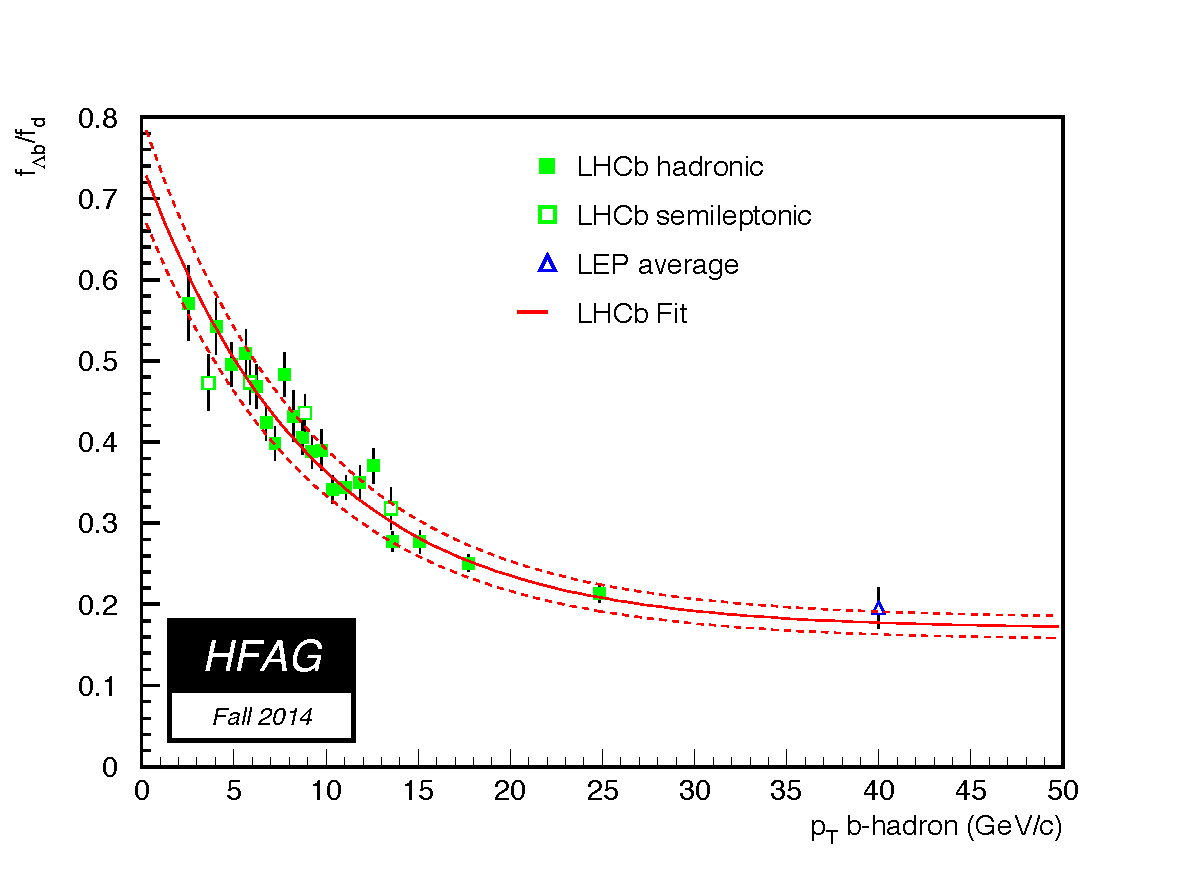
\includegraphics[width=\textwidth]{figures/life_mix/rlb_comb}
  \caption{Ratio of production fractions $\fLb/\fBd$ as 
   a function of $p_{\rm T}$ of the \b hadron from
   LHCb data for \b hadrons decaying semileptonically~\cite{Aaij:2011jp}
   and fully reconstructed in hadronic decays~\cite{Aaij:2014jyk}. 
%   A scale uncertainty due to the common systematic uncertainty 
%   from the $\Lambda_c^+ \rightarrow pK^-\pi^+$ branching fraction
%   is omitted.
   The curve represents a fit to the LHCb hadronic data~\cite{Aaij:2014jyk}.
   The computed LEP ratio is included at an approximate $p_{\rm T}$ 
   in $Z$ decays, but does not participate in any fit.}
  \labf{rlb_comb}
 \end{center}
\end{figure}

Both CDF and LHCb have investigated the $p_{\rm T}$ dependence of $\fBs/\fBd$ using fully 
reconstructed $\Bs$ and $\Bd$ decays.  The CDF analysis reconstructed decays that include 
a $J/\psi$ in the final state~\cite{CDFnote10795:2012} and reports no significant $p_{\rm T}$ dependence 
on the ratio.  However, their result is dominated by an $18$\% scale uncertainty
from preliminary measurements of the branching ratios of the $\BR{\Bs\to J/\psi \phi}$ and 
$\BR{\Bd\to J\psi K^{*}(892)}$.
LHCb reported $3\sigma$ evidence that the ratio $\fBs/\fBd$ decreases with 
$p_{\rm T}$ using fully reconstructed $\Bs$ and $\Bd$ decays and theoretical predictions for branching ratios~\cite{Aaij:2013qqa}. \Figure{rs_comb} shows
the ratio $R_s = \fBs/\fBu$ as a function of $p_{\rm T}$ measured by CDF and LHCb.
Two fits are performed similar to the result for $R_{\Lambda_b}$ above.  The first
fit using a linear parameterization yields
$R_s = (0.2760\pm 0.0068) - (0.00191\pm 0.00059)\times p_{\rm T}$.  
A second fit using a simple exponential yields
$R_s = \exp\left\{(-1.293\pm 0.028) - (0.0077\pm 0.0025)\times p_{\rm T}\right\}$.  
The two fits are nearly indistinguisible over the $p_{\rm T}$ range of the results
but the second gives a physical value for all $p_{\rm T}$.  $R_s$ is also calculated
for LEP and placed at the approximate $p_{\rm T}$ for the $b$ hadron, though the LEP result
doesn't participate in the fit.  The PDG world average for $R_s$ is also included in the
figure for reference.

\begin{figure}
 \begin{center}
  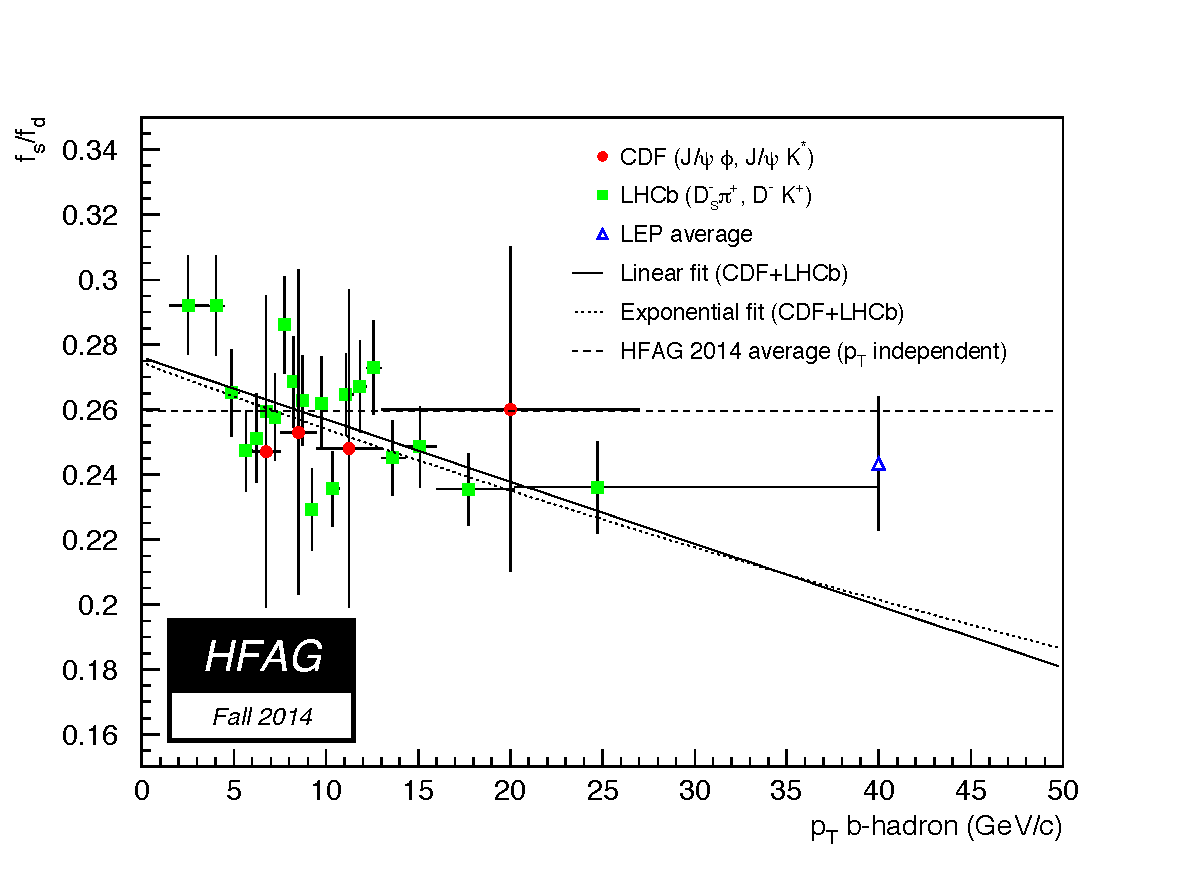
\includegraphics[width=\textwidth]{figures/life_mix/rs_comb}
  \caption{Ratio of production fractions $\fBs/\fBd$ as 
   a function of $p_{\rm T}$ of the reconstructed $b$-hadrons for the 
   CDF~\cite{CDFnote10795:2012} and LHCb~\cite{Aaij:2013qqa} 
   data. Note the suppressed zero for the vertical axis.
   The curves represent fits to the data:
   a linear fit (solid), and an exponential fit described in the text (dotted).
   The $p_{\rm T}$ independent value average of $R_s$ (dashed) is shown for 
   comparison.
   The computed LEP ratio is included at an 
   approximate $p_{\rm T}$ in $Z$ decays, but does not participate in any fit.}
  \labf{rs_comb}
 \end{center}
\end{figure}

In order to combine or compare LHCb results with other experiments,
the $p_{\rm T}$-dependent $\fLb/(\fBu + \fBd)$ is weighted by the $p_{\rm T}$ spectrum\footnote{
  \label{foot:life_mix:Aaij:2011jp}
  In practice the LHCb data are given in 14 bins in $p_{\rm T}$ and $\eta$ with a full covariance matrix~\cite{Aaij:2011jp}. 
  The weighted average is calculated as
  $D^T C^{-1} M/\sigma$, where $\sigma = D^T C^{-1} D$, $M$ is a vector 
  of measurements, $C^{-1}$ is the inverse covariance matrix and $D^T$ is the 
  transpose of the design matrix (vector of 1's)}. 
\Table{LHCBcomp} compares 
the $p_{\rm T}$-weighted LHCb data with comparable averages from CDF. 
The average CDF 
and LHCb data are in good agreement despite the \b hadrons being produced 
in different kinematic regimes.

\begin{table}
 \caption{Comparison of average production fraction ratios from CDF and LHCb.
 The kinematic regime of the charm+lepton system reconstructed in each
 experiment is also shown.}
 \labt{LHCBcomp}
 \begin{center}
  \begin{tabular}{lccc}
   \hline
   Quantity                         & CDF               & LHCb \\
   \hline
   $\fBs/(\fBu + \fBd)$             & \hfagRBSTEVNOCON  & \hfagRBSLHCBNOCON   \\
   $\fLb/(\fBu + \fBd)$             & \hfagRLBTEVNOCON  & \hfagRLBLHCBNOCON   \\
   Average charm+lepton $p_{\rm T}$ & $\sim 13$~GeV/$c$ & $\sim 7$~GeV/$c$ \\
   Pseudo-rapidity range             & $-1 < \eta < 1$   & $2 < \eta < 5$      \\
   \hline
  \end{tabular}
 \end{center}
\end{table}

All these published results have been combined
%\footnote{%
%The latest preliminary results from CDF using $\Bs\to\jpsi\phi$ decays~\cite{CDFnote10795:2012}
%have not been included yet in our averages.
%}
following the procedure and 
assumptions described in \Ref{Abbaneo:2000ej_mod,*Abbaneo:2001bv_mod_cont},
to yield $\fBu=\fBd=\hfagWFBDNOMIX$, 
$\fBs=\hfagWFBSNOMIX$ and $\fbb=\hfagWFBBNOMIX$
under the constraints of \Eq{constraints}.  
%Following the PDG prescription, we have scaled the combined uncertainties 
%on these fractions by \hfagWFSFACTOR to account for slight discrepancies 
%in the input data. 
Repeating the combinations, for LEP and the Tevatron, we obtain 
$\fBu=\fBd=\hfagZFBDNOMIX$,
$\fBs=\hfagZFBSNOMIX$ and $\fbb=\hfagZFBBNOMIX$ when using the LEP data only,
$\fBu=\fBd=\hfagTFBDNOMIX$, $\fBs=\hfagTFBSNOMIX$ 
$\fbb = \hfagTFBBNOMIX$ when using the Tevatron data only.  As noted previously,
the LHCb data are insufficient to determine a complete set of \b-hadron production
fractions. The world averages (LEP, Tevatron and LHCb) for the various fractions 
are presented here for comparison with previous averages.  Significant differences
exist between the LEP and Tevatron fractions, therefore use of the world averages
should be taken with some care.
%When the Tevatron, 
%LHCb and LEP data are separated, we find no need to scale the uncertainties of 
%any combination.  
For these combinations other external inputs are used, 
\eg\ the branching ratios of \B mesons to final states with a \particle{D}, 
\particle{D^*} or \particle{D^{**}} in semileptonic decays, which are needed 
to evaluate the fraction of semileptonic \Bs decays with a \particle{D_s^-} 
in the final state.


Time-integrated mixing analyses performed with lepton pairs 
from \particle{b\bar{b}} 
events produced at high-energy colliders measure the quantity 
\begin{equation}
\chibar = f'_{\particle{d}} \,\chid + f'_{\particle{s}} \,\chis \,,
\labe{chibar}
\end{equation}
where $f'_{\particle{d}}$ and $f'_{\particle{s}}$ are 
the fractions of \Bd and \Bs hadrons 
in a sample of semileptonic \b-hadron decays, and where \chid and \chis 
are the \Bd and \Bs time-integrated mixing probabilities.
Assuming that all \b hadrons have the same semileptonic decay width implies 
$f'_i = f_i R_i$, where $R_i = \tau_i/\tau_{\b}$ is the ratio of the lifetime 
$\tau_i$ of species $i$ to the average \b-hadron lifetime 
$\tau_{\b} = \sum_i f_i \tau_i$.
Hence measurements of the mixing probabilities
\chibar, \chid and \chis can be used to improve our 
knowledge of \fBu, \fBd, \fBs and \fbb.
In practice, the above relations yield another determination of 
\fBs obtained from \fbb and mixing information, 
\begin{equation}
\fBs = \frac{1}{R_{\particle{s}}}
\frac{(1+r)\overline{\chi}-(1-\fbb R_{\rm baryon}) \chid}{(1+r)\chis - \chid} \,,
\labe{fBs-mixing}
\end{equation}
where $r=R_{\particle{u}}/R_{\particle{d}} = \tau(\Bu)/\tau(\Bd)$.

The published measurements of \chibar performed by the LEP
experiments have been combined by the LEP Electroweak Working Group to yield 
$\chibar = \hfagCHIBARLEP$~\cite{LEPEWWG:2005ema_mod}.
This can be compared with the Tevatron average, $\chibar = \hfagCHIBARTEV$,
obtained from \dzero~\cite{Abazov:2006qw} and CDF~\cite{CDFnote10335:2011}
measurements with Run~II data.\footnote{
  \label{foot:life_mix:Acosta:2003ie_mod}
  As explained in \Ref{CDFnote10335:2011}, a previous CDF analysis~\cite{Acosta:2003ie_mod}
  performed with Run~I data overlooked a background component, so the corresponding result is not 
  included in the average.}
%old% The two averages deviate
%old% from each other by $\hfagCHIBARSFACTOR\,\sigma$; 
%old% this could be an indication that the production fractions of \b hadrons 
%old% at the \particle{Z} peak or at the Tevatron are not the same. 
%old% Although this discrepancy 
%old% is not very significant it should be carefully monitored in the future. 
%old% We choose to combine these two results in a simple weighted average,
%old% assuming no correlations, and, following the PDG prescription, we 
%old% multiply the combined uncertainty by \hfagCHIBARSFACTOR to account 
%old% for the discrepancy. Our world average is then $\chibar = \hfagCHIBAR$.
The two averages agree, showing no evidence that the production fractions
of \Bd and \Bs mesons at the \particle{Z} peak or at the Tevatron are different.
We combine these two results in a simple weighted average,
assuming no correlations, and obtain 
$\chibar = \hfagCHIBAR$.

\begin{table}
\caption{Time-integrated mixing probability \chibar (defined in \Eq{chibar}), 
and fractions of the different \b-hadron species in an unbiased sample of 
weakly-decaying \b hadrons, obtained from both direct
and mixing measurements. The correlation coefficients between the fractions are 
also given.
The last column includes measurements performed at LEP, Tevatron and LHCb.}
\labt{fractions}
\begin{center}
\begin{tabular}{@{}l@{~}l@{~}cccc@{}}
\hline
Quantity            &                      & $Z$ decays      & Tevatron       & LHCb~\cite{Aaij:2013qqa} & all    \\
\hline
Mixing probability  & $\overline{\chi}$    & \hfagCHIBARLEP  & \hfagCHIBARTEV &         & \hfagCHIBAR \\
\Bu or \Bd fraction & $\fBu = \fBd$        & \hfagZFBD       & \hfagTFBD      &         & \hfagWFBD   \\
\Bs fraction        & $\fBs$               & \hfagZFBS       & \hfagTFBS      &         & \hfagWFBS   \\
\b-baryon fraction  & $\fbb$               & \hfagZFBB       & \hfagTFBB      &         & \hfagWFBB   \\
$\Bs/\Bd$ ratio     & $\fBs/\fBd$          & \hfagZFBSBD     & \hfagTFBSBD    & $0.256 \pm 0.020$ & \hfagWFBSBD \\
\multicolumn{2}{@{}l}{$\rho(\fBs,\fBu) = \rho(\fBs,\fBd)$} & \hfagZRHOFBDFBS & \hfagTRHOFBDFBS &         & \hfagWRHOFBDFBS \\
\multicolumn{2}{@{}l}{$\rho(\fbb,\fBu) = \rho(\fbb,\fBd)$} & \hfagZRHOFBDFBB & \hfagTRHOFBDFBB &         & \hfagWRHOFBDFBB \\
\multicolumn{2}{@{}l}{$\rho(\fbb,\fBs)$}                   & \hfagZRHOFBBFBS & \hfagTRHOFBBFBS &         & \hfagWRHOFBBFBS \\
\hline
\end{tabular}
\end{center}
\end{table}

Introducing the \chibar average in \Eq{fBs-mixing}, together with our world average 
$\chid = \hfagCHIDWU$ (see \Eq{chid} of \Sec{dmd}), the assumption $\chis= 1/2$ 
(justified by \Eq{chis} in \Sec{dms}), the 
best knowledge of the lifetimes (see \Sec{lifetimes}) and the estimate of \fbb given above, 
yields $\fBs = \hfagWFBSMIX$ 
(or $\fBs = \hfagZFBSMIX$ using only LEP data, 
or $\fBs = \hfagTFBSMIX$ using only Tevatron data),
an estimate dominated by the mixing information. 
Taking into account all known correlations (including the one introduced by \fbb), 
this result is then combined with the set of fractions obtained from direct measurements 
(given above), to yield the % following improved estimates, 
improved estimates of \Table{fractions}, 
still under the constraints of \Eq{constraints}.
%%% \footnote{%
%%% The combined value of \fbb is smaller than the  
%%% results from either LEP, the Tevatron and LHCb separately.
%%% This seemingly surprising result  
%%% arises from the smaller uncertainties on the other fractions 
%%% and the application of the unitarity constraint of \Eq{constraints}.}
As can be seen, our knowledge on the mixing parameters 
substantially reduces the uncertainty on \fBs.
% , and this even in the case of the world averages where a rather strong deweighting was introduced in the computation of \chibar.
It should be noted that the results % of \Eqsss{fBd}{fBs}{fbb} 
are correlated, as indicated in \Table{fractions}.

%------------------------------------------------
%\mysubsection{\b-hadron lifetimes}
%------------------------------------------------

% Introduction, b-hadron lifetime, B0 lifetime, B+ lifetime, B+/B0 lifetime ratio
%%%%%%%%%%%%%%%%%%%%%%%%%%%%%%%%%%%%%%%%%%%%%%%%%%
%
% This is file life_mix_tau1.tex containing the
% first part of the chapter on the b-hadron life-
% times: introduction, average b-hadron, B0 and B+
% lifetimes as well as the B+/B0 lifetime ratio
%
%%%%%%%%%%%%%%%%%%%%%%%%%%%%%%%%%%%%%%%%%%%%%%%%%

%------------------------------------------------
\mysubsection{\b-hadron lifetimes}
%------------------------------------------------
\labs{lifetimes}

In the spectator model the decay of \b-flavoured hadrons $H_b$ is
governed entirely by the flavour changing \particle{b\to Wq} transition
($\particle{q}=\particle{c,u}$).  For this very reason, lifetimes of all
\b-flavoured hadrons are the same in the spectator approximation
regardless of the (spectator) quark content of the $H_b$.  In the early
1990's experiments became sophisticated enough to start seeing the
differences of the lifetimes among various $H_b$ species.  The first
theoretical calculations of the spectator quark effects on $H_b$
lifetime emerged only few years earlier.

Currently, most of such calculations are performed in the framework of
the Heavy Quark Expansion, HQE.  In the HQE, under certain assumptions
(most important of which is that of quark-hadron duality), the decay
rate of an $H_b$ to an inclusive final state $f$ is expressed as the sum
of a series of expectation values of operators of increasing dimension,
multiplied by the correspondingly higher powers of $\Lambda_{\rm
QCD}/m_b$:
\begin{equation}
\Gamma_{H_b\to f} = |CKM|^2\sum_n c_n^{(f)}
\Bigl(\frac{\Lambda_{\rm QCD}}{m_b}\Bigr)^n\langle H_b|O_n|H_b\rangle,
\labe{hqe}
\end{equation}
where $|CKM|^2$ is the relevant combination of the CKM matrix elements.
Coefficients $c_n^{(f)}$ of this expansion, known as Operator Product
Expansion~\cite{Shifman:1986mx,*Chay:1990da,*Bigi:1992su,*Bigi:1992su_erratum},
can be calculated perturbatively.  Hence, the HQE
predicts $\Gamma_{H_b\to f}$ in the form of an expansion in both
$\Lambda_{\rm QCD}/m_{\b}$ and $\alpha_s(m_{\b})$.  The precision of
current experiments makes it mandatory to go to the next-to-leading
order in QCD, {\em i.e.}\ to include correction of the order of
$\alpha_s(m_{\b})$ to the $c_n^{(f)}$'s.  All non-perturbative physics
is shifted into the expectation values $\langle H_b|O_n|H_b\rangle$ of
operators $O_n$.  These can be calculated using lattice QCD or QCD sum
rules, or can be related to other observables via the
HQE~\cite{Bigi:1995jr,*Bellini:1996ra}.  One may reasonably expect that powers of
$\Lambda_{\rm QCD}/m_{\b}$ provide enough suppression that only the
first few terms of the sum in \Eq{hqe} matter.

Theoretical predictions are usually made for the ratios of the lifetimes
(with $\tau(\Bd)$ chosen as the common denominator) rather than for the
individual lifetimes, for this allows several uncertainties to cancel.
The precision of the current HQE calculations (see
\Refs{Ciuchini:2001vx,*Beneke:2002rj,*Franco:2002fc,Tarantino:2003qw,*Gabbiani:2003pq,Gabbiani:2004tp} for the latest updates)
is in some instances already surpassed by the measurements,
\eg\ in the case of $\tau(\Bu)/\tau(\Bd)$.  Also, HQE calculations are
not assumption-free.  More accurate predictions are a matter of progress
in the evaluation of the non-perturbative hadronic matrix elements and
verifying the assumptions that the calculations are based upon.
However, the HQE, even in its present shape, draws a number of important
conclusions, which are in agreement with experimental observations:
\begin{itemize}
\item The heavier the mass of the heavy quark the smaller is the
  variation in the lifetimes among different hadrons containing this
  quark, which is to say that as $m_{\b}\to\infty$ we retrieve the
  spectator picture in which the lifetimes of all $H_b$'s are the same.
%OS  This is well illustrated by the fact that lifetimes in the $b$ sector
%OS  are all rather similar, while in the $c$ sector
%OS  ($m_{\particle{c}}<m_{\b}$) lifetimes differ by large factors.
   This is well illustrated by the fact that lifetimes are rather
   similar in the \b sector, while they differ by large factors
   in the \particle{c} sector ($m_{\particle{c}}<m_{\b}$).
\item The non-perturbative corrections arise only at the order of
  $\Lambda_{\rm QCD}^2/m_{\b}^2$, which translates into 
  differences among $H_b$ lifetimes of only a few percent.
\item It is only the difference between meson and baryon lifetimes that
  appears at the $\Lambda_{\rm QCD}^2/m_{\b}^2$ level.  The splitting of the
  meson lifetimes occurs at the $\Lambda_{\rm QCD}^3/m_{\b}^3$ level, yet it is
  enhanced by a phase space factor $16\pi^2$ with respect to the leading
  free \b decay.
\end{itemize}

To ensure that certain sources of systematic uncertainty cancel, 
lifetime analyses are sometimes designed to measure a 
ratio of lifetimes.  However, because of the differences in decay
topologies, abundance (or lack thereof) of decays of a certain kind,
{\em etc.}, measurements of the individual lifetimes are more 
common.  In the following section we review the most common
types of the lifetime measurements.  This discussion is followed by the
presentation of the averaging of the various lifetime measurements, each
with a brief description of its particularities.


%% Experimental measurements too often benefit from a partial systematic
%% uncertainty cancellation if a measurement is that of the ratio of two
%% quantities of the same kind, which are affected similarly by one or
%% more systematic effect(s).  For this reason, rather often the lifetime
%% measurements are being designed to be those of the ratio of the
%% lifetimes.  However, because of the differences in decay topologies,
%% abundance (or lack thereof) of decays of a certain kind, {\em etc.}\
%% measurements of the individual lifetimes are not particularly rare.  In
%% the following section we review the most common types of the lifetime
%% measurements.  This discussion is followed by the presentation of the
%% averaging of the various lifetime measurements, each with a brief
%% description of its particularities.

%% Details of procedures used to combine the different measurements can be
%% found in \Ref{LEPBOSC:1996}. {\sc do we want this? HERE?}


\mysubsubsection{Lifetime measurements, uncertainties and correlations}

In most cases lifetime of an $H_b$ is estimated from a flight distance
and a $\beta\gamma$ factor which is used to convert the geometrical
distance into the proper decay time.  Methods of accessing lifetime
information can roughly be divided in the following five categories:
\begin{enumerate}
\item {\bf\em Inclusive (flavour-blind) measurements}.  These
  measurements are aimed at extracting the lifetime from a mixture of
  \b-hadron decays, without distinguishing the decaying species.  Often
  the knowledge of the mixture composition is limited, which makes these
  measurements experiment-specific.  Also, these
  measurements have to rely on Monte Carlo for estimating the
  $\beta\gamma$ factor, because the decaying hadrons are not fully
  reconstructed.  On the bright side, these usually are the largest
  statistics \b-hadron lifetime measurements that are accessible to a
  given experiment, and can, therefore, serve as an important
  performance benchmark.
\item {\bf\em Measurements in semileptonic decays of a specific
  {\boldmath $H_b$\unboldmath}}.  \particle{W}from \particle{\b\to Wc}
  produces $\ell\nu_l$ pair (\particle{\ell=e,\mu}) in about 21\% of the
  cases.  Electron or muon from such decays is usually a well-detected
  signature, which provides for clean and efficient trigger.
  \particle{c} quark from \particle{b\to Wc} transition and the other
  quark(s) making up the decaying $H_b$ combine into a charm hadron,
  which is reconstructed in one or more exclusive decay channels.
  Knowing what this charmed hadron is allows one to separate, at least
  statistically, different $H_b$ species.  The advantage of these
  measurements is in statistics, which usually is superior to that of the
  exclusively reconstructed $H_b$ decays.  Some of the main
  disadvantages are related to the difficulty of estimating lepton+charm
  sample composition and Monte Carlo reliance for the $\beta\gamma$
  factor estimate.
\item {\bf\em Measurements in exclusively reconstructed hadronic decays}.
  These
  have the advantage of complete reconstruction of decaying $H_b$, which
  allows one to infer the decaying species as well as to perform precise
  measurement of the $\beta\gamma$ factor.  Both lead to generally
  smaller systematic uncertainties than in the above two categories.
  The downsides are smaller branching ratios, larger combinatoric
  backgrounds, especially in $H_b\rightarrow H_c\pi(\pi\pi)$ and
  multi-body $H_c$ decays, or in a hadron collider environment with
  non-trivial underlying event.  $H_b\to \jpsi H_s$ are relatively
  clean and easy to trigger on $\jpsi\to \ell^+\ell^-$, but their
  branching fraction is only about 1\%.
\item {\bf\em Measurements at asymmetric B factories}. 

In the $\Ups\rightarrow B \bar{B}$ decay, the \B mesons (\Bu or \Bd) are
essentially at rest in the \Ups frame.  This makes direct lifetime
measurements impossible in experiments at symmetric colliders producing 
\Ups at rest. 
%Romulus% However, most time-integrated measurements that related to
%Romulus% directly measure the overall mixing probability, \chid, have been measured
%Romulus% by the CLEO and ARGUS. It is almost impossible to measure the \B mesons lifetime measurement
%Romulus% with time-integrated technique. The best approach for measuring the \B mesons lifetime 
%Romulus% is using the time dependent measurement at asymmetric \B factories such as \babar and
%Romulus% Belle. 
At asymmetric \B factories the \Ups meson is boosted
resulting in \B and \particle{\bar{B}} moving nearly parallel to each 
other with the same boost. The lifetime is inferred from the distance $\Delta z$        
separating the \B and \particle{\bar{B}} decay vertices along the beam axis 
%Romulus% (see \Fig{Ups_geometry})
and from the \Ups boost known from the beam energies. This boost is equal to 
$\beta \gamma \approx 0.55$ (0.43) in the \babar (\belle) experiment,
resulting in an average \B decay length of approximately 250~(190)~$\mu$m. 
%Romulus% \begin{figure}
%Romulus% \begin{center}
%Romulus% \epsfig{figure=figures/life_mix/Ups_geometry.eps,width=0.6\textwidth}
%Romulus% \caption{\Ups decay in the laboratory frame where one \B meson is fully 
%Romulus% reconstructed}
%Romulus% \labf{Ups_geometry}
%Romulus% \end{center}
%Romulus% \end{figure}

%Romulus% At asymmetric \B factories, the \Ups decays only to a pair of \B mesons since the mass of 
%Romulus% the \Ups is about 22 $MeV$ above \B mesons pair with no additional pions or any other
%Romulus% type of $b$ hadrons produced.  Both \B mesons produced from the \Ups decays move away 
%Romulus% from the production vertex nearly parallel to each other by a few hundred microns before
%Romulus% decaying due to a boost in the beam direction. For \babar the boost is $<\beta \gamma> \approx 0.55$ and
%Romulus% for Belle is $<\beta \gamma> \approx 0.43$. The lifetime is inferred from the distance $\Delta z$
%Romulus% separating \B and \particle{\bar{B}} decay vertexes and \Ups boost
%Romulus% known from colliding beam energies.  

%OS In order to maximize the
%OS precision of the measurement, one \B meson is reconstructed in the
%OS \particle{D^{(*)}\ell\nu_{\ell}} decay.  The other \B is typically not
%OS fully reconstructed, only position of its decay vertex is determined.

%Romulus% The geometry of an \Ups decay to a pair of \B mesons in which one \B meson is fully 
%Romulus% reconstructed is shown in \Fig{Ups_geometry}. 
%Romulus% At \babar the average decay length is of the order of 
%Romulus% 250~$\mu$m and the uncertainty for a vertex point are about $\approx$ 50~$\mu$m for a fully
%Romulus% reconstructed \B meson and $\approx 100~\mu$m for a partially reconstructed \B meson.
In order to determine the charge of the \B mesons in each event, one of the them is
fully reconstructed in a semileptonic or hadronic decay mode.
The other \B is typically not fully reconstructed, only the position
of its decay vertex is determined from the remaining tracks in the event.
These measurements benefit from large statistics, but suffer from poor proper time 
resolution, comparable to the \B lifetime itself. This resolution is dominated by the 
uncertainty on the decay vertices, which is typically 50~(100)~$\mu$m for a
fully (partially) reconstructed \B meson. 
%Romulus% $\Delta z$ resolution.
%Romulus% At asymmetric \B factories, the decay time different resolution is dominated by the uncertainty 
%Romulus% of the vertex location of both \B mesons. The decay distance and the momenta of a \B meson 
%Romulus% determine its lifetime. In order to determine the charge of the \B mesons in each event,
%Romulus% one of the them is fully reconstructed in semileptonic or fully hadronic decay modes.
%Romulus% The other \B is typically not fully reconstructed, only the position
%Romulus% of its decay vertex is determined from the remaining tracks in the event.
%Romulus% These measurements benefit from very large statistics, but suffer from
%Romulus% poor $\Delta z$ resolution (the distance between the two \B mesons decay
%Romulus% vertexes projected on the beam axis.
%Romulus% Alternatively one could apply a completely 
%Romulus% reconstructed events where both \B are fully reconstructed for getting the best
%Romulus% precision on the lifetime measurement, however, a price has to be paid due to 
%Romulus% a low statistics. 
With very large future statistics,
the resolution and purity could be improved (and hence the systematics reduced)
by fully reconstructing both \B mesons in the event. 
 
\item {\bf\em Direct measurement of lifetime ratios}.  This method has
  so far been only applied in the measurement of $\tau(\Bu)/\tau(\Bd)$.
  The ratio of the lifetimes is extracted from the dependence of the
  observed relative number of \Bu and \Bd candidates (both reconstructed
  in semileptonic decays) on the proper decay time.
\end{enumerate}

In some of the latest analyses, measurements of two (\eg\ $\tau(\Bu)$ and
$\tau(\Bu)/\tau(\Bd)$) or three (\eg\ $\tau(\Bu)$,
$\tau(\Bu)/\tau(\Bd)$, and \dmd) quantities are combined.  This
introduces correlations among measurements.  Another source of
correlations among the measurements are the systematic effects, which
could be common to an experiment or to an analysis technique across the
experiments.  When calculating the averages, such correlations are taken
into account per general procedure, described in
\Ref{LEPBOSC:1996}.


%% ====================================================================
\mysubsubsection{Inclusive \b-hadron lifetimes}
%% ====================================================================

The inclusive \b hadron lifetime is defined as $\tau_{\b} = \sum_i f_i
\tau_i$ where $\tau_i$ are the individual species lifetimes and $f_i$ are
the fractions of the various species present in an unbiased sample of
weakly-decaying \b hadrons produced at a high-energy
collider.\footnote{In principle such a quantity could be slightly
different in \particle{Z} decays and at the Tevatron, in case the
fractions of \b-hadron species are not exactly the same; see the
discussion in \Sec{fractions_high_energy}.}  This quantity is certainly
less fundamental than the lifetimes of the individual species, the
latter being much more useful in comparisons of the measurements with
the theoretical predictions.  Nonetheless, we perform the averaging of
the inclusive lifetime measurements for completeness as well as for the
reason that they might be of interest as ``technical numbers.''

\begin{table}[tp]
\caption{Measurements of average \b-hadron lifetimes.}
\labt{lifeincl}
\begin{center}
\begin{tabular}{lcccl} \hline
Experiment &Method           &Data set & $\tau_{\b}$ (ps)       &Ref.\\
\hline
ALEPH  &Dipole               &91     &$1.511\pm 0.022\pm 0.078$ &\cite{Buskulic:1993gj}\\
DELPHI &All track i.p.\ (2D) &91--92 &$1.542\pm 0.021\pm 0.045$ &\cite{Abreu:1994dr}$^a$\\
DELPHI &Sec.\ vtx            &91--93 &$1.582\pm 0.011\pm 0.027$ &\cite{Abreu:1996hv}$^a$\\
DELPHI &Sec.\ vtx            &94--95 &$1.570\pm 0.005\pm 0.008$ &\cite{Abdallah:2003sb}\\
L3     &Sec.\ vtx + i.p.     &91--94 &$1.556\pm 0.010\pm 0.017$ &\cite{Acciarri:1997tt}$^b$\\
OPAL   &Sec.\ vtx            &91--94 &$1.611\pm 0.010\pm 0.027$ &\cite{Ackerstaff:1996as}\\
SLD    &Sec.\ vtx            &93     &$1.564\pm 0.030\pm 0.036$ &\cite{Abe:1995rm}\\ 
\hline
\multicolumn{2}{l}{Average set 1 (\b vertex)} && \hfagTAUBVTXnounit &\\
\hline\hline
ALEPH  &Lepton i.p.\ (3D)    &91--93 &$1.533\pm 0.013\pm 0.022$ &\cite{Buskulic:1995rw}\\
L3     &Lepton i.p.\ (2D)    &91--94 &$1.544\pm 0.016\pm 0.021$ &\cite{Acciarri:1997tt}$^b$\\
OPAL   &Lepton i.p.\ (2D)    &90--91 &$1.523\pm 0.034\pm 0.038$ &\cite{Acton:1993xk}\\ 
\hline
\multicolumn{2}{l}{Average set 2 ($\b\to\ell$)} && \hfagTAUBLEPnounit &\\
\hline\hline
CDF1   &\particle{\jpsi} vtx&92--95 &$1.533\pm 0.015^{+0.035}_{-0.031}$ &\cite{Abe:1997bd} \\ 
%% CDF2       & \particle{\jpsi} vtx
%%                                &  02--03 & $1.526 \pm 0.034 \pm 0.035$ & \cite{CDFnote9203:2008,*CDFnote9203:2008_cont} \\  WARNING: the meaning of CDFnote9203:2008 has changed !!!
ATLAS &\particle{\jpsi} vtx& 2010 & $1.489\pm 0.016 \pm 0.043$ & \cite{ATLAS-CONF-2011-145}$^p$ \\
\hline
\multicolumn{2}{l}{Average set 3 (\particle{\b\to \jpsi})} && \hfagTAUBJPnounit & \\ 
%\hline\hline
%\multicolumn{2}{l}{Average of all above} && \hfagTAUBnounit & \\
\hline
\multicolumn{5}{l}{$^a$ \footnotesize The combined DELPHI result quoted in
\cite{Abreu:1996hv} is 1.575 $\pm$ 0.010 $\pm$ 0.026 ps.} \\[-0.5ex]
\multicolumn{5}{l}{$^b$ \footnotesize The combined L3 result quoted in \cite{Acciarri:1997tt} 
is 1.549 $\pm$ 0.009 $\pm$ 0.015 ps.} \\[-0.5ex]
\multicolumn{5}{l}{$^p$ \footnotesize Preliminary.}
\end{tabular}
\end{center}
\end{table}

In practice, an unbiased measurement of the inclusive lifetime is
difficult to achieve, because it would imply an efficiency which is
guaranteed to be the same across species.  So most of the measurements
are biased.  In an attempt to group analyses which are expected to
select the same mixture of \b hadrons, the available results (given in
\Table{lifeincl}) are divided into the following three sets:
\begin{enumerate}
\item measurements at LEP and SLD that accept any \b-hadron decay, based 
      on topological reconstruction (secondary vertex or track impact
      parameters);
\item measurements at LEP based on the identification
      of a lepton from a \b decay; and
\item measurements at the Tevatron based on inclusive 
      \particle{H_b\to \jpsi X} reconstruction, where the
      \particle{\jpsi} is fully reconstructed.
\end{enumerate}

The measurements of the first set are generally considered as estimates
of $\tau_{\b}$, although the efficiency to reconstruct a secondary
vertex most probably depends, in an analysis-specific way, on the number
of tracks coming from the vertex, thereby depending on the type of the
$H_b$.  Even though these efficiency variations can in principle be
accounted for using Monte Carlo simulations (which inevitably contain
assumptions on branching fractions), the $H_b$ mixture in that case can
remain somewhat ill-defined and could be slightly different among
analyses in this set.

On the contrary, the mixtures corresponding to the other two sets of
measurements are better defined in the limit where the reconstruction
and selection efficiency of a lepton or a \particle{\jpsi} from an
$H_b$ does not depend on the decaying hadron type.  These mixtures are
given by the production fractions and the inclusive branching fractions
for each $H_b$ species to give a lepton or a \particle{\jpsi}.  In
particular, under the assumption that all \b hadrons have the same
semileptonic decay width, the analyses of the second set should measure
$\tau(\b\to\ell) = (\sum_i f_i \tau_i^3) /(\sum_i f_i \tau_i^2)$ which is
necessarily larger than $\tau_{\b}$ if lifetime differences exist.
Given the present knowledge on $\tau_i$ and $f_i$,
$\tau(\b\to\ell)-\tau_{\b}$ is expected to be of the order of 0.003\ps.
On the other hand, the third set measuring $\tau(\b\to\particle{\jpsi})$
is expected to give an average smaller than $\tau_{\b}$ because 
of the \Bc meson which has a significantly
larger probability to decay to a \particle{\jpsi}
than other \b-hadron species. 

Measurements by SLC and LEP experiments are subject to a number of
common systematic uncertainties, such as those due to (lack of knowledge
of) \b and \particle{c} fragmentation, \b and \particle{c} decay models,
\BR{B\to\ell}, \BR{B\to c\to\ell}, \BR{c\to\ell}, $\tau_{\particle{c}}$,
and $H_b$ decay multiplicity.  In the averaging, these systematic
uncertainties are assumed to be 100\% correlated.  The averages for the
sets defined above (also given in \Table{lifeincl}) are
\begin{eqnarray}
\tau(\b~\mbox{vertex}) &=& \hfagTAUBVTX \,, \labe{TAUBVTX} \\
\tau(\b\to\ell) &=& \hfagTAUBLEP  \,, \\
\tau(\b\to\particle{\jpsi}) &=& \hfagTAUBJP\,.
\end{eqnarray}
% whereas an average of all measurements, ignoring mixture differences, 
% yields \hfagTAUB.


%% ====================================================================
\mysubsubsection{\Bd and \Bu lifetimes and their ratio}
%% ====================================================================
\labs{taubd}
\labs{taubu}
\labs{lifetime_ratio}

\begin{table}[tp]
\caption{Measurements of the \Bd lifetime.}
\labt{lifebd}
\begin{center}
\begin{tabular}{lcccl} \hline
Experiment &Method                    &Data set &$\tau(\Bd)$ (ps)                  &Ref.\\
\hline
ALEPH  &\particle{D^{(*)} \ell}       &91--95 &$1.518\pm 0.053\pm 0.034$          &\cite{Barate:2000bs}\\
ALEPH  &Exclusive                     &91--94 &$1.25^{+0.15}_{-0.13}\pm 0.05$     &\cite{Buskulic:1996hy}\\
ALEPH  &Partial rec.\ $\pi^+\pi^-$    &91--94 &$1.49^{+0.17+0.08}_{-0.15-0.06}$   &\cite{Buskulic:1996hy}\\
DELPHI &\particle{D^{(*)} \ell}       &91--93 &$1.61^{+0.14}_{-0.13}\pm 0.08$     &\cite{Abreu:1995mc}\\
DELPHI &Charge sec.\ vtx              &91--93 &$1.63 \pm 0.14 \pm 0.13$           &\cite{Adam:1995mb}\\
DELPHI &Inclusive \particle{D^* \ell} &91--93 &$1.532\pm 0.041\pm 0.040$          &\cite{Abreu:1996gb}\\
DELPHI &Charge sec.\ vtx              &94--95 &$1.531 \pm 0.021\pm0.031$          &\cite{Abdallah:2003sb}\\
L3     &Charge sec.\ vtx              &94--95 &$1.52 \pm 0.06 \pm 0.04$           &\cite{Acciarri:1998uv}\\
OPAL   &\particle{D^{(*)} \ell}       &91--93 &$1.53 \pm 0.12 \pm 0.08$           &\cite{Akers:1995pa}\\
OPAL   &Charge sec.\ vtx              &93--95 &$1.523\pm 0.057\pm 0.053$          &\cite{Abbiendi:1998av}\\
OPAL   &Inclusive \particle{D^* \ell} &91--00 &$1.541\pm 0.028\pm 0.023$          &\cite{Abbiendi:2000ec}\\
SLD    &Charge sec.\ vtx $\ell$       &93--95 &$1.56^{+0.14}_{-0.13} \pm 0.10$    &\cite{Abe:1997ys}$^a$\\
SLD    &Charge sec.\ vtx              &93--95 &$1.66 \pm 0.08 \pm 0.08$           &\cite{Abe:1997ys}$^a$\\
CDF1   &\particle{D^{(*)} \ell}       &92--95 &$1.474\pm 0.039^{+0.052}_{-0.051}$ &\cite{Abe:1998wt}\\
CDF1  &Excl.\ \particle{\jpsi K^{*0}}&92--95 &$1.497\pm 0.073\pm 0.032$          &\cite{Acosta:2002nd}\\
% CDF2  &Excl.\ \particle{\jpsi K^{*0}}&02--04 &$1.541\pm 0.050\pm0.020$           &\cite{Aaltonen:2007gf}\\ %%% Published result superseded by preliminary result of \cite{Aaltonen:2010pj,*Abulencia:2006dr_mod_cont}
%%% CDF2   &Incl.\ \particle{D^{(*)} \ell}&02--04 &$1.473\pm 0.036\pm0.054$           &\cite{CDFnote7514:2005}$^p$\\
%%% CDF2   &Excl.\ \particle{D^-(3)\pi}   &02--04 &$1.511\pm 0.023\pm0.013$           &\cite{CDFnote7386:2005}$^p$\\
CDF2   &Excl.\ \particle {\jpsi K_S}, \particle{\jpsi K^{*0}} &02--09 &$1.507\pm 0.010\pm0.008$           &\cite{Aaltonen:2010pj,*Abulencia:2006dr_mod_cont} \\
%%%%%\dzero &Excl. \particle{\jpsi K^{*0}}&02--04 &$1.473^{+0.052}_{-0.050}\pm0.023$  &\cite{Abazov:2004ce}\\ % superseded by Abazov:2008jz,*Abazov:2005sa_mod_cont
%%%%%\dzero &Excl.\ \particle{\jpsi K^{*0}}&02--05 &$1.530\pm0.043\pm0.023$ &\cite{Abazov:2008jz,*Abazov:2005sa_mod_cont,Abazov:2004ce}\\ % replaces 1.473+0.052-0.050 +-0.023 of \cite{Abazov:2004ce}  % superseded by Abazov:2008jz,*Abazov:2005sa_mod_cont
\dzero &Excl.\ \particle{\jpsi K^{*0}}&03--07 &$1.414\pm0.018\pm0.034$ &\cite{Abazov:2008jz,*Abazov:2005sa_mod_cont}\\ % replaces 1.530+-0.043+-0.023 of above line
\dzero &Excl.\ \particle {\jpsi K_S} &02--11 &$1.508 \pm0.025 \pm0.043$  &\cite{Abazov:2012iy,*Abazov:2007sf_mod_cont,*Abazov:2004bn_mod_cont} \\
\dzero &Inclusive \particle {D^-\mu^+} &02--11 &$1.534 \pm0.019 \pm0.021$  & \cite{Abazov:2014rua,*Abazov:2006cb_cont} \\ % RUN II; 10.4 fb-1
\babar &Exclusive                     &99--00 &$1.546\pm 0.032\pm 0.022$          &\cite{Aubert:2001uw}\\
\babar &Inclusive \particle{D^* \ell} &99--01 &$1.529\pm 0.012\pm 0.029$          &\cite{Aubert:2002gi,*Aubert:2002gi_erratum}\\
\babar &Exclusive \particle{D^* \ell} &99--02 &$1.523^{+0.024}_{-0.023}\pm 0.022$ &\cite{Aubert:2002sh}\\
\babar &Incl.\ \particle{D^*\pi}, \particle{D^*\rho} 
                                      &99--01 &$1.533\pm 0.034 \pm 0.038$         &\cite{Aubert:2002ms}\\
\babar &Inclusive \particle{D^* \ell}
&99--04 &$1.504\pm0.013^{+0.018}_{-0.013}$  &\cite{Aubert:2005kf} \\ 
%% 99 in the above line needs to be verified
%% 04 also. 81/fb, i.e. by summer02 (to be confirmed by David) though reported in summer04
%% lastly, this may actually supersede or have large correlation to \cite{Aubert:2002gi,*Aubert:2002gi_erratum}
%%\belle & Exclusive                     & 00--01 & $1.554\pm 0.030 \pm 0.019$      & \cite{BELLE1}\\
\belle & Exclusive                     & 00--03 & $1.534\pm 0.008\pm0.010$        & \cite{Abe:2004mz}\\
%% in the above Belle not use 99 data, for 140/fb by sum'03
ATLAS & Excl.\ \particle{\jpsi K^{*0}} & 2010 & $1.51 \pm0.04 \pm0.04$ & \cite{ATLAS-CONF-2011-092}$^p$ \\
%%% LHCb  & Excl.\ \particle{\jpsi K^{*0}} & 2010 & $1.512 \pm0.032 \pm 0.042$ & \cite{LHCb-CONF-2011-001}$^p$ \\
LHCb  & Excl.\ \particle{\jpsi K^{*0}} & 2011 & $1.524 \pm0.006 \pm 0.004$ & \cite{Aaij:2014owa} \\
%%% LHCb  & Excl.\ \particle {\jpsi K_S}   & 2010 & $1.558 \pm0.056 \pm 0.022$ & \cite{LHCb-CONF-2011-001}$^p$ \\
LHCb  & Excl.\ \particle {\jpsi K_S}   & 2011 & $1.499 \pm0.013 \pm 0.005$ & \cite{Aaij:2014owa} \\
LHCb    & \particle{K^+\pi^-}   & 2011 & $1.524 \pm 0.011 \pm 0.004$ & \cite{Aaij:2014fia,*Aaij:2012ns_cont} \\
\hline
Average&                               &        & \hfagTAUBDnounit & \\
\hline\hline           
\multicolumn{5}{l}{$^a$ \footnotesize The combined SLD result 
quoted in \cite{Abe:1997ys} is 1.64 $\pm$ 0.08 $\pm$ 0.08 ps.}\\[-0.5ex]
\multicolumn{5}{l}{$^p$ {\footnotesize Preliminary.}}
\end{tabular}
\end{center}
\end{table}

After a number of years of dominating these averages the LEP experiments
yielded the scene to the asymmetric \B~factories and
the Tevatron experiments. The \B~factories have been very successful in
utilizing their potential -- in only a few years of running, \babar and,
to a greater extent, \belle, have struck a balance between the
statistical and the systematic uncertainties, with both being close to
(or even better than) the impressive 1\%.  In the meanwhile, CDF and
\dzero have emerged as significant contributors to the field as the
Tevatron Run~II data flowed in, with CDF eventually providing the most precise results. 
% Both appear to enjoy relatively small
% systematic effects, and while current statistical uncertainties of their
% measurements are factors of 2 to 4 larger than those of their \B-factory
% counterparts, both Tevatron experiments stand to increase their samples
% by almost an order of magnitude.

\begin{table}[tbp]
\caption{Measurements of the \Bu lifetime.}
\labt{lifebu}
\begin{center}
\begin{tabular}{lcccl} \hline
Experiment &Method                 &Data set &$\tau(\Bu)$ (ps)                 &Ref.\\
\hline
ALEPH  &\particle{D^{(*)} \ell}    &91--95 &$1.648\pm 0.049\pm 0.035$          &\cite{Barate:2000bs}\\
ALEPH  &Exclusive                  &91--94 &$1.58^{+0.21+0.04}_{-0.18-0.03}$   &\cite{Buskulic:1996hy}\\
DELPHI &\particle{D^{(*)} \ell}    &91--93 &$1.61\pm 0.16\pm 0.12$             &\cite{Abreu:1995mc}$^a$\\
DELPHI &Charge sec.\ vtx           &91--93 &$1.72\pm 0.08\pm 0.06$             &\cite{Adam:1995mb}$^a$\\
DELPHI &Charge sec.\ vtx           &94--95 &$1.624\pm 0.014\pm 0.018$          &\cite{Abdallah:2003sb}\\
L3     &Charge sec.\ vtx           &94--95 &$1.66\pm  0.06\pm 0.03$            &\cite{Acciarri:1998uv}\\
OPAL   &\particle{D^{(*)} \ell}    &91--93 &$1.52 \pm 0.14\pm 0.09$            &\cite{Akers:1995pa}\\
OPAL   &Charge sec.\ vtx           &93--95 &$1.643\pm 0.037\pm 0.025$          &\cite{Abbiendi:1998av}\\
SLD    &Charge sec.\ vtx $\ell$    &93--95 &$1.61^{+0.13}_{-0.12}\pm 0.07$     &\cite{Abe:1997ys}$^b$\\
SLD    &Charge sec.\ vtx           &93--95 &$1.67\pm 0.07\pm 0.06$             &\cite{Abe:1997ys}$^b$\\
CDF1   &\particle{D^{(*)} \ell}    &92--95 &$1.637\pm 0.058^{+0.045}_{-0.043}$ &\cite{Abe:1998wt}\\
CDF1   &Excl.\ \particle{\jpsi K} &92--95 &$1.636\pm 0.058\pm 0.025$          &\cite{Acosta:2002nd}\\
CDF2   &Excl.\ \particle{\jpsi K} &02--09 &$1.639\pm 0.009\pm 0.009$          &\cite{Aaltonen:2010pj,*Abulencia:2006dr_mod_cont}\\ 
%%% CDF2   &Incl.\ \particle{D^0 \ell} &02--04 &$1.653\pm 0.029^{+0.033}_{-0.031}$ &\cite{CDFnote7514:2005}$^p$\\
CDF2   &Excl.\ \particle{D^0 \pi}  &02--06 &$1.663\pm 0.023\pm0.015$           &\cite{Aaltonen:2010ta}\\
\babar &Exclusive                  &99--00 &$1.673\pm 0.032\pm 0.023$          &\cite{Aubert:2001uw}\\
\belle &Exclusive                  &00--03 &$1.635\pm 0.011\pm 0.011$          &\cite{Abe:2004mz}\\
%%% LHCb  & Excl.\ \particle{\jpsi K} & 2010 & $1.689 \pm0.022 \pm 0.047$ & \cite{LHCb-CONF-2011-001}$^p$ \\
LHCb  & Excl.\ \particle{\jpsi K} & 2011 & $1.637 \pm0.004 \pm 0.003$ & \cite{Aaij:2014owa} \\
\hline
Average&                           &       &\hfagTAUBUnounit &\\
\hline\hline
\multicolumn{5}{l}{$^a$ \footnotesize The combined DELPHI result quoted 
in~\cite{Adam:1995mb} is $1.70 \pm 0.09$ ps.} \\[-0.5ex]
\multicolumn{5}{l}{$^b$ \footnotesize The combined SLD result 
quoted in~\cite{Abe:1997ys} is $1.66 \pm 0.06 \pm 0.05$ ps.}\\[-0.5ex]
% \multicolumn{5}{l}{$^p$ {\footnotesize Preliminary.}}
\end{tabular}
\end{center}
\end{table}


At present time we are in an interesting position of having three sets
of measurements (from LEP/SLC, \B factories and the Tevatron) that
originate from different environments, obtained using substantially
different techniques and are precise enough for incisive comparison.

% While individual lifetimes are often of interest to experiments, \eg\ in
% extraction of CKM matrix elements, the ratios of the lifetimes are more
% interesting from the theoretical perspective as they are predicted more
% precisely.


\begin{table}[tb]
\caption{Measurements of the ratio $\tau(\Bu)/\tau(\Bd)$.}
\labt{liferatioBuBd}
\begin{center}
\begin{tabular}{lcccl} 
\hline
Experiment &Method                 &Data set &Ratio $\tau(\Bu)/\tau(\Bd)$      &Ref.\\
\hline
ALEPH  &\particle{D^{(*)} \ell}    &91--95 &$1.085\pm 0.059\pm 0.018$          &\cite{Barate:2000bs}\\
ALEPH  &Exclusive                  &91--94 &$1.27^{+0.23+0.03}_{-0.19-0.02}$   &\cite{Buskulic:1996hy}\\
DELPHI &\particle{D^{(*)} \ell}    &91--93 &$1.00^{+0.17}_{-0.15}\pm 0.10$     &\cite{Abreu:1995mc}\\
DELPHI &Charge sec.\ vtx           &91--93 &$1.06^{+0.13}_{-0.11}\pm 0.10$     &\cite{Adam:1995mb}\\
DELPHI &Charge sec.\ vtx           &94--95 &$1.060\pm 0.021 \pm 0.024$         &\cite{Abdallah:2003sb}\\
L3     &Charge sec.\ vtx           &94--95 &$1.09\pm 0.07  \pm 0.03$           &\cite{Acciarri:1998uv}\\
OPAL   &\particle{D^{(*)} \ell}    &91--93 &$0.99\pm 0.14^{+0.05}_{-0.04}$     &\cite{Akers:1995pa}\\
OPAL   &Charge sec.\ vtx           &93--95 &$1.079\pm 0.064 \pm 0.041$         &\cite{Abbiendi:1998av}\\
SLD    &Charge sec.\ vtx $\ell$    &93--95 &$1.03^{+0.16}_{-0.14} \pm 0.09$    &\cite{Abe:1997ys}$^a$\\
SLD    &Charge sec.\ vtx           &93--95 &$1.01^{+0.09}_{-0.08} \pm0.05$     &\cite{Abe:1997ys}$^a$\\
CDF1   &\particle{D^{(*)} \ell}    &92--95 &$1.110\pm 0.056^{+0.033}_{-0.030}$ &\cite{Abe:1998wt}\\
CDF1   &Excl.\ \particle{\jpsi K} &92--95 &$1.093\pm 0.066 \pm 0.028$         &\cite{Acosta:2002nd}\\
CDF2   &Excl.\ \particle{\jpsi K^{(*)}} &02--09 &$1.088\pm 0.009 \pm 0.004$   &\cite{Aaltonen:2010pj,*Abulencia:2006dr_mod_cont}\\ 
%%% CDF2   &Incl.\ \particle{D \ell}   &02--04 &$1.123\pm0.040^{+0.041}_{-0.039}$  &\cite{CDFnote7514:2005}$^p$\\
%%% CDF2   &Excl.\ \particle{D \pi}    &02--04 &$1.10\pm 0.02\pm 0.01$             &\cite{CDFnote7386:2005}$^p$\\
\dzero &\particle{D^{*+} \mu} \particle{D^0 \mu} ratio
	                           &02--04 &$1.080\pm 0.016\pm 0.014$          &\cite{Abazov:2004sa}\\
\babar &Exclusive                  &99--00 &$1.082\pm 0.026\pm 0.012$          &\cite{Aubert:2001uw}\\
\belle &Exclusive                  &00--03 &$1.066\pm 0.008\pm 0.008$          &\cite{Abe:2004mz}\\
LHCb  & Excl.\ \particle{\jpsi K^{(*)}} & 2011 & $1.074 \pm0.005 \pm 0.003$ & \cite{Aaij:2014owa} \\
\hline
Average&                           &       & \hfagRTAUBU & \\   
\hline\hline
\multicolumn{5}{l}{$^a$ \footnotesize The combined SLD result quoted
	   in~\cite{Abe:1997ys} is $1.01 \pm 0.07 \pm 0.06$.}
%%% \\[-0.5ex] \multicolumn{5}{l}{$^p$ {\footnotesize Preliminary.}}
\end{tabular}
\end{center}
\end{table}


The averaging of $\tau(\Bu)$, $\tau(\Bd)$ and $\tau(\Bu)/\tau(\Bd)$
measurements is summarized\footnote{
We do not include the old unpublished measurements of Refs.~\cite{CDFnote7514:2005,CDFnote7386:2005}.}
in \Tablesss{lifebd}{lifebu}{liferatioBuBd}.
For $\tau(\Bu)/\tau(\Bd)$ we averaged only the measurements of this
quantity provided by experiments rather than using all available
knowledge, which would have included, for example, $\tau(\Bu)$ and
$\tau(\Bd)$ measurements which did not contribute to any of the ratio
measurements.

The following sources of correlated (within experiment/machine)
systematic uncertainties have been considered:
% (central values and errors scaled accordingly):
\begin{itemize}
\item for SLC/LEP measurements -- \particle{D^{**}} branching ratio uncertainties~\cite{Abbaneo:2000ej_mod,*Abbaneo:2001bv_mod_cont},
momentum estimation of \b mesons from \particle{Z^0} decays
(\b-quark fragmentation parameter $\langle X_E \rangle = 0.702 \pm 0.008$~\cite{Abbaneo:2000ej_mod,*Abbaneo:2001bv_mod_cont}),
\Bs and \b baryon lifetimes (see \Secss{taubs}{taulb}),
and \b-hadron fractions at high energy (see \Table{fractions}); 
\item for \babar measurements -- alignment, $z$ scale, PEP-II boost,
sample composition (where applicable);
\item for \dzero and CDF Run~II measurements -- alignment (separately
within each experiment).
\end{itemize}
The resultant averages are:
\begin{eqnarray}
\tau(\Bd) & = & \hfagTAUBD \,, \\
\tau(\Bu) & = & \hfagTAUBU \,, \\
\tau(\Bu)/\tau(\Bd) & = & \hfagRTAUBU \,.
\end{eqnarray}
  % from Konstantin
% Bs lifetime, Bc lifetime, Lambda_b and b-baryon lifetimes, theoretical predictions
%%%%%%%%%%%%%%%%%%%%%%%%%%%%%%%%%%%%%%%%%%%%%%%%
%
% This is file life_mix_tau2.tex containing
% the second part of the chapter on the b-hadron lifetimes: 
% Bs, Bc, lambda_b and b-baryon lifetimes
% as well as theroretical predictions for all b-hadron lifetimes.
%
%%%%%%%%%%%%%%%%%%%%%%%%%%%%%%%%%%%%%%%%%%%%%%%
%

\mysubsubsection{\Bs lifetimes}
\labs{taubs}

Like neutral kaons, neutral \B mesons contain
short- and long-lived components, since the
light (L) and heavy (H)
eigenstates, $\B_{\rm L}$ and $\B_{\rm H}$, differ not only
in their masses, but also in their total decay widths,  
with a decay width difference defined as 
$\DG = \Gamma_{\rm L} - \Gamma_{\rm H}$. 
Neglecting \CP violation in $\B-\Bbar$ mixing, 
which is expected to be very
small~\cite{Lenz:2011ti,*Lenz:2006hd,Beneke:1998sy} (see also \Sec{qpd}),
the mass eigenstates are also \CP eigenstates,
with the light $\B_{\rm L}$ state being \CP-even 
and the heavy $\B_{\rm H}$ state being \CP-odd. 
% Final states can be decomposed into
% \CP-even and \CP-odd components, each with a different
% lifetime.
While the decay width difference \DGd can be neglected in the \Bd system, 
the \Bs system exhibits a significant
value of \DGs: the sign of \DGs is known 
to be positive~\cite{Aaij:2012eq}, {\em i.e.}
the heavy eigenstate lives longer than the light eigenstate. 
Specific measurements of \DGs and 
$\Gs = (\Gamma_{\rm L} + \Gamma_{\rm H})/2$ are explained
and averaged in \Sec{DGs}, but the results for
$1/\Gamma_{\rm L}$, $1/\Gamma_{\rm H}$ and
the mean \Bs lifetime, defined as $\tau(\Bs) = 1/\Gs$,
are also quoted at the end of this section. 

Many \Bs lifetime analyses, in particular the early 
ones performed before the non-zero value of \DGs was 
firmly established, ignore \DGs and fit the proper time 
distribution of a sample of \Bs candidates 
reconstructed in a certain final state $f$
with a model assuming a single exponential function 
for the signal. We denote such {\rm effective lifetime}
measurements~\cite{Fleischer:2011cw} as $\tau_{\rm single}(\Bs\to f)$; 
their true values may lie {\em a priori} anywhere
between $1/\Gamma_{\rm L} = 1/(\Gs+\DGs/2)$ and
$1/\Gamma_{\rm H}= 1/(\Gs-\DGs/2)$, 
depending on the proportion of $\B_{\rm L}$ and $\B_{\rm H}$
in the final state $f$. 
% TJG
More recent determinations of effective lifetimes may be interpreted as
measurements of the relative composition of $\B_{\rm L}$ and $\B_{\rm H}$
decaying to the final state $f$. 
% TJG
\Table{lifebs} summarizes the effective 
lifetime measurements.

Averaging measurements of $\tau_{\rm single}(\Bs\to f)$
over several final states $f$ will yield a result 
corresponding to an ill-defined observable
when the proportions of $\B_{\rm L}$ and $\B_{\rm H}$ differ. 
Therefore,
the effective \Bs lifetime measurements are broken down into
several categories and averaged separately.

\begin{table}[t]
\caption{Measurements of the effective \Bs lifetimes obtained from single exponential fits.}
% without attempting to separate the short and long components.} % \CP-even and \CP-odd 
\labt{lifebs}
\begin{center}
\resizebox{\textwidth}{!}{
\begin{tabular}{l@{}c@{}c@{}c@{}rc@{}l} \hline
Experiment & \multicolumn{2}{c}{Final state $f$}           & \multicolumn{2}{c}{Data set} & $\tau_{\rm single}(\Bs\to f)$ (ps) & Ref. \\
\hline \hline
ALEPH  & \particle{D_s^- \ell^+}  & flavour-specific & 91--95 & & $1.54^{+0.14}_{-0.13}\pm 0.04$   & \cite{Buskulic:1996ei}          \\
CDF1   & \particle{D_s^- \ell^+}  & flavour-specific & 92--96 & & $1.36\pm 0.09 ^{+0.06}_{-0.05}$  & \cite{Abe:1998cj}           \\
DELPHI & \particle{D_s^- \ell^+}  & flavour-specific & 91--95 & & $1.42^{+0.14}_{-0.13}\pm 0.03$   & \cite{Abreu:2000sh}          \\
OPAL   & \particle{D_s^- \ell^+}  & flavour-specific & 90--95 & & $1.50^{+0.16}_{-0.15}\pm 0.04$   & \cite{Ackerstaff:1997qi}  \\
%% superseded by line below: \dzero & \particle{D_s^- \mu^+}   & flavour-specific & 02--04 & 0.4 fb$^{-1}$ & $1.398 \pm 0.044 ^{+0.028}_{-0.025}   $   & \cite{Abazov:2006cb}       \\ 
\dzero & \particle{D_s^-\mu^+X}   & flavour-specific & Run II & 10.4 fb$^{-1}$ & $1.479 \pm 0.010 \pm 0.021$   & \cite{Abazov:2014rua,*Abazov:2006cb_cont} \\
%%% CDF2   & \particle{D_s^- \ell^+}  & flavour-specific & 02--04 & & $1.381 \pm 0.055 ^{+0.052}_{-0.046} $ & \cite{CDFnote7757:2005}$^p$ \\
%%%%% CDF2   & \particle{D_s^- \pi^+, D_s^- \pi^+ \pi^- \pi^+} 
CDF2   & \particle{D_s^- \pi^+ (X)} 
                              & flavour-specific & 02--06 & 1.3 fb$^{-1}$ & $1.518 \pm 0.041 \pm 0.027     $   & \cite{Aaltonen:2011qsa,*Aaltonen:2011qsa_cont} \\ %was \cite{CDFnote9203:2008,*CDFnote9203:2008_cont}$^p$      \\
LHCb   &  \particle{D_s^- D^+} & flavour-specific & 11--12 & 3 fb$^{-1}$ & $1.52 \pm 0.15 \pm 0.01$ & \cite{Aaij:2013bvd} \\
LHCb   &  \particle{D_s^- \pi^+} & flavour-specific & 11 & 1 fb$^{-1}$ & $1.535 \pm 0.015 \pm 0.014$ & \cite{Aaij:2014sua} \\
\multicolumn{5}{l}{Average of above 8 flavour-specific lifetime measurements} &  \hfagTAUBSSLnounit & \\  
\hline\hline
LHCb    & \particle{\pi^+K^-}   &  flavour-specific & 11 & 1.0 fb$^{-1}$ & $1.60 \pm 0.06 \pm 0.01$ & \cite{Aaij:2014fia,*Aaij:2012ns_cont} \\
\hline
ALEPH  & \particle{D_s h}     & ill-defined & 91--95 & & $1.47\pm 0.14\pm 0.08$           & \cite{Barate:1997ua}          \\
DELPHI & \particle{D_s h}     & ill-defined & 91--95 & & $1.53^{+0.16}_{-0.15}\pm 0.07$   & \cite{Abreu:2000ev} \\
%%OS 23apr2005: this is superseded by \cite{Abreu:2000ev} %% DELPHI & \particle{D_s} incl. & mixture & 91--94 & $1.60\pm 0.26^{+0.13}_{-0.15}$   & \cite{DELBS2}          \\
OPAL   & \particle{D_s} incl. & ill-defined & 90--95 & & $1.72^{+0.20+0.18}_{-0.19-0.17}$ & \cite{Ackerstaff:1997ne}          \\ 
%% ALEPH    & \particle{D_s^{(*)+}D_s^{(*)-}} & \CP-even ? & 91--95 & 4M \particle{Z\to q\bar{q}} & $1.27 \pm 0.33 \pm 0.08$ & \cite{Barate:2000kd} \\
\hline
CDF1     & \particle{\jpsi\phi} & \CP even+odd & 92--95 &  & $1.34^{+0.23}_{-0.19}    \pm 0.05$ & \cite{Abe:1997bd} \\
%%% CDF2     & \particle{\jpsi\phi} & \CP even+odd & 02--06 &  & $1.494 \pm 0.054 \pm 0.009$ & \cite{CDFnote8524:2007,*CDFnote8524:2007_cont}$^p$ \\
\dzero   & \particle{\jpsi\phi} & \CP even+odd & 02--04 &  & $1.444^{+0.098}_{-0.090} \pm 0.02$ & \cite{Abazov:2004ce}  \\
ATLAS & \particle{\jpsi\phi} & \CP even+odd & 10 & 40 pb$^{-1}$ & $1.41 \pm0.08 \pm0.05$ & \cite{ATLAS-CONF-2011-092}$^p$ \\
%%% LHCb  & \particle{\jpsi\phi} & \CP even+odd & 10 & 36 pb$^{-1}$ & $1.447 \pm0.064 \pm 0.056$ & \cite{LHCb-CONF-2011-001}$^p$ \\
LHCb  & \particle{\jpsi\phi} & \CP even+odd & 11 & 1 fb$^{-1}$ & $1.480 \pm0.011 \pm 0.005$ & \cite{Aaij:2014owa} \\
\multicolumn{5}{l}{Average of above 4 \particle{\jpsi \phi} lifetime measurements} &  \hfagTAUBSJFnounit & \\ 
\hline\hline
ALEPH    & \particle{D_s^{(*)+}D_s^{(*)-}} & mostly \CP even & 91--95 & & $1.27 \pm 0.33 \pm 0.08$ & \cite{Barate:2000kd} \\
%%% CDF2 measurement below removed from the average because it remained unpublished for two long
%%% CDF2     & \particle{K^+K^-}   & \CP-even & 02--04 & 0.36 fb$^{-1}$ & $1.53 \pm 0.18 \pm 0.02$ & \cite{Tonelli:2006np}$^p$ \\
LHCb    & \particle{K^+K^-}   &  \CP-even & 10 & 0.037 fb$^{-1}$ & $1.440 \pm 0.096 \pm 0.009$ & \cite{Aaij:2011kn} \\
%%% superseded by next line LHCb    & \particle{K^+K^-}   &  \CP-even & 11 & 1.0 fb$^{-1}$ & $1.455 \pm 0.046 \pm 0.006$ & \cite{Aaij:2012ns} \\
LHCb    & \particle{K^+K^-}   &  \CP-even & 11 & 1.0 fb$^{-1}$ & $1.407 \pm 0.016 \pm 0.007$ & \cite{Aaij:2014fia,*Aaij:2012ns_cont} \\
\multicolumn{5}{l}{Average of above 2 \particle{K^+K^-} lifetime measurements} &  \hfagTAUBSKKnounit & \\ 
LHCb   &  \particle{D_s^+ D_s^-} & \CP-even & 11--12 & 3 fb$^{-1}$ & $1.379 \pm 0.026 \pm 0.017$ & \cite{Aaij:2013bvd} \\
\multicolumn{5}{l}{Average of above 1 measurement of $1/\Gamma_{\rm L}$} &  \hfagTAUBSSHORTnounit & \\ \hline \hline
LHCb     & \particle{\jpsi K^0_{\rm S}} & \CP-odd & 11   & 1.0 fb$^{-1}$ & $1.75 \pm 0.12 \pm 0.07$ & \cite{Aaij:2013eia} \\
CDF2     & \particle{\jpsi f_0(980)} & \CP-odd & 02--08 & 3.8 fb$^{-1}$ & $1.70^{+0.12}_{-0.11} \pm 0.03$ & \cite{Aaltonen:2011nk} \\
%%LHCb     & \particle{\jpsi f_0(980)} & \CP-odd & 11   & 1.0 fb$^{-1}$ & $1.700 \pm 0.040 \pm 0.026$ & \cite{Aaij:2012nta} \\
LHCb     & \particle{\jpsi \pi^+\pi^-} & \CP-odd & 11   & 1.0 fb$^{-1}$ & $1.652 \pm 0.024 \pm 0.024$ & \cite{Aaij:2013oba,*LHCb:2011aa_mod,*LHCb:2012ad_mod,*LHCb:2011ab_mod,*Aaij:2012nta_mod} \\
% \multicolumn{5}{l}{Average of above 2 \particle{\jpsi f_0(980)}, \particle{\jpsi \pi^+\pi^-} measurements} &  \hfagTAUBSJPSIPIPInounit & \\ \hline 
\multicolumn{5}{l}{Average of above 2 measurements of $1/\Gamma_{\rm H}$} &  \hfagTAUBSLONGnounit & \\ \hline \hline
\multicolumn{5}{l}{$^p$ \footnotesize Preliminary.}
\end{tabular}
}
\end{center}
\end{table}

\afterpage{\clearpage}

\begin{itemize}
\item 
{\bf\em Decays to a flavour-specific final state}
without \CP violation in the decay amplitude,
such as $\Bs \to \particle{D_s^- \ell^+ \nu}$
or $\Bs\to \particle {D_s^- \pi^+}$, have equal 
fractions of $\B_{\rm L}$ and $\B_{\rm H}$ at time zero.\footnote{%
The assumption that such decays are flavour-specific is valid to an excellent approximation in the SM.
However, there are few experimental tests of it.}
% , where $\tau_{\rm L} = 1/\Gamma_{\rm L}$ 
% is expected to be the shorter-lived component and
% $\tau_{\rm H} = 1/\Gamma_{\rm H}$ 
% expected to be the longer-lived component. 
If the resulting superposition of two exponential distributions
is fitted with a single exponential function, 
one obtains a measure of the so-called {\em flavour-specific lifetime}~\cite{Hartkorn:1999ga}:
% A superposition of two exponentials thus results with decay
% widths $\Gs \pm \DGs /2$.  Fitting to a single exponential one obtains a
% measure of the flavour-specific lifetime~\cite{Hartkorn:1999ga}:
\begin{equation}
\tau_{\rm single}(\Bs\to \mbox{flavour specific}) = \frac{1}{\Gs}
\frac{{1+\left(\frac{\DGs}{2\Gs}\right)^2}}{{1-\left(\frac{\DGs}{2\Gs}\right)^2}
}.
\labe{fslife}
\end{equation}

The average of all flavour-specific 
\Bs lifetime measurements\footnote{%
An old unpublished measurement~\cite{CDFnote7757:2005} is not included.}
is
\begin{equation}
\tau_{\rm single}(\Bs\to \mbox{flavour specific}) = \hfagTAUBSSL \,.
\labe{tau_fs}
\end{equation}
% is used in \Sec{DGs} as one of the ingredients 
% to determine $\tau(\Bs) = 1/\Gs$ and \DGs.
This average does not include an effective lifetime measurement of 
$\Bs \to \pi^+K^-$ decays~\cite{Aaij:2014fia,*Aaij:2012ns_cont}.
% where tree and penguin amplitudes may interfere. 

\item
{\bf\em \boldmath $\Bs\to D_s^{\mp} X$ decays}
include flavour-specific decays but also decays 
with an unknown mixture of light and heavy components. 
Measurements performed with such inclusive states are
no longer used in averages. 
%OLD% The corresponding effective lifetime average,
%OLD% \begin{equation}
%OLD% \tau_{\rm single}(\Bs\to D_s^{\mp} X) = \hfagTAUBSwaschanged \,,
%OLD% \end{equation}
%OLD% can still be a useful input
%OLD% for analyses examining an inclusive $D_s$ sample.
%OLD% The following correlated systematic errors were considered:
%OLD% average \B lifetime used in backgrounds,
%OLD% \Bs decay multiplicity, and branching ratios used to determine 
%OLD% backgrounds (\eg\ \BR{B\to D_s D}).
%OLD% A knowledge of the multiplicity of \Bs decays is important for
%OLD% measurements that partially reconstruct the final state such as 
%OLD% \particle{\B\to D_s \mbox{$X$}} (where $X$ is not a lepton). 
%OLD% The boost deduced from Monte Carlo simulation depends on the multiplicity used.
%OLD% Since this is not well known, the multiplicity in the simulation is
%OLD% varied and this range of values observed is taken to be a systematic.
%OLD% Similarly not all the branching ratios for the potential background
%OLD% processes are measured. Where they are available, the PDG values are
%OLD% used for the error estimate. Where no measurements are available
%OLD% estimates can usually be made by using measured branching ratios of
%OLD% related processes and using some reasonable extrapolation.

\item
{\bf\em 
{\boldmath $\Bs \to \jpsi\phi$ \unboldmath}decays}
contain a well-measured mixture of \CP-even and \CP-odd states.
% are expected to be
% dominated by the \CP-even state and its lifetime.
There are no known correlations
between the existing 
\particle{\Bs\to \jpsi\phi}
effective lifetime measurements; these are combined  
into the average\footnote{%
An old unpublished measurement~\cite{CDFnote8524:2007,*CDFnote8524:2007_cont} is not included.}
% \begin{equation}
$\tau_{\rm single}(\Bs\to \jpsi \phi) = \hfagTAUBSJF$. % \,.
% \end{equation}
A caveat is that different experimental acceptances
may lead to different admixtures of the 
\CP-even and \CP-odd states, and simple fits to a single
exponential may result in inherently different 
values of $\tau_{\rm single}(\Bs\to \jpsi \phi)$.
Analyses that separate the \CP-even and \CP-odd components in
this decay through a full angular study, outlined in \Sec{DGs},
provide directly precise measurements of $1/\Gs$ and $\DGs$ (see \Table{phisDGsGs}).

\item
{\bf\em Decays to \boldmath\CP eigenstates} have also 
been measured, in the \CP-even modes 
$\Bs \to D_s^{(*)+}D_s^{(*)-}$ by ALEPH~\cite{Barate:2000kd},
$\Bs \to K^+ K^-$ by LHCb~\cite{Aaij:2011kn,Aaij:2014fia,*Aaij:2012ns_cont}%
\footnote{An old unpublished measurement of the $\Bs \to K^+ K^-$
effective lifetime by CDF~\cite{Tonelli:2006np} is no longer considered.}
and $\Bs \to D_s^+D_s^-$ by LHCb~\cite{Aaij:2013bvd}, as well as in the \CP-odd modes 
$\Bs \to \jpsi f_0(980)$ by CDF~\cite{Aaltonen:2011nk}, 
$\Bs \to \jpsi \pi^+\pi^-$ by LHCb~\cite{Aaij:2013oba,*LHCb:2011aa_mod,*LHCb:2012ad_mod,*LHCb:2011ab_mod,*Aaij:2012nta_mod}
and $\Bs \to \jpsi K^0_{\rm S}$ by LHCb~\cite{Aaij:2013eia}.
If these 
decays are dominated by a single weak phase and if \CP violation 
can be neglected, then $\tau_{\rm single}(\Bs \to \mbox{\CP-even}) = 1/\Gamma_{\rm L}$ 
and  $\tau_{\rm single}(\Bs \to \mbox{\CP-odd}) = 1/\Gamma_{\rm H}$ 
(see \Eqss{tau_KK_approx}{tau_Jpsif0_approx} for approximate relations in presence of
\CP violation in the mixing). 
However, not all these modes can be considered as pure \CP eigenstates:
a small \CP-odd component is most probably present
in $\Bs \to D_s^{(*)+}D_s^{(*)-}$ decays. Furthermore the decays
$\Bs \to K^+ K^-$ and $\Bs \to \jpsi K^0_{\rm S}$ %to pure \CP eigenstates 
may suffer from \CP violation due to interfering tree and loop amplitudes. 
The averages for the effective lifetimes obtained for decays to
pure \CP-even ($D_s^+D_s^-$) and \CP-odd ($\jpsi f_0(980)$, $\jpsi \pi^+\pi^-$)
final states, where \CP conservation can be assumed, are
\begin{eqnarray}
\tau_{\rm single}(\Bs \to \mbox{\CP-even}) & = & \hfagTAUBSSHORT \,,
\labe{tau_KK}
\\
\tau_{\rm single}(\Bs \to \mbox{\CP-odd}) & = & \hfagTAUBSLONG \,.
\labe{tau_Jpsif0}
\end{eqnarray}
% A measurement of the effective lifetime of $\Bs \to D_s^{(*)+}D_s^{(*)-}$ decays by ALEPH~\cite{Barate:2000kd}
% is not included in the above \CP-even average, since a small \CP-odd component is most probably present. 

\end{itemize}

As described in \Sec{DGs}, 
the effective lifetime averages of \Eqsss{tau_fs}{tau_KK}{tau_Jpsif0}
are used as ingredients to improve the 
determination of $1/\Gs$ and \DGs obtained from the full angular analyses
of $\Bs\to \jpsi\phi$ and $\Bs\to \jpsi K^+K^-$ decays. 
The resulting world averages for the \Bs lifetimes are
\begin{eqnarray}
\tau(\B_{s\rm L}) =
\frac{1}{\Gamma_{\rm L}} = \frac{1}{\Gs+\DGs/2} & = & \hfagTAUBSLCON \,, \\
\tau(\B_{s\rm H}) =
\frac{1}{\Gamma_{\rm H}} = \frac{1}{\Gs-\DGs/2} & = & \hfagTAUBSHCON \,, \\
\tau(\Bs) = \frac{1}{\Gs} = \frac{2}{\Gamma_{\rm L}+\Gamma_{\rm H}} & = & \hfagTAUBSMEANCON \,.
\labe{oneoverGs}
\end{eqnarray}

\mysubsubsection{\Bc lifetime}
\labs{taubc}

Early measurements of the \Bc meson lifetime,
from CDF~\cite{Abe:1998wi,CDFnote9294:2008,Abulencia:2006zu} and \dzero~\cite{Abazov:2008rba},
use the semileptonic decay mode \particle{\Bc \to \jpsi \ell^+ \nu} 
and are based on a 
simultaneous fit to the mass and lifetime using the vertex formed
with the leptons from the decay of the \particle{\jpsi} and
the third lepton. Correction factors
to estimate the boost due to the missing neutrino are used.
%OS% In the analysis of the CDF Run~I data~\cite{Abe:1998wi},
%OS% a mass value of 
%OS% $6.40 \pm 0.39 \pm 0.13$~GeV/$c^2$ 
%OS% is found by fitting
%OS% to the tri-lepton invariant mass spectrum. 
%OS% %%% START WARNING
%OS% %%% Text below is valid when CDFnote9294:2008,*Abulencia:2006zu_mod_cont is the published result from 2006
%OS% In the CDF Run~II result~\cite{Abulencia:2006zu}, the mass is fixed
%OS% to 6.271~GeV/$c^2$, but then varied between 
%OS% 6.2 and 6.4~GeV/$c^2$ to assess the systematic error on the
%OS% lifetime due to the \Bc mass value.
%OS% Finally, in the \dzero Run~II result~\cite{Abazov:2008rba}, 
%OS% %%% Text below valid when CDFnote9294:2008,*Abulencia:2006zu_mod_cont is the new CDF prel. result from CD note 9294
%OS% % In the CDF and \dzero Run~II results~\cite{CDFnote9294:2008,*Abulencia:2006zu_mod_cont,Abazov:2008rba}, 
%OS% %%% END WARNING
%OS% the \Bc mass is assumed to be 
%OS% $6285.7 \pm 5.3 \pm 1.2$~MeV/$c^2$, taken from a 
%OS% CDF result~\cite{Abulencia:2005usa}. 
%OS% These mass measurements
%OS% are consistent within uncertainties, and also consistent with the
%OS% most recent precision determination from CDF of 
%OS% $6275.6 \pm 2.9 \pm 2.5$~MeV/$c^2$~\cite{Aaltonen:2007gv}.
Correlated systematic errors include the impact
of the uncertainty of the \Bc $p_T$ spectrum on the correction
factors, the level of feed-down from $\psi(2S)$ decays, 
Monte Carlo modeling of the decay model varying from phase space
to the ISGW model, and mass variations.
With more statistics, CDF2 was able to perform the first \Bc lifetime 
based on fully reconstructed
$\Bc \to J/\psi \pi^+$ decays~\cite{Aaltonen:2012yb},
which does not suffer from a missing neutrino. Recent measurements from 
LHCb, both with  
\particle{\Bc \to \jpsi \mu^+ \nu}~\cite{Aaij:2014bva} and 
\particle{\Bc \to \jpsi \pi^+}~\cite{Aaij:2014gka} decays, achieve the 
highest level of precision. 

%OS% The latest determination of the \Bc lifetime from CDF2~\cite{Aaltonen:2012yb} is based on fully reconstructed 
%OS% $\Bc \to J/\psi \pi^+$ decays and does not suffer from a missing neutrino. 
All the measurements\footnote{We do not list (nor include in the average) an unpublished result from CDF2~\cite{CDFnote9294:2008}.}
are summarized in 
\Table{lifebc} and the world average, dominated by the LHCb measurements, is
determined to be
\begin{equation}
\tau(\Bc) = \hfagTAUBC \,.
\end{equation}

\begin{table}[tb]
\caption{Measurements of the \Bc lifetime.}
\labt{lifebc}
\begin{center}
\begin{tabular}{lccrcl} \hline
Experiment & Method                    & \multicolumn{2}{c}{Data set}  & $\tau(\Bc)$ (ps)
      & Ref.\\   \hline
CDF1       & \particle{\jpsi \ell} & 92--95 & 0.11 fb$^{-1}$ & $0.46^{+0.18}_{-0.16} \pm
 0.03$   & \cite{Abe:1998wi}  \\ 
CDF2       & \particle{\jpsi e} & 02--04 & 0.36 fb$^{-1}$ & $0.463^{+0.073}_{-0.065} \pm 0.036$   & \cite{Abulencia:2006zu} \\
%%unpublished%% CDF2       & \particle{\jpsi \ell} & 02--06 & 1.0 fb$^{-1}$ & $0.475^{+0.053}_{-0.049} \pm 0.018$   & \cite{CDFnote9294:2008,*Abulencia:2006zu_mod_cont}$^p$ \\
 \dzero & \particle{\jpsi \mu} & 02--06 & 1.3 fb$^{-1}$  & $0.448^{+0.038}_{-0.036} \pm 0.032$
   & \cite{Abazov:2008rba}  \\
CDF2       & \particle{\jpsi \pi} & & 6.7 fb$^{-1}$ & $0.452 \pm 0.048 \pm 0.027$  & \cite{Aaltonen:2012yb} \\
LHCb & \particle{\jpsi \mu} & 12 & 2 fb$^{-1}$  & $0.509 \pm 0.008 \pm 0.012$ & \cite{Aaij:2014bva}  \\
LHCb & \particle{\jpsi \pi} & 11--12 & 3 fb$^{-1}$  & $0.5134 \pm 0.0110 \pm 0.0057$ & \cite{Aaij:2014gka} \\
\hline
  \multicolumn{2}{l}{Average} & &  &  \hfagTAUBCnounit
                 &    \\   \hline
% \multicolumn{5}{l}{$^p$ \footnotesize Preliminary.}
\end{tabular}
\end{center}
\end{table}

\mysubsubsection{\Lb and \b-baryon lifetimes}
\labs{taulb}

The first measurements of \b-baryon lifetimes, performed at LEP,
originate from two classes of partially reconstructed decays.
In the first class, decays with an exclusively 
reconstructed \Lc baryon
and a lepton of opposite charge are used. These products are
more likely to occur in the decay of \Lb baryons.
In the second class, more inclusive final states with a baryon
(\particle{p}, \particle{\bar{p}}, $\Lambda$, or $\bar{\Lambda}$) 
and a lepton have been used, and these final states can generally
arise from any \b baryon.  With the large \b-hadron samples available
at the Tevatron and the LHC, the most precise measurements of \b baryons now
come from fully reconstructed exclusive decays.

The following sources of correlated systematic uncertainties have 
been considered:
experimental time resolution within a given experiment, \b-quark
fragmentation distribution into weakly decaying \b baryons,
\Lb polarization, decay model,
and evaluation of the \b-baryon purity in the selected event samples.
In computing the averages
the central values of the masses are scaled to 
$M(\Lb) = 5620 \pm 2\MeVcc$~\cite{Acosta:2005mq} and
$M(\mbox{\b-baryon}) = 5670 \pm 100\MeVcc$.

For the semi-inclusive lifetime measurements, 
the meaning of the decay model
systematic uncertainties
and the correlation of these uncertainties between measurements
are not always clear.
Uncertainties related to the decay model are dominated by
assumptions on the fraction of $n$-body semileptonic decays.
To be conservative, it is assumed
that these are 100\%  correlated whenever given as an error.
DELPHI varies the fraction of 4-body decays from 0.0 to 0.3. 
In computing the average, the DELPHI
result is corrected to a value of  $0.2 \pm 0.2$ for this fraction.

Furthermore, in computing the average,
the semileptonic decay results from LEP are corrected for a polarization of 
$-0.45^{+0.19}_{-0.17}$~\cite{Abbaneo:2000ej_mod,*Abbaneo:2001bv_mod_cont} and  a 
\Lb fragmentation parameter
$\langle X_E \rangle =0.70\pm 0.03$~\cite{Buskulic:1995mf}.

%The ALEPH result for \Lb polarisation is -0.23 $pm$ 0.25
%(CERN-PPE/95-156) while the others use -0.47 +- 0.47.
%The corresponding results and error are corrected for the ALEPH measurement.

%\par Considering only the measurements obtained with $\Lambda_c \ell$ correlations
%     and $\Lambda \ell^- \ell^+$ the average is :
% $$ \tau_{\Lb} = 1.24^{+0.08}_{-0.08}~ps$$

%     Considering the measurements obtained with $\Lambda$-lepton correlation
%     and with $p \mu$ correlation (b-baryons Admixture)
%     the average is :
% $$ \tau_{\Lb} = 1.15^{+0.08}_{-0.08}~ps$$

\begin{table}[!t]
\caption{Measurements of the \b-baryon lifetimes.
%Measurements of the \b-baryon and \Lb lifetime.
%The DELPHI and ALEPH $\Xi \ell$ results are not included 
%in the quoted average since the selected data samples
%contain mostly \Xib while 
%the data samples in the other measurements contain mostly \Lb.
}
\labt{lifelb}
\begin{center}
\begin{tabular}{lcccl} 
\hline
Experiment&Method                &Data set& Lifetime (ps) & Ref. \\\hline\hline
ALEPH  &$\Lambda\ell$         & 91--95 &$1.20 \pm 0.08 \pm 0.06$ & \cite{Barate:1997if}\\
DELPHI &$\Lambda\ell\pi$ vtx  & 91--94 &$1.16 \pm 0.20 \pm 0.08$        & \cite{Abreu:1999hu}$^b$\\
DELPHI &$\Lambda\mu$ i.p.     & 91--94 &$1.10^{+0.19}_{-0.17} \pm 0.09$ & \cite{Abreu:1996nt}$^b$ \\
DELPHI &\particle{p\ell}      & 91--94 &$1.19 \pm 0.14 \pm 0.07$        & \cite{Abreu:1999hu}$^b$\\
OPAL   &$\Lambda\ell$ i.p.    & 90--94 &$1.21^{+0.15}_{-0.13} \pm 0.10$ & \cite{Akers:1995ui}$^c$  \\
OPAL   &$\Lambda\ell$ vtx     & 90--94 &$1.15 \pm 0.12 \pm 0.06$        & \cite{Akers:1995ui}$^c$ \\ 
%OS% It does no longer make sense to quote the mean \b-baryon lifetime, since this has anyway the 
%OS% same value as the \Lb lifetime (the above measurements are old and imprecise)
%OS% \multicolumn{3}{l}{Average of above 19: \hfill mean \b-baryon lifetime $=$} & \hfagTAUBBnounit & \\  
\hline
ALEPH  &$\Lc\ell$             & 91--95 &$1.18^{+0.13}_{-0.12} \pm 0.03$ & \cite{Barate:1997if}$^a$\\
ALEPH  &$\Lambda\ell^-\ell^+$ & 91--95 &$1.30^{+0.26}_{-0.21} \pm 0.04$ & \cite{Barate:1997if}$^a$\\
DELPHI &$\Lc\ell$             & 91--94 &$1.11^{+0.19}_{-0.18} \pm 0.05$ & \cite{Abreu:1999hu}$^b$\\
OPAL   &$\Lc\ell$, $\Lambda\ell^-\ell^+$ 
                                 & 90--95 & $1.29^{+0.24}_{-0.22} \pm 0.06$ & \cite{Ackerstaff:1997qi}\\ 
CDF1   &$\Lc\ell$             & 91--95 &$1.32 \pm 0.15        \pm 0.07$ & \cite{Abe:1996df}\\
\dzero &$\Lc\mu$              & 02--06 &$1.290^{+0.119+0.087}_{-0.110-0.091}$ & \cite{Abazov_mod:2007tha} \\
\multicolumn{3}{l}{Average of above 6 (semileptonic \Lb decays)} & \hfagTAULBSnounit & \\
CDF2   &$\Lc\pi$              & 02--06 &$1.401 \pm 0.046 \pm 0.035$ & \cite{Aaltonen:2009zn} \\
%%CDF2   &$\jpsi \Lambda$      & 02--09 &$1.537 \pm 0.045 \pm 0.014$ & \cite{Aaltonen:2010pj,*Abulencia:2006dr_mod_cont}\\
CDF2   &$\jpsi \Lambda$      & 02--11 &$1.565 \pm 0.035 \pm 0.020$ & \cite{Aaltonen:2014wfa,*Aaltonen:2014wfa_cont} \\
\dzero &$\jpsi \Lambda$      & 02--11 &$1.303 \pm 0.075 \pm 0.035$ & \cite{Abazov:2012iy,*Abazov:2007sf_mod_cont,*Abazov:2004bn_mod_cont} \\
ATLAS  &$\jpsi \Lambda$      & 2011   &$1.449 \pm 0.036 \pm 0.017$ & \cite{Aad:2012sh} \\
CMS    &$\jpsi \Lambda$      & 2011   &$1.503 \pm 0.052 \pm 0.031$ & \cite{Chatrchyan:2013sxa} \\ % 5 fb-1
%%% LHCb   &$\jpsi \Lambda$      & 2010   &$1.353 \pm 0.108 \pm 0.035$ & \cite{LHCb-CONF-2011-001}$^p$ \\
LHCb   &$\jpsi \Lambda$      & 2011   &$1.415 \pm 0.027 \pm 0.006$ & \cite{Aaij:2014owa} \\
LHCb   &$\jpsi pK$           & 11--12 &$1.479 \pm 0.009 \pm 0.010$ & \cite{Aaij:2014zyy,*Aaij:2013oha_cont} \\ % 3 fb-1
\multicolumn{3}{l}{Average of above 7 (fully reconstructed \Lb decays)} & \hfagTAULBEnounit & \\
\multicolumn{3}{l}{Average of above 13: \hfill \Lb lifetime $=$} & \hfagTAULBnounit & \\
\hline\hline
ALEPH  &$\Xi\ell$             & 90--95 &$1.35^{+0.37+0.15}_{-0.28-0.17}$ & \cite{Buskulic:1996sm}\\
DELPHI &$\Xi\ell$             & 91--93 &$1.5 ^{+0.7}_{-0.4} \pm 0.3$     & \cite{Abreu:1995kt}$^d$ \\
DELPHI &$\Xi\ell$             & 92--95 &$1.45 ^{+0.55}_{-0.43} \pm 0.13$     & \cite{Abdallah:2005cw}$^d$ \\
%OS% It does no longer make sense to quote the mean Xib lifetime, since it would merely be the average 
%OS% of the Xib- and Xib0 lifetimes (the above measurements are old and imprecise)
%OS% \multicolumn{3}{l}{Average of above 7: \hfill mean \Xib lifetime $=$} & \hfagTAUXBnounit & \\
\hline
%%CDF2   &$\jpsi \Xi^-$        & 02--09 &$1.56 ^{+0.27}_{-0.25} \pm 0.02$ & \cite{Aaltonen:2009ny} \\
CDF2   &$\jpsi \Xi^-$        & 02--11 &$1.32 \pm 0.14 \pm 0.02$ & \cite{Aaltonen:2014wfa,*Aaltonen:2014wfa_cont} \\ % full Run2 data set = 9.6 fb-1
LHCb   &$\jpsi \Xi^-$         & 11--12 &$1.55 ^{+0.10}_{-0.09} \pm 0.03$ & \cite{Aaij:2014sia} \\ 
LHCb   &$\Xi_c^0\pi^-$        & 11--12 &$1.599 \pm 0.041 \pm 0.022$ & \cite{Aaij:2014lxa} \\ 
\multicolumn{3}{l}{Average of above 3: \hfill \Xibd lifetime $=$} & \hfagTAUXBDnounit & \\
\hline\hline
LHCb   &$\Xi_c^+\pi^-$        & 11--12 &$1.477 \pm 0.026 \pm 0.019$ & \cite{Aaij:2014esa} \\ 
\multicolumn{3}{l}{Average of above 1: \hfill \Xibu lifetime $=$} & \hfagTAUXBUnounit & \\
\hline\hline
%%CDF2   &$\jpsi \Omega^-$     & 02--09 & $1.13 ^{+0.53}_{-0.40} \pm 0.02$ & \cite{Aaltonen:2009ny} \\
CDF2   &$\jpsi \Omega^-$     & 02--11 & $1.66 ^{+0.53}_{-0.40} \pm 0.02$ & \cite{Aaltonen:2014wfa,*Aaltonen:2014wfa_cont} \\ % full Run2 data set = 9.6 fb-1
LHCb   &$\jpsi \Omega^-$     & 11--12 &$1.54 ^{+0.26}_{-0.21} \pm 0.05$ & \cite{Aaij:2014sia} \\ 
\multicolumn{3}{l}{Average of above 2: \hfill \Omegab lifetime $=$} & \hfagTAUOBnounit & \\
\hline\hline
\multicolumn{5}{l}{$^a$ \footnotesize The combined ALEPH result quoted 
in \cite{Barate:1997if} is $1.21 \pm 0.11$ ps.} \\[-0.5ex]
\multicolumn{5}{l}{$^b$ \footnotesize The combined DELPHI result quoted 
in \cite{Abreu:1999hu} is $1.14 \pm 0.08 \pm 0.04$ ps.} \\[-0.5ex]
\multicolumn{5}{l}{$^c$ \footnotesize The combined OPAL result quoted 
in \cite{Akers:1995ui} is $1.16 \pm 0.11 \pm 0.06$ ps.} \\[-0.5ex]
\multicolumn{5}{l}{$^d$ \footnotesize The combined DELPHI result quoted 
in \cite{Abdallah:2005cw} is $1.48 ^{+0.40}_{-0.31} \pm 0.12$ ps.}
%%%\\[-0.5ex] \multicolumn{5}{l}{$^p$ \footnotesize Preliminary.}
\end{tabular}
\end{center}
\end{table}

Inputs to the averages are given in \Table{lifelb}.
For the \Lb lifetime average, we only include measurements obtained
with inclusive \particle{\Lambda^{\pm}_c \ell^{\mp}}, inclusive
$\Lambda \ell^- \ell^+$, and fully exclusive
final states.
The CDF $\Lb \to \jpsi \Lambda$
lifetime result~\cite{Aaltonen:2014wfa,*Aaltonen:2014wfa_cont} 
is larger than the world average computed excluding this result
by $\hfagNSIGMATAULBCDFTWO\,\sigma$. 
It is nonetheless combined with the rest 
without adjustment of input errors.
The world average \Lb lifetime is then
\begin{equation}
\tau(\Lb) = \hfagTAULB \,. 
\end{equation}
% Adding also the measurements with more inclusive baryon final states yields the 
% following world average of \b baryons:
% \begin{equation}
% \langle\tau(\mbox{\b-baryon})\rangle = \hfagTAUBB \,.
% \end{equation}
It turns out that the average obtained using only measurements performed 
with semileptonic \Lb decays (\hfagTAULBS) is significantly different 
from the one using only measurements performed with exclusively reconstructed 
\Lb decays (\hfagTAULBE). The latter is much more precise
(and less prone to systematic uncertainties) than the former. 
This discrepancy can only be attributed to a systematic experimental effect
or to a statistical fluctuation. 

For the strange \b baryons, we no longer include measurements based on
$\Xi^{\mp} \ell^{\mp}$~\cite{Buskulic:1996sm,Abdallah:2005cw,Abreu:1995kt} 
final states which consist of a mixture of 
$\Xib^0$ and $\Xib^-$ baryons. Instead we only average results obtained with 
fully exclusive modes, and obtain
% \begin{equation}
% \langle\tau(\Xib)\rangle = \hfagTAUXB \,.
% \end{equation}
%old% First measurements of fully reconstructed 
%old% $\Xibd \to \jpsi\Xi^-$ and $\Omegab \to \jpsi\Omega^-$
%old% baryons yield~\cite{Aaltonen:2014wfa,*Aaltonen:2014wfa_cont}
\begin{eqnarray}
\tau(\Xibd) &=& \hfagTAUXBD \,, \\
\tau(\Xibu) &=& \hfagTAUXBU \,, \\
\tau(\Omegab) &=& \hfagTAUOB \,. 
\end{eqnarray}

\mysubsubsection{Summary and comparison with theoretical predictions}
\labs{lifesummary}

Averages of lifetimes of specific \b-hadron species are collected
in \Table{sumlife}.
\begin{table}[t]
\caption{Summary of the lifetime averages for the different \b-hadron species.}
\labt{sumlife}
\begin{center}
\begin{tabular}{lrc} \hline
\multicolumn{2}{l}{\b-hadron species} & Measured lifetime \\ \hline
\Bu &                       & \hfagTAUBU   \\
\Bd &                       & \hfagTAUBD   \\
% \Bs ($\to$ flavour specific) & \hfagTAUBSSL \\
% \Bs ($\to \jpsi\phi$)      & \hfagTAUBSJF \\
\Bs & $1/\Gs =$               & \hfagTAUBSMEANC \\
~~ $\B_{s\rm L}$ & $1/\Gamma_{\rm L}=$  & \hfagTAUBSLCON \\
~~ $\B_{s\rm H}$ & $1/\Gamma_{\rm H}=$  & \hfagTAUBSHCON \\
\Bc     &                   & \hfagTAUBC   \\ 
\Lb     &                   & \hfagTAULB   \\
\Xibd   &                   & \hfagTAUXBD  \\
\Xibu   &                   & \hfagTAUXBU  \\
\Omegab &                   & \hfagTAUOB   \\
\hline
%\multicolumn{2}{l}{\b-hadron mixture}  & \hfagTAUB    \\
%OS% \b-baryon mixture           & \hfagTAUBB   \\
%OS% \Xib mixture                & \hfagTAUXB   \\
%\hline
\end{tabular}
\end{center}
%\end{table}
%\begin{table}[t]
\caption{Measured ratios of \b-hadron lifetimes relative to
the \Bd lifetime and ranges predicted
by theory~\cite{Tarantino:2003qw,*Gabbiani:2003pq,Gabbiani:2004tp}.}
\labt{liferatio}
%
% Predictions for tau(Omega_b-)/tau(B0) < 1.10 
% (quoted in D0 observation paper)
% 
% X. Liu et al., Phys. Rev. D 77, 014031 (2008);
% M. Karliner et al., arXiv:0804.1575;
% E. E. Jenkins, Phys. Rev. D 77, 034012 (2008);
% R. Roncaglia, D. B. Lichtenberg, and E. Predazzi, Phys. Rev. D 52, 1722 (1995);
% N. Mathur, R. Lewis, and R. M. Woloshyn, Phys. Rev. D 66, 014502 (2002);
% D. Ebert, R. N. Faustov, and V. O. Galkin, Phys. Rev. D 72, 034026 (2005);
% T. Ito, M. Matsuda, and Y. Matsui, Prog. Theor. Phys. 99, 271 (1998).
%
\begin{center}
\begin{tabular}{lcc} \hline
Lifetime ratio & Measured value & Predicted range \\ \hline
$\tau(\Bu)/\tau(\Bd)$ & \hfagRTAUBU & 1.04 -- 1.08 \\
%%%% $\tau(\Bs)/\tau(\Bd)^a$ & \hfagRTAUBSSL & 0.99 -- 1.01 \\
$\tau(\Bs)/\tau(\Bd)$ & \hfagRTAUBSMEANC & 0.99 -- 1.01 \\
$\tau(\Lb)/\tau(\Bd)$ & \hfagRTAULB & 0.86 -- 0.95    \\
%%% $\tau(\mbox{\b-baryon})/\tau(\Bd)$  & \hfagRTAUBB & 0.86 -- 0.95 \\
\hline
% \multicolumn{3}{l}{$^a$ \footnotesize 
% Using $\bar{\tau}(\Bs) = 1/\Gs = 2/(\Gamma_{\rm L} + \Gamma_{\rm H})$.  }
\end{tabular}
\end{center}
\end{table}
As described in the introduction to \Sec{lifetimes},
the HQE can be employed to explain the hierarchy of
$\tau(\Bc) \ll \tau(\Lb) < \tau(\Bs) \approx \tau(\Bd) < \tau(\Bu)$,
and used to predict the ratios between lifetimes.
Typical predictions are compared to the measured 
lifetime ratios in \Table{liferatio}.
The prediction of the ratio between the \Bu and \Bd lifetimes,
$1.06 \pm 0.02$~\cite{Tarantino:2003qw,*Gabbiani:2003pq}, 
is in good agreement with experiment. 

The total widths of the \Bs and \Bd mesons
are expected to be very close and differ by at most 
1\%~\cite{Beneke:1996gn,*Keum:1998fd,Gabbiani:2004tp}.
This prediction is consistent with the
experimental ratio $\tau(\Bs)/\tau(\Bd)=\Gd/\Gs$,
which is smaller than 1 by 
% $\hfagRTAUBSMEANCsig\,\sigma$ 
\hfagONEMINUSRTAUBSMEANCpercent. 
% at deviation with respect to the prediction. 

The ratio $\tau(\Lb)/\tau(\Bd)$ has particularly
been the source of theoretical
scrutiny since earlier calculations using the HQE
~\cite{Shifman:1986mx,*Chay:1990da,*Bigi:1992su,*Bigi:1992su_erratum,Voloshin:1999pz,*Guberina:1999bw,*Neubert:1996we,*Bigi:1997fj}
predicted a value larger than 0.90, almost $2\,\sigma$ 
above the world average at the time. 
Many predictions cluster around a most likely central value
of 0.94~\cite{Uraltsev:1996ta,*Pirjol:1998ur,*Colangelo:1996ta,*DiPierro:1999tb}.
More recent calculations
of this ratio that include higher-order effects predict a
lower ratio between the
\Lb and \Bd lifetimes~\cite{Tarantino:2003qw,*Gabbiani:2003pq,Gabbiani:2004tp}
and reduce this difference.
References~\cite{Tarantino:2003qw,*Gabbiani:2003pq,Gabbiani:2004tp} present probability density functions
of their predictions with a variation of theoretical inputs, and the
indicated ranges in \Table{liferatio}
are the RMS of the distributions from the most probable values, and for 
$\tau(\Lb)/\tau(\Bd)$, also encompass the earlier theoretical predictions%
~\cite{Shifman:1986mx,*Chay:1990da,*Bigi:1992su,*Bigi:1992su_erratum,Voloshin:1999pz,*Guberina:1999bw,*Neubert:1996we,*Bigi:1997fj,Uraltsev:1996ta,*Pirjol:1998ur,*Colangelo:1996ta,*DiPierro:1999tb}.
% Next sentence added on Feb 18, 2011 (following a comment from A. Lenz)
Note that in contrast to the $B$ mesons, complete NLO QCD
corrections and
fully reliable lattice
determinations of the matrix elements for $\Lb$ are not
yet available.
As already mentioned, the CDF measurement of the \Lb lifetime
in the exclusive decay mode $\jpsi \Lambda$~\cite{Aaltonen:2014wfa,*Aaltonen:2014wfa_cont} 
is significantly 
higher than the world average before inclusion, with a ratio
to the $\tau(\Bd)$ world average of 
$\tau(\Lb)/\tau(\Bd) = 1.012 \pm 0.031$, 
% OS, Apr 27, 2012:
%     CDF2 Lambda_b -> J/psi Lambda lifetime result: 1.537 +-0.045 +-0.014 ps
%     World average of B0 lifetime:                  1.5194 +- 0.0071 ps
%     Ratio tau(Lambda_b CDF2)/tau(B0 world) = 1.012 +- 0.031
%          central value = 1.537/1.5194 = 1.01158
%          error = 1.537/1.5194*sqrt((0.045**2+0.014**2)/1.537**2+(0.0071/1.5194)**2) = 0.031375
%
resulting in continued interest in lifetimes of \b baryons.

The lifetimes of the most abundant \b-hadron species are now all known to sub-percent precision. Neglecting the 
contributions of the rarer species (\Bc meson and \b baryons other than the \Lb), one can compute the average 
\b-hadron lifetime from the individual lifetimes and production fractions as 
\begin{equation}
\tau_b = \frac%
{\fBd \tau(\Bd)^2+ \fBu \tau(\Bu)^2+0.5 \fBs \tau(B_{s\rm H})^2+0.5 \fBs \tau(B_{s\rm L})^2+ \fbb \tau(\Lb)^2}%
{\fBd \tau(\Bd)  + \fBu \tau(\Bu)  +0.5 \fBs \tau(B_{s\rm H})  +0.5 \fBs \tau(B_{s\rm L})  + \fbb \tau(\Lb)  } \,.
\end{equation}
Using the lifetimes of \Table{sumlife} and the fractions in $Z$ decays of \Table{fractions},
taking into account the correlations between the fractions (\Table{fractions}) as well as the correlation 
between $\tau(B_{s\rm H})$ and $\tau(B_{s\rm L})$ (\hfagZRHOTAUHTAUL), one obtains
\begin{equation}
\tau_b(Z) = \hfagTAUBZCALC \,.
\end{equation}
This is in very good agreement with (and three times more precise than)
the average of \Eq{TAUBVTX} for the inclusive measurements performed at LEP. 
  % from Rick

%------------------------------------------------
\mysubsection{Neutral \B-meson mixing}
%------------------------------------------------
\labs{mixing}

The $\Bd-\Bdbar$ and $\Bs-\Bsbar$ systems
both exhibit the phenomenon of particle-antiparticle mixing. For each of them, 
there are two mass eigenstates which are linear combinations of the two flavour states,
\B and $\bar{\B}$. 
The heaviest (lightest) of the these mass states is denoted
$\B_{\rm H}$ ($\B_{\rm L}$),
with mass $m_{\rm H}$ ($m_{\rm L}$)
and total decay width $\Gamma_{\rm H}$ ($\Gamma_{\rm L}$). We define
\begin{eqnarray}
\Delta m = m_{\rm H} - m_{\rm L} \,, &~~~~&  x = \Delta m/\Gamma \,, \labe{dm} \\
\Delta \Gamma \, = \Gamma_{\rm L} - \Gamma_{\rm H} \,, ~ &~~~~&  y= \Delta\Gamma/(2\Gamma) \,, \labe{dg}
\end{eqnarray}
where 
$\Gamma = (\Gamma_{\rm H} + \Gamma_{\rm L})/2 =1/\bar{\tau}(\B)$ 
is the average decay width.
$\Delta m$ is positive by definition, and 
$\Delta \Gamma$ is expected to be positive within
the Standard Model.\footnote{
  \label{foot:life_mix:Eqdg}
  For reason of symmetry in \Eqss{dm}{dg}, 
  $\Delta \Gamma$ is sometimes defined with the opposite sign. 
  The definition adopted here, \ie\
  \Eq{dg}, is the one used by most experimentalists and many
  phenomenologists in \B physics.}

There are four different time-dependent probabilities describing the 
case of a neutral \B meson produced 
as a flavour state and decaying to a flavour-specific final state.
If \CPT is conserved (which  
will be assumed throughout), they can be written as 
\begin{equation}
\left\{
\begin{array}{rcl}
{\cal P}(\B\to\B) & = &  \frac{e^{-\Gamma t}}{2} 
\left[ \cosh\!\left(\frac{\Delta\Gamma}{2}t\right) + \cos\!\left(\Delta m t\right)\right]  \\
{\cal P}(\B\to\bar{\B}) & = &  \frac{e^{-\Gamma t}}{2} 
\left[ \cosh\!\left(\frac{\Delta\Gamma}{2}t\right) - \cos\!\left(\Delta m t\right)\right] 
\left|\frac{q}{p}\right|^2 \\
{\cal P}(\bar{\B}\to\B) & = &  \frac{e^{-\Gamma t}}{2} 
\left[ \cosh\!\left(\frac{\Delta\Gamma}{2}t\right) - \cos\!\left(\Delta m t\right)\right] 
\left|\frac{p}{q}\right|^2 \\
{\cal P}(\bar{\B}\to\bar{\B}) & = &  \frac{e^{-\Gamma t}}{2} 
\left[ \cosh\!\left(\frac{\Delta\Gamma}{2}t\right) + \cos\!\left(\Delta m t\right)\right] 
\end{array} \right. \,,
\labe{oscillations}
\end{equation}
where $t$ is the proper time of the system (\ie\ the time interval between the production 
and the decay in the rest frame of the \B meson). 
At the \B factories, only the proper-time difference $\Delta t$ between the decays
of the two neutral \B mesons from the \Ups can be determined, but, 
because the two \B mesons evolve coherently (keeping opposite flavours as long as
none of them has decayed), the 
above formulae remain valid 
if $t$ is replaced with $\Delta t$ and the production flavour is replaced by the flavour 
at the time of the decay of the accompanying \B meson in a flavour-specific state.
As can be seen in the above expressions,
the mixing probabilities 
depend on three mixing observables:
$\Delta m$, $\Delta\Gamma$,
and $|q/p|^2$ which signals \CP violation in the mixing if $|q/p|^2 \ne 1$.

In the next sections we review in turn the experimental knowledge
on the \Bd decay-width and mass differences, 
the \Bs decay-width and mass differences,  
\CP violation in \Bd and \Bs mixing, and mixing-induced \CP violation in \Bs decays. 
% these three parameters, separately 
% for the \Bd meson (\dmd, \DGd, $|q/p|_{\particle{d}}$) 
% and the \Bs meson (\dms, \DGs, $|q/p|_{\particle{s}}$). 

%------------------------------------------------
\mysubsubsection{\Bd mixing parameters \DGd and \dmd}
%\mysubsubsection{Mass and decay width differences \dmd and \DGd}
%------------------------------------------------
\labs{DGd} \labs{dmd}

\begin{table}
\caption{Time-dependent measurements included in the \dmd average.
The results obtained from multi-dimensional fits involving also 
the \Bd (and \Bu) lifetimes
as free parameter(s)~\cite{Aubert:2002sh,Aubert:2005kf,Abe:2004mz} 
have been converted into one-dimensional measurements of \dmd.
All the measurements have then been adjusted to a common set of physics
parameters before being combined.}
\labt{dmd}
\begin{center}
\begin{tabular}{@{}rc@{}cc@{}c@{}cc@{}c@{}c@{}}
\hline
%Experiment & \multicolumn{2}{c}{Method} & \multicolumn{3}{l}{Published value}   
%                                        & \multicolumn{3}{l}{Adjusted value}     \\
%and Ref.   &  rec. & tag                & \multicolumn{3}{l}{of \dmd in\invps} 
%                                        & \multicolumn{3}{l}{of \dmd in\invps} \\
Experiment & \multicolumn{2}{c}{Method} & \multicolumn{3}{l}{\dmd in\invps}   
                                        & \multicolumn{3}{l}{\dmd in\invps}     \\
and Ref.   &  rec. & tag                & \multicolumn{3}{l}{before adjustment} 
                                        & \multicolumn{3}{l}{after adjustment} \\
\hline
%    0.404 +-0.045 +-0.027      from ALEPH LEPTON/QJET PUBLISHED 1 l/Qjet (91-94)
%    0.452 +-0.039 +-0.044      from ALEPH LEPTON/LEPTON PUBLISHED 1 l/l (91-94)
 ALEPH~\cite{Buskulic:1996qt}  & \particle{ \ell  } & \particle{ \Qjet  } & $  0.404 $ & $ \pm  0.045 $ & $ \pm  0.027 $ & & & \\
 ALEPH~\cite{Buskulic:1996qt}  & \particle{ \ell  } & \particle{ \ell  } & $  0.452 $ & $ \pm  0.039 $ & $ \pm  0.044 $ & & & \\
 ALEPH~\cite{Buskulic:1996qt}  & \multicolumn{2}{c}{above two combined} & $  0.422 $ & $ \pm  0.032 $ & $ \pm  0.026 $ & $  0.440 $ & $ \pm  0.032 $ & $ ^{+  0.020 }_{-  0.019 } $ \\
 ALEPH~\cite{Buskulic:1996qt}  & \particle{ D^*  } & \particle{ \ell,\Qjet  } & $  0.482 $ & $ \pm  0.044 $ & $ \pm  0.024 $ & $  0.482 $ & $ \pm  0.044 $ & $ \pm  0.024 $ \\
 DELPHI~\cite{Abreu:1997xq}  & \particle{ \ell  } & \particle{ \Qjet  } & $  0.493 $ & $ \pm  0.042 $ & $ \pm  0.027 $ & $  0.497 $ & $ \pm  0.042 $ & $ \pm  0.024 $ \\
 DELPHI~\cite{Abreu:1997xq}  & \particle{ \pi^*\ell  } & \particle{ \Qjet  } & $  0.499 $ & $ \pm  0.053 $ & $ \pm  0.015 $ & $  0.500 $ & $ \pm  0.053 $ & $ \pm  0.015 $ \\
 DELPHI~\cite{Abreu:1997xq}  & \particle{ \ell  } & \particle{ \ell  } & $  0.480 $ & $ \pm  0.040 $ & $ \pm  0.051 $ & $  0.496 $ & $ \pm  0.040 $ & $ ^{+  0.042 }_{-  0.040 } $ \\
 DELPHI~\cite{Abreu:1997xq}  & \particle{ D^*  } & \particle{ \Qjet  } & $  0.523 $ & $ \pm  0.072 $ & $ \pm  0.043 $ & $  0.518 $ & $ \pm  0.072 $ & $ \pm  0.043 $ \\
 DELPHI~\cite{Abdallah:2002mr}  & \particle{ \mbox{vtx}  } & \particle{ \mbox{comb}  } & $  0.531 $ & $ \pm  0.025 $ & $ \pm  0.007 $ & $  0.525 $ & $ \pm  0.025 $ & $ \pm  0.006 $ \\
 L3~\cite{Acciarri:1998pq}  & \particle{ \ell  } & \particle{ \ell  } & $  0.458 $ & $ \pm  0.046 $ & $ \pm  0.032 $ & $  0.467 $ & $ \pm  0.046 $ & $ \pm  0.028 $ \\
 L3~\cite{Acciarri:1998pq}  & \particle{ \ell  } & \particle{ \Qjet  } & $  0.427 $ & $ \pm  0.044 $ & $ \pm  0.044 $ & $  0.438 $ & $ \pm  0.044 $ & $ \pm  0.042 $ \\
 L3~\cite{Acciarri:1998pq}  & \particle{ \ell  } & \particle{ \ell\mbox{(IP)}  } & $  0.462 $ & $ \pm  0.063 $ & $ \pm  0.053 $ & $  0.470 $ & $ \pm  0.063 $ & $ \pm  0.044 $ \\
 OPAL~\cite{Ackerstaff:1997iw}  & \particle{ \ell  } & \particle{ \ell  } & $  0.430 $ & $ \pm  0.043 $ & $ ^{+  0.028 }_{-  0.030 } $ & $  0.466 $ & $ \pm  0.043 $ & $ ^{+  0.017 }_{-  0.016 } $ \\
 OPAL~\cite{Ackerstaff:1997vd}  & \particle{ \ell  } & \particle{ \Qjet  } & $  0.444 $ & $ \pm  0.029 $ & $ ^{+  0.020 }_{-  0.017 } $ & $  0.481 $ & $ \pm  0.029 $ & $ \pm  0.013 $ \\
 OPAL~\cite{Alexander:1996id}  & \particle{ D^*\ell  } & \particle{ \Qjet  } & $  0.539 $ & $ \pm  0.060 $ & $ \pm  0.024 $ & $  0.544 $ & $ \pm  0.060 $ & $ \pm  0.023 $ \\
 OPAL~\cite{Alexander:1996id}  & \particle{ D^*  } & \particle{ \ell  } & $  0.567 $ & $ \pm  0.089 $ & $ ^{+  0.029 }_{-  0.023 } $ & $  0.572 $ & $ \pm  0.089 $ & $ ^{+  0.028 }_{-  0.022 } $ \\
 OPAL~\cite{Abbiendi:2000ec}  & \particle{ \pi^*\ell  } & \particle{ \Qjet  } & $  0.497 $ & $ \pm  0.024 $ & $ \pm  0.025 $ & $  0.496 $ & $ \pm  0.024 $ & $ \pm  0.025 $ \\
 CDF1~\cite{Abe:1997qf,*Abe:1998sq_mod_cont}  & \particle{ D\ell  } & \particle{ \mbox{SST}  } & $  0.471 $ & $ ^{+  0.078 }_{-  0.068 } $ & $ ^{+  0.033 }_{-  0.034 } $ & $  0.470 $ & $ ^{+  0.078 }_{-  0.068 } $ & $ ^{+  0.033 }_{-  0.034 } $ \\
 CDF1~\cite{Abe:1999pv}  & \particle{ \mu  } & \particle{ \mu  } & $  0.503 $ & $ \pm  0.064 $ & $ \pm  0.071 $ & $  0.513 $ & $ \pm  0.064 $ & $ ^{+  0.070 }_{-  0.069 } $ \\
 CDF1~\cite{Abe:1999ds}  & \particle{ \ell  } & \particle{ \ell,\Qjet  } & $  0.500 $ & $ \pm  0.052 $ & $ \pm  0.043 $ & $  0.544 $ & $ \pm  0.052 $ & $ \pm  0.036 $ \\
 CDF1~\cite{Affolder:1999cn}  & \particle{ D^*\ell  } & \particle{ \ell  } & $  0.516 $ & $ \pm  0.099 $ & $ ^{+  0.029 }_{-  0.035 } $ & $  0.523 $ & $ \pm  0.099 $ & $ ^{+  0.028 }_{-  0.035 } $ \\
 \dzero~\cite{Abazov:2006qp}  & \particle{ D^{(*)}\mu  } & \particle{ \mbox{OST}  } & $  0.506 $ & $ \pm  0.020 $ & $ \pm  0.016 $ & $  0.506 $ & $ \pm  0.020 $ & $ \pm  0.016 $ \\
 \babar~\cite{Aubert:2001te,*Aubert:2002rg_cont}  & \particle{ \Bd  } & \particle{ \ell,K,\mbox{NN}  } & $  0.516 $ & $ \pm  0.016 $ & $ \pm  0.010 $ & $  0.521 $ & $ \pm  0.016 $ & $ \pm  0.008 $ \\
 \babar~\cite{Aubert:2001tf}  & \particle{ \ell  } & \particle{ \ell  } & $  0.493 $ & $ \pm  0.012 $ & $ \pm  0.009 $ & $  0.487 $ & $ \pm  0.012 $ & $ \pm  0.006 $ \\
 \babar~\cite{Aubert:2005kf}  & \particle{ D^*\ell\nu\mbox{(part)}  } & \particle{ \ell  } & $  0.511 $ & $ \pm  0.007 $ & $ \pm  0.007 $ & $  0.513 $ & $ \pm  0.007 $ & $ \pm  0.007 $ \\
 \babar~\cite{Aubert:2002sh}  & \particle{ D^*\ell\nu  } & \particle{ \ell,K,\mbox{NN}  } & $  0.492 $ & $ \pm  0.018 $ & $ \pm  0.014 $ & $  0.493 $ & $ \pm  0.018 $ & $ \pm  0.013 $ \\
 \belle~\cite{Zheng:2002jv}  & \particle{ D^*\pi\mbox{(part)}  } & \particle{ \ell  } & $  0.509 $ & $ \pm  0.017 $ & $ \pm  0.020 $ & $  0.513 $ & $ \pm  0.017 $ & $ \pm  0.019 $ \\
 \belle~\cite{Hastings:2002ff}  & \particle{ \ell  } & \particle{ \ell  } & $  0.503 $ & $ \pm  0.008 $ & $ \pm  0.010 $ & $  0.506 $ & $ \pm  0.008 $ & $ \pm  0.008 $ \\
 \belle~\cite{Abe:2004mz}  & \particle{ \Bd,D^*\ell\nu  } & \particle{ \mbox{comb}  } & $  0.511 $ & $ \pm  0.005 $ & $ \pm  0.006 $ & $  0.513 $ & $ \pm  0.005 $ & $ \pm  0.006 $ \\
 LHCb~\cite{LHCb-CONF-2011-010,*LHCb-CONF-2011-010_published}  & \particle{ \Bd  } & \particle{ \mbox{OST}  } & $  0.499 $ & $ \pm  0.032 $ & $ \pm  0.003 $ & $  0.499 $ & $ \pm  0.032 $ & $ \pm  0.003 $ \\
 LHCb~\cite{Aaij:2012nt}  & \particle{ \Bd  } & \particle{ \mbox{OST,SST}  } & $  0.516 $ & $ \pm  0.005 $ & $ \pm  0.003 $ & $  0.516 $ & $ \pm  0.005 $ & $ \pm  0.003 $ \\
 LHCb~\cite{Aaij:2013gja}  & \particle{ D\mu  } & \particle{ \mbox{OST,SST}  } & $  0.503 $ & $ \pm  0.011 $ & $ \pm  0.013 $ & $  0.503 $ & $ \pm  0.011 $ & $ \pm  0.013 $ \\
 \hline \\[-2.0ex]
 \multicolumn{6}{l}{World average (all above measurements included):} & $  0.510 $ & $ \pm  0.003 $ & $ \pm  0.002 $ \\

%\hline  \\[-2.0ex]
%\multicolumn{6}{l}{World average (all above measurements included):}
%    & \hfagDMDWval & \hfagDMDWsta & \hfagDMDWsys \\
\\[-2.0ex]
\multicolumn{6}{l}{~~~ -- ALEPH, DELPHI, L3, OPAL and CDF1 only:}
     & \hfagDMDHval & \hfagDMDHsta & \hfagDMDHsys \\
\multicolumn{6}{l}{~~~ -- \babar and \belle only:}
     & \hfagDMDBval & \hfagDMDBsta & \hfagDMDBsys \\
\multicolumn{6}{l}{~~~ -- LHCb only:} & \hfagDMDLval & \hfagDMDLsta & \hfagDMDLsys \\
\hline
\end{tabular}
\end{center}
\end{table}

Many time-dependent \Bd--\Bdbar oscillation analyses have been performed by the 
ALEPH, \babar, \belle, CDF, \dzero, DELPHI, LHCb, L3 and OPAL collaborations. 
The corresponding measurements of \dmd are summarized in 
\Table{dmd},
%\Tabless{dmd}{dmd2D}, 
where only the most recent results
are listed (\ie\ measurements superseded by more recent ones are omitted)\footnote{
  \label{foot:life_mix:CDFnote8235:2006}
  Two old unpublished CDF2 measurements~\cite{CDFnote8235:2006,CDFnote7920:2005}
  are also omitted from our averages, \Table{dmd} and \Fig{dmd}.}.
Although a variety of different techniques have been used, the 
individual \dmd
results obtained at the LEP and Tevatron energy colliders have remarkably similar precision.
The systematic uncertainties are not negligible; 
they are often dominated by sample composition, mistag probability,
or \b-hadron lifetime contributions.
Their average is compatible with the recent and more precise measurements 
from the asymmetric \B factories and the LHCb experiment.
Before being combined, the measurements are adjusted on the basis of a 
common set of input values, including the averages of the 
\b-hadron fractions and lifetimes given in this report 
(see \Secss{fractions}{lifetimes}).
Some measurements are statistically correlated. 
Systematic correlations arise both from common physics sources 
(fractions, lifetimes, branching ratios of \b hadrons), and from purely 
experimental or algorithmic effects (efficiency, resolution, flavour tagging, 
background description). Combining all published measurements
listed in \Table{dmd}
% ~%\cite{Abdallah:2002mr,CDF_dmd,Buskulic:1996qt,BABAR_dmd,Belle_dmd,Abreu:1997xq,Acciarri:1998pq,OPAL_dmd} 
and accounting for all identified correlations
as described in \Ref{Abbaneo:2000ej_mod,*Abbaneo:2001bv_mod_cont} yields $\dmd = \hfagDMDWfull$.

On the other hand, ARGUS and CLEO have published 
measurements of the time-integrated mixing probability 
\chid~\cite{Albrecht:1992yd,*Albrecht:1993gr_cont,Bartelt:1993cf,Behrens:2000qu}, 
which average to $\chid =\hfagCHIDU$.
Following \Ref{Behrens:2000qu}, 
the width difference \DGd could 
in principle be extracted from the
measured value of $\Gd=1/\tau(\Bd)$ and the above averages for 
\dmd and \chid 
(provided that \DGd has a negligible impact on 
the \dmd $\tau(\Bd)$ analyses that have assumed $\DGd=0$), 
using the relation
\begin{equation}
\chid = \frac{\xd^2+\yd^2}{2(\xd^2+1)} ~~~ \mbox{with} ~~ \xd=\frac{\dmd}{\Gd} 
~~ \mbox{and} ~~ \yd=\frac{\DGd}{2\Gd} \,.
\labe{chid_definition}
\end{equation}
However, direct time-dependent studies provide much stronger constraints: 
%%% DELPHI obtained
%%% $|\DGd|/\Gd < 18\%$ at \CL{95}~\cite{Abdallah:2002mr}, 
%%% while \babar obtained 
%%% % $-8.4\% < -{\rm sign}({\rm Re} \lambda_{\CP}) \DGGd < 6.8\%$ % closer to what \babar quoted
%%% $-6.8\% < {\rm sign}({\rm Re} \lambda_{\CP}) \DGGd < 8.4\%$
%%% at \CL{90}~\cite{Aubert:2003hd,*Aubert:2004xga_mod_cont}, 
$|\DGd|/\Gd < 18\%$ at \CL{95} from DELPHI~\cite{Abdallah:2002mr},
$-6.8\% < {\rm sign}({\rm Re} \lambda_{\CP}) \DGGd < 8.4\%$
at \CL{90} from \babar~\cite{Aubert:2003hd,*Aubert:2004xga_mod_cont},
and ${\rm sign}({\rm Re} \lambda_{\CP})\DGGd = (1.7 \pm 1.8 \pm 1.1)\%$~\cite{Higuchi:2012kx}
from Belle, 
where $\lambda_{\CP} = (q/p)_{\particle{d}} (\bar{A}_{\CP}/A_{\CP})$
is defined for a \CP-even final state 
%%% and where \DGd is defined as\footnote{This sign convention for 
%%% \DGd, taken from \Ref{Aubert:2003hd,*Aubert:2004xga_mod_cont},
%%% is opposite to that used for \DGs in \Secss{taubs}{DGs}.}
%%% $\DGd = \Gamma(\Bd_{\rm H})-\Gamma(\Bd_{\rm L})$
(the sensitivity to the overall sign of 
${\rm sign}({\rm Re} \lambda_{\CP}) \DGGd$ comes
from the use of \Bd decays to \CP final states).
In addition, the \dzero collaboration have recently extracted a value of 
$\DGGd=(0.50 \pm 1.38)\%$\cite{Abazov:2013uma,*Abazov:2011yk_mod,*Abazov:2010hv_mod_cont,*Abazov:2010hj_mod_cont,*Abazov:2011yk_cont}
from their measurements of the same-sign dimuon charge asymmetry, 
under the interpretation that 
the observed asymmetries are due to \CP violation in neutral $B$-meson mixing and interference.
More recently LHCb has obtained $\DGGd=(-0.044 \pm 0.025 \pm 0.011)\%$~\cite{Aaij:2014owa}
by comparing measurements of the $\Bd \to \jpsi K^{*0}$ and $\Bd \to \jpsi K^0_{\rm S}$
decays, following the method of Ref.~\cite{Gershon:2010wx}.
Assuming ${\rm Re} \lambda_{\CP} > 0$, as expected from the global fits
of the Unitarity Triangle within the Standard Model~\cite{Charles:2011va_mod,*Bona:2006ah},
a combination of these five results (after adjusting the DELPHI and \babar ones to  
$1/\Gd=\tau(\Bd)=\hfagTAUBD$) yields
\begin{equation}
%%% {\rm sign}({\rm Re} \lambda_{\CP}) 
\DGGd  = \hfagSDGDGD \,.
\end{equation}
%%% The sign of ${\rm Re} \lambda_{\CP}$ is not measured,
%%% but expected to be positive from the global fits
%%% of the Unitarity Triangle within the Standard Model~\cite{Charles:2011va_mod,*Bona:2006ah}.

Assuming $\DGd=0$ 
% and no \CP violation in mixing, and using the measured \Bd lifetime,
and using $1/\Gd=\tau(\Bd)=\hfagTAUBD$,
the \dmd and \chid results are combined through \Eq{chid_definition} 
to yield the 
world average
\begin{equation} 
\dmd = \hfagDMDWU \,,
\labe{dmd}
\end{equation} 
or, equivalently,
\begin{equation} 
\xd= \hfagXDWU ~~~ \mbox{and} ~~~ \chid=\hfagCHIDWU \,.  
\labe{chid}
\end{equation}
\Figure{dmd} compares the \dmd values obtained by the different experiments.

\begin{figure}
\begin{center}
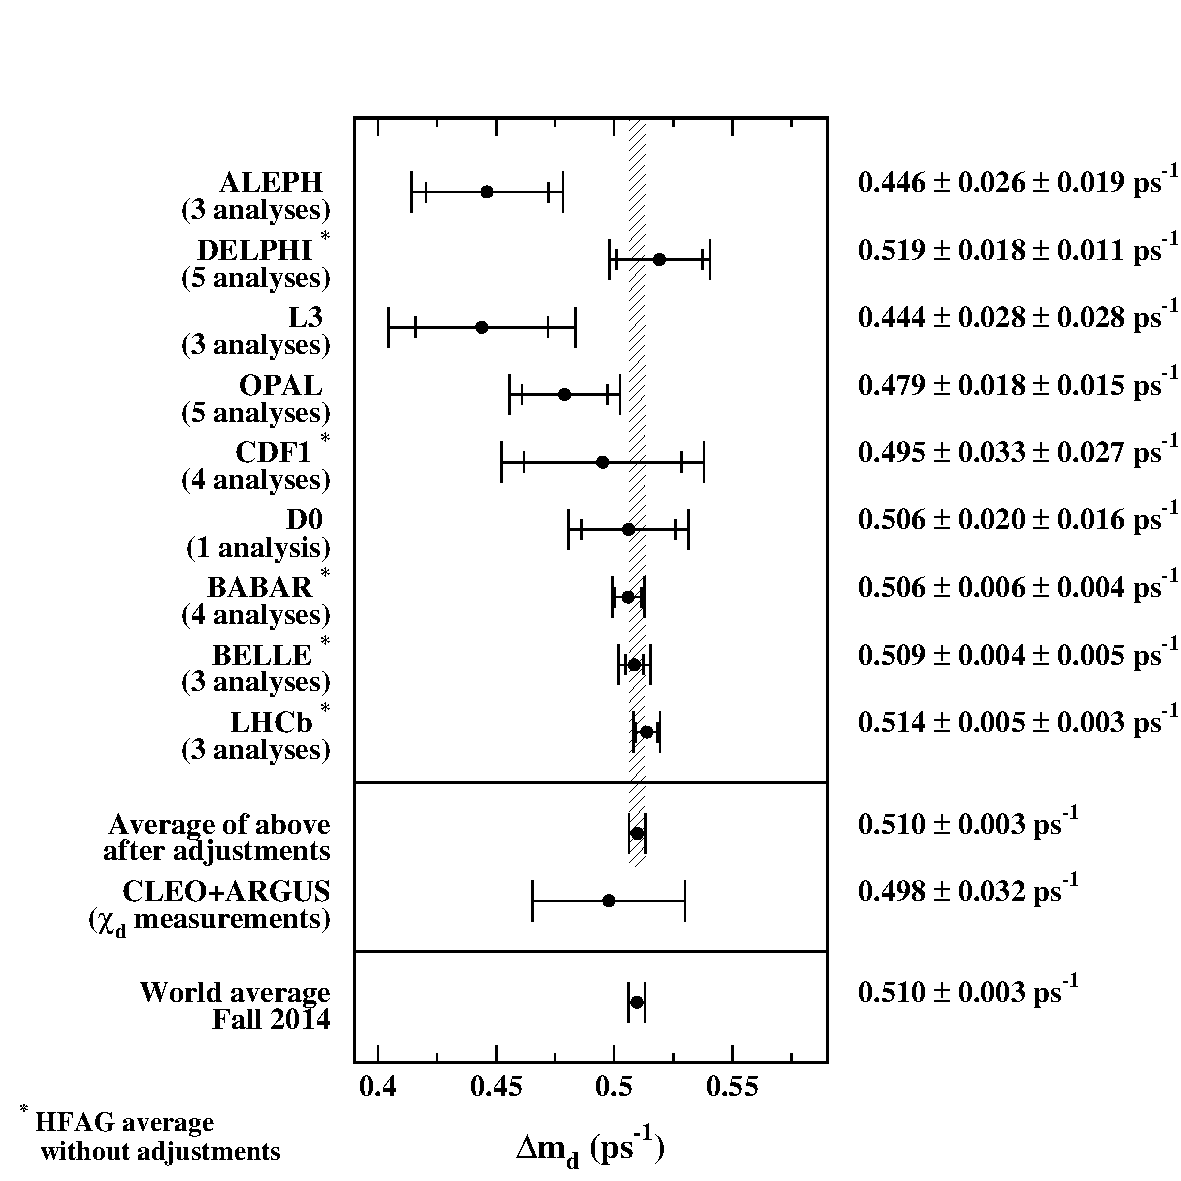
\includegraphics[width=\textwidth]{figures/life_mix/dmd_expt_bw}
\caption{The \Bd--\Bdbar oscillation frequency \dmd as measured by the different experiments. 
The averages quoted for ALEPH, L3 and OPAL are taken from the original publications, while the 
ones for DELPHI, CDF, \babar, \belle and LHCb have been computed from the individual results 
listed in \Table{dmd} without performing any adjustments. The time-integrated measurements 
of \chid from the symmetric \B factory experiments ARGUS and CLEO have been converted 
to a \dmd value using $\tau(\Bd)=\hfagTAUBD$. The two global averages have been obtained 
after adjustments of all the individual \dmd results of \Table{dmd} (see text).}
\labf{dmd}
\end{center}
\end{figure}

The \Bd mixing averages given in \Eqss{dmd}{chid}
and the \b-hadron fractions of \Table{fractions} have been obtained in a fully 
consistent way, taking into account the fact that the fractions are computed using 
the \chid value of \Eq{chid} and that many individual measurements of \dmd
at high energy depend on the assumed values for the \b-hadron fractions.
Furthermore, this set of averages is consistent with the lifetime averages 
of \Sec{lifetimes}.

\begin{table}
\caption{Simultaneous measurements of \dmd and $\tau(\Bd)$, and their average.
The \belle analysis also 
measures $\tau(\Bu)$ at the same time, but it is converted here into a two-dimensional measurement 
of \dmd and $\tau(\Bd)$, for an assumed value of $\tau(\Bu)$. 
The first quoted error on the measurements is statistical
and the second one systematic; in the case of adjusted measurements, the 
latter includes a contribution obtained from the variation of $\tau(\Bu)$ or 
$\tau(\Bu)/\tau(\Bd)$ in the indicated range. Units are\invps\ for \dmd
and\unit{ps} for lifetimes. 
The three different values of $\rho(\dmd,\tau(\Bd))$ correspond 
to the statistical, systematic and total correlation coefficients
between the adjusted measurements of \dmd and $\tau(\Bd)$.}
\labt{dmd2D}
\begin{center}
\begin{tabular}{@{}r@{~}c@{}c@{}c@{~}c@{}c@{}c@{~}c@{}c@{}c@{\hspace{0ex}}c@{}}
\hline
Exp.\ \& Ref.
& \multicolumn{3}{c}{Measured \dmd}   
& \multicolumn{3}{c}{Measured $\tau(\Bd)$}   
& \multicolumn{3}{c}{Measured $\tau(\Bu)$}   
&  Assumed $\tau(\Bu)$ \\
\hline
\babar \cite{Aubert:2002sh}  %{BABAR_dmd_dstarlnu}
      & $0.492$ & $\pm 0.018$ & $\pm 0.013$ 
      & $1.523$ & $\pm 0.024$ & $\pm 0.022$ 
      & \multicolumn{3}{c}{---}
      & $(1.083\pm 0.017)\tau(\Bd)$ \\  
\babar \cite{Aubert:2005kf}  %{BABAR_dmd_preliminary}
      & $0.511$ & $\pm 0.007$ & $^{+0.007}_{-0.006}$ 
      & $1.504$ & $\pm 0.013$ & $^{+0.018}_{-0.013}$
      & \multicolumn{3}{c}{---}
      & $1.671\pm 0.018$ \\  
\belle \cite{Abe:2004mz}  %{BELLE_dmd_full_dstarlnu}
      & $0.511$ & $\pm 0.005$ & $\pm 0.006$
      & $1.534$ & $\pm 0.008$ & $\pm 0.010$
      & $1.635$ & $\pm 0.011$ & $\pm 0.011$
      & --- \\  
\cline{2-10}
& \multicolumn{3}{c}{Adjusted \dmd}   
& \multicolumn{3}{c}{Adjusted $\tau(\Bd)$}   
& \multicolumn{3}{c}{$\rho(\dmd,\Bd)$} 
&  Assumed $\tau(\Bu)$ \\
%----------------------------------------------------------------------------------------
% Numbers below (second part of the table) updated by OS on Mar 23, 2010 based on
% http://lepbosc.web.cern.ch/LEPBOSC/combined_results/mar21/2D/dmd_taubd.results 
%----------------------------------------------------------------------------------------
\cline{2-10}
\babar \cite{Aubert:2002sh}  
      & $0.492$ & $\pm 0.018$ & $\pm 0.013$  % updated Mar 25, 2010
      & $1.523$ & $\pm 0.024$ & $\pm 0.022$  % updated Mar 25, 2010
      & $-0.22$ & $+0.71$ & $+0.16$ % rho_stat,syst,tot % updated Mar 25, 2010
      & $(\hfagRTAUBUval$$\hfagRTAUBUerr)\tau(\Bd)$ \\  
\babar \cite{Aubert:2005kf} 
      & $0.512$ & $\pm 0.007$ & $\pm 0.007$  % updated Mar 25, 2010
      & $1.506$ & $\pm 0.013$ & $\pm 0.018$ % updated Mar 25, 2010
      & $+0.01$ & $-0.85$ & $-0.48$ % rho_stat,syst,tot % updated Mar 25, 2010
      & $\hfagTAUBUval$$\hfagTAUBUerr$ \\  
\belle \cite{Abe:2004mz}  %{BELLE_dmd_full_dstarlnu}
      & $0.511$ & $\pm 0.005$ & $\pm 0.006$ % updated Mar 25, 2010
      & $1.535$ & $\pm 0.008$ & $\pm 0.011$ % updated Mar 25, 2010
      & $-0.27$ & $-0.14$ & $-0.19$ % rho_stat,syst,tot % updated Mar 25, 2010
      & $\hfagTAUBUval$$\hfagTAUBUerr$ \\  
\hline
\multicolumn{1}{l}{Average} 
      & \hfagDMDTWODval   & \hfagDMDTWODsta   & \hfagDMDTWODsys
      & \hfagTAUBDTWODval & \hfagTAUBDTWODsta & \hfagTAUBDTWODsys
      & \hfagRHOstaDMDTAUBD & \hfagRHOsysDMDTAUBD & \hfagRHODMDTAUBD % rho_stat,syst,tot
      & $\hfagTAUBUval$$\hfagTAUBUerr$ \\  
\hline 
\end{tabular}
\end{center}
\end{table}
\begin{figure}
\begin{center}
\vspace{-0.5cm}
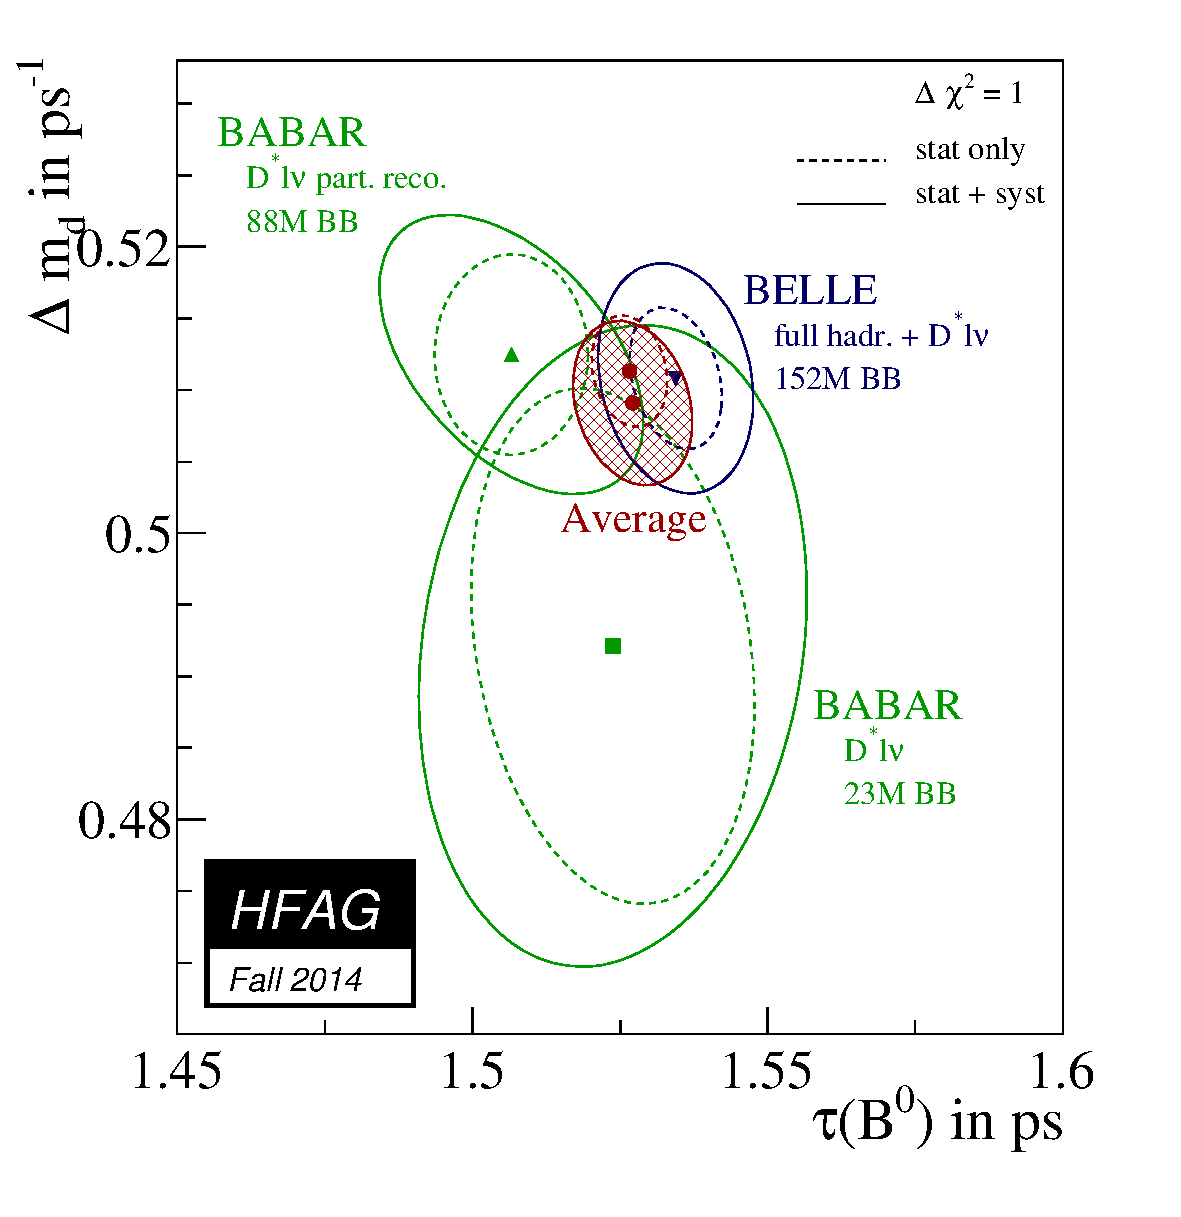
\includegraphics[width=0.6\textwidth]{figures/life_mix/dmd_taubd}
\vspace{-0.5cm}
\caption{Simultaneous measurements of
\dmd and $\tau(\Bd)$~\cite{Aubert:2002sh,Aubert:2005kf,Abe:2004mz}, 
after adjustment to a common set of parameters (see text). 
Statistical and total uncertainties are represented as dashed and
solid contours respectively.
The average of the three measurements
is indicated by a hatched ellipse.}
\labf{dmd2D}
\end{center}
\end{figure}

It should be noted that the most recent (and precise) analyses at the 
asymmetric \B factories measure \dmd
as a result of a multi-dimensional fit. 
Two \babar analyses~\cite{Aubert:2002sh,Aubert:2005kf},  
based on fully and partially reconstructed $\Bd \to D^*\ell\nu$ decays
respectively, 
extract simultaneously \dmd and $\tau(\Bd)$
while the latest \belle analysis~\cite{Abe:2004mz},  %-{BELLE_dmd_full_dstarlnu}, 
based on fully reconstructed hadronic \Bd decays and $\Bd \to D^*\ell\nu$ decays, 
extracts simultaneously \dmd, $\tau(\Bd)$ and $\tau(\Bu)$.
The measurements of \dmd and $\tau(\Bd)$ of these three analyses 
are displayed in \Table{dmd2D} and in \Fig{dmd2D}. Their two-dimensional average, 
taking into account all statistical and systematic correlations, and expressed
at $\tau(\Bu)=\hfagTAUBU$, is
\begin{equation}
\left.
\begin{array}{r@{}l}
\dmd = \hfagDMDTWODnounit & \invps \\
\tau(\Bd) = \hfagTAUBDTWODnounit & \ps
\end{array}
\right\}
~\mbox{with a total correlation of \hfagRHODMDTAUBD.}
\end{equation}

%------------------------------------------------
\mysubsubsection{\Bs mixing parameters \DGs and \dms}
%\mysubsubsection{Mass and decay width differences \dms and \DGs}
%------------------------------------------------
\labs{DGs} \labs{dms}

%%%%%%%%%%%%%%%%%%%%%%%%%%%%%%%%%%%%%%%%%%%%%%%%
%
% This is file life_mix_dgs.tex containing
% the subsection about the 
% decay width difference in the Bs system
%
%%%%%%%%%%%%%%%%%%%%%%%%%%%%%%%%%%%%%%%%%%%%%%%
%

%---------------------------------------------
%\subsubsubsection{Decay width difference \DGs}
%---------------------------------------------

%%%\noindent
%%%\fbox{\parbox{\textwidth}{{\bf WARNING}: Several new results became available but are not yet included in the averages, plots, tables and discussion of this paragraph. These include:
%%%\newline$\bullet$ a finalized version of the analysis described in note ATLAS-CONF-2013-039~\cite{Aad:2014cqa,*Aad:2012kba_cont}; 
%%%\newline$\bullet$ a preliminary analysis from CMS~\cite{CMS-PAS-BPH-13-012};
%%%\newline$\bullet$ a new $\phi_s$ result with $B^0_s\to\jpsi K^+K^-$ from LHCb~\cite{LHCB-PAPER-2014-059,*Aaij:2013oba_supersede2};
%%%}}
%%%\marginpar{XXX}

Definitions and an introduction to \DGs have been given in \Sec{taubs}.
Neglecting \CP violation, the mass eigenstates are
also \CP eigenstates, with the short-lived state being
\CP-even and the long-lived state being \CP-odd.
%
% OL replaces the following by OS PDG2012 section
%
%% Information on \DGs can be obtained by studying the proper time 
%% distribution of untagged data samples enriched in 
%% \Bs mesons~\cite{Hartkorn:1999ga}.
%% In the case of an inclusive \Bs selection~\cite{Acciarri:1998uv} or a semileptonic 
%% \Bs decay selection~\cite{Abreu:2000sh,Abe:1998cj,Abazov:2006cb}, 
%% both the short- and long-lived
%% components are present, and the proper time distribution is a superposition 
%% of two exponentials with decay constants 
%% $\Gs\pm\DGs/2$.
%% In principle, this provides sensitivity to both \Gs and 
%% $(\DGGs)^2$. Ignoring \DGs and fitting for 
%% a single exponential leads to an estimate of \Gs with a 
%% relative bias proportional to $(\DGGs)^2$. 
%% An alternative approach, which is directly sensitive to first order in \DGGs, 
%% is to determine the lifetime of \Bs candidates decaying to \CP
%% eigenstates; measurements exist for 
%% \particle{\Bs\to \jpsi\phi}~\cite{Abe:1997bd,CDFnote8524:2007,*CDFnote8524:2007_cont,Abazov:2004ce} and
%% \particle{\Bs\to D_s^{(*)+} D_s^{(*)-}}, discussed later, which are 
%% mostly \CP-even states~\cite{Aleksan:1993qp}.
%% % RvK
%% However, later, more sophisticated,
%% time-dependent angular analyses of \particle{\Bs\to \jpsi\phi} 
%% allow the simultaneous extraction of \DGs and the \CP-even and \CP-odd 
%% amplitudes~\cite{CDF:2011af,*Aaltonen:2007he_mod,*Aaltonen:2007gf_mod,Abazov:2011ry,*Abazov_mod:2008fj,*Abazov:2007tx_mod_cont}.
%% Flavour tagging the \Bs (or $\bar{B}^0_s$)
%% that subsequently decays to \particle{\jpsi\phi}
%% allows for a more effective
%% extraction of the weak mixing phase as discussed later.
%% % The CDF analysis~\cite{Aaltonen:2007gf} that does not employ flavour tagging
%% % under the assumption of no \CP violation provides a better measurement
%% % of \DGs and is used here, while the CDF analysis~\cite{Aaltonen:2007he}
%% % that does use flavour tagging is used as an input for determining
%% % an average weak mixing phase in the next subsection.
%% Both the CDF and  \dzero flavour-tagged 
%% \particle{\Bs\to \jpsi\phi} analyses~\cite{CDF:2011af,*Aaltonen:2007he_mod,*Aaltonen:2007gf_mod,Abazov:2011ry,*Abazov_mod:2008fj,*Abazov:2007tx_mod_cont} present results first
%% assuming the very small SM value of mixing-induced 
%% \CP violation in the \Bs system
%% (effectively zero compared to current experimental resolution)
%% used in the averaging of \DGs, and then 
%% also allowing for large \CP violation, used for determining
%% an average weak mixing phase in the next subsection.
%% %An estimate of \DGGs
%% %has also been obtained directly from a measurement of the 
%% %\particle{\Bs\to D_s^{(*)+} D_s^{(*)-}} branching ratio~\cite{Barate:2000kd}, 
%% %under the assumption that 
%% %these decays account for all the \CP-even final states 
%% %(however, no systematic uncertainty due to this assumption is given, so 
%% %the average quoted below will not include this estimate).

%% %RvK 1 Feb. 07, move ALEPH measurements from this table to later subsection
%% \begin{table}
%% \caption{Experimental constraints on \DGGs from lifetime 
%% and $B_s \to \jpsi \phi$ analyses,
%% assuming no (or very small SM) \CP violation.
%% The upper limits,
%% which have been obtained by the working group, are quoted at the \CL{95}.}
%% \labt{dgammat}
%% \begin{center}
%% \begin{tabular}{l|c|c|c}
%% \hline
%% Experiment & Method            & $\Delta \Gs/\Gs$ & Ref.  \\
%% \hline
%% L3         & lifetime of inclusive \b-sample              
%%            & $<0.67$   & \cite{Acciarri:1998uv}      \\
%% DELPHI     & $\Bsb\to D_s^+\ell^- \overline{\nu_{\ell}} X$, lifetime
%% 	   & $<0.46$   & \cite{Abreu:2000sh} \\
%% %ALEPH      & $\Bs\to\phi\phi X$ , 
%% %	     \BR{\Bs \to D_s^{(*)+} D_s^{(*)-}}
%% %	   & $0.26^{+0.30}_{-0.15}$ & \cite{Barate:2000kd} \\
%% %ALEPH      & $\Bs\to\phi\phi X$, lifetime 
%% %           & $0.45^{+0.80}_{-0.49}$ & \cite{Barate:2000kd}\\
%% %CDF~\cite{CDF-Dsl}        & $\Bsb \to D_s^+ \ell^- \overline{\nu_{\ell}}  X$ &
%% %$\tbssemi=(1.36\pm0.09^{+0.06}_{-0.05})$~ps  & $<0.83$ \\
%% DELPHI     & $\Bsb \to D_s^+$ hadron, lifetime
%%            & $<0.69$ & \cite{Abreu:2000ev}   \\
%% CDF1       & $\Bs \to \jpsi\phi$, lifetime
%% 	   & $0.33^{+0.45}_{-0.42}$ & \cite{Abe:1997bd} \\ \hline
%% 	   &                   & $ \DGs$  \\ \hline
%% % RvK July 2008, update to CDF arXiv:0712.2348 analysis; note that
%% % this is the one optimized for Delta(Gamma_s) assuming phi_s = 0
%% % RvK June 2010, update to preliminary 2.8 fb-1 CDF note
%% CDF2       & $\Bs \to \jpsi\phi$, time-dependent angular analysis
%%            & $0.02{\pm 0.05}{\pm 0.01\invps}$ & \cite{CDF:2011af,*Aaltonen:2007he_mod,*Aaltonen:2007gf_mod} \\ 
%% % RvK July 2008, update to D0  arXiv:/0802.2255 [hep-ex]
%% \dzero     & $\Bs \to \jpsi\phi$, time-dependent angular analysis
%%            & $0.14{\pm 0.07\invps}$ & \cite{Abazov:2011ry,*Abazov_mod:2008fj,*Abazov:2007tx_mod_cont} \\
%% 	 \hline
%% %%% \multicolumn{4}{l}{$^p$ \footnotesize Preliminary}
%% 	 \end{tabular}
%% 	 \end{center}
%% 	 \end{table}
%
%

%% Results of the combination are shown as the one-sigma contour
%% labeled ``Direct" in both plots of \Fig{DGs}.  Transformation
%% of variables from $(1/\Gs,\,\DGs)$ space to other pairs
%% of variables such as $(1/\Gs,\,\DGGs)$ and 
%% $(\tau_{\rm L} = 1/\Gamma_{\rm L},\,\tau_{\rm H} = 1/\Gamma_{\rm H})$
%% are also made.
%% The resulting one-sigma contour for the latter is shown in
%% \Fig{DGs}(b). 

The best sensitivity to \DGs is currently achieved 
by the recent time-dependent measurements
of the $\Bs\to\jpsi\phi$ (or more generally $\Bs\to\jpsi K^+K^-$) decay rates performed at
CDF~\cite{Aaltonen:2012ie,*CDF:2011af,*Aaltonen:2007he_mod,*Aaltonen:2007gf_mod},
\dzero~\cite{Abazov:2011ry,*Abazov_mod:2008fj,*Abazov:2007tx_mod_cont}, 
ATLAS~\cite{Aad:2014cqa,*Aad:2012kba_cont}, CMS~\cite{CMS-PAS-BPH-11-006,CMS-PAS-BPH-13-012}
and LHCb~\cite{LHCB-PAPER-2014-059,*Aaij:2013oba_supersede2},
where the \CP-even and \CP-odd
amplitudes are statistically separated through a full angular analysis
(see last two columns of \Table{phisDGsGs}). 
%OS% In addition, 
%OS% LHCb~\cite{Aaij:2013oba,*LHCb:2011aa_mod,*LHCb:2012ad_mod,*LHCb:2011ab_mod,*Aaij:2012nta_mod}
%OS% has analyzed $\Bs\to\jpsi \pi^+\pi^-$ decays, for which no angular analysis is needed. 
With the exception of the first CMS analysis~\cite{CMS-PAS-BPH-11-006},
these studies use both untagged and tagged \Bs\ candidates and 
are optimized for the measurement of the \CP-violating 
phase \phiccbars, defined later in \Sec{phasebs}.
The LHCb collaboration analyzed the $\Bs \to \jpsi K^+K^-$
decay, considering that the $K^+K^-$ system can be in a $P$-wave or $S$-wave state, 
and measured the dependence of the strong phase difference between the 
$P$-wave and $S$-wave amplitudes as a function of the $K^+K^-$ invariant
mass~\cite{Aaij:2012eq}. 
This allowed, for the first time, the unambiguous determination of the sign of 
$\DGs$, which was found to be positive at the $4.7\,\sigma$ level and the
following averages present only the $\DGs > 0$ solutions.

%wrong% The combined fit procedure used to extract simultaneously \DGs\ and \phiccbars
%wrong% is described in \Sec{phasebs}. 
%wrong% The results, displayed as the red contours labelled ``$\Bs \to \jpsi\phi$ measurements'' in the 
%wrong% plots of \Fig{DGs}, are given in the first column of numbers of \Table{tabtauLH}.
%wrong% In those averages, the correlation between \DGs and \Gs has been neglected. 

The available results~\cite{Aaltonen:2012ie,*CDF:2011af,*Aaltonen:2007he_mod,*Aaltonen:2007gf_mod,Abazov:2011ry,*Abazov_mod:2008fj,*Abazov:2007tx_mod_cont,Aad:2014cqa,*Aad:2012kba_cont,CMS-PAS-BPH-11-006,CMS-PAS-BPH-13-012,LHCB-PAPER-2014-059,*Aaij:2013oba_supersede2}
are shown in \Table{GsDGs}. They are combined, taking into account, in each analysis, the correlation between \DGs and \Gs.
The results, displayed as the red contours labelled ``$\Bs \to \jpsi (\phi/KK)$ measurements'' in the
plots of \Fig{DGs}, are given in the first column of numbers of \Table{tabtauLH}.

\begin{table}
\caption{Measurements of \DGs and \Gs using
$\Bs\to\jpsi\phi$ and $\Bs\to\jpsi K^+K^-$ decays.
Only the solution with $\DGs > 0$ is shown, since the two-fold ambiguity has been
resolved in \Ref{Aaij:2012eq}. The first error is due to 
statistics, the second one to systematics. The last line gives our average.}
\labt{GsDGs}
\begin{center}
%\begin{tabular}{l@{\,}l@{\,}l@{\,}|@{\,}l@{\,}|@{\,}l@{\,}|@{\,}l} 
\begin{tabular}{llrlll} 
\hline
% Exp.\ & Mode & Dataset & \multicolumn{1}{c@{\,}|@{\,}}{\phiccbars}
%                      & \multicolumn{1}{c@{}}{\DGs (\!\!\invps)} & Ref.\ \\
Exp.\ & Mode & Dataset
      & \multicolumn{1}{c}{\DGs (\!\!\invps)}
      & \multicolumn{1}{c}{\Gs  (\!\!\invps)}
      & Ref.\ \\
\hline
CDF    & $\jpsi\phi$ & $9.6\invfb$
       & $0.068\pm0.026\pm0.009$
       % syst error was +-0.007 instead of +-0.009 in CDF note 10778
       % & $0.6545\pm0.0081\pm0.0039$
       & $0.654\pm0.008\pm0.004$ % quoted in paper as tau(Bs) = 1/Gamma_s = 1.528 +-0.019 +-0.009
% 1./1.528 = 0.6544502617801047, 0.019/1.528**2 = 0.008137797757736905, 0.009//1.528**2 = 0.003854746306296428
       & \cite{Aaltonen:2012ie,*CDF:2011af,*Aaltonen:2007he_mod,*Aaltonen:2007gf_mod} \\
\dzero & $\jpsi\phi$ & $8.0\invfb$
       & $0.163^{+0.065}_{-0.064}$ 
       & $0.693^{+0.018}_{-0.017}$
       & \cite{Abazov:2011ry,*Abazov_mod:2008fj,*Abazov:2007tx_mod_cont} \\
ATLAS  & $\jpsi\phi$ & $4.9\invfb$
       & $0.053 \pm0.021 \pm0.010$
       & $0.677 \pm0.007 \pm0.004$
       & \cite{Aad:2014cqa,*Aad:2012kba_cont} \\
CMS    & $\jpsi\phi$ & $5.0\invfb$ 
       & $0.048\pm0.024\pm0.003$
       & $0.655\pm0.008\pm0.003$
%%% the CMS note CMS-PAS-BPH-11-006 quotes a "mean Bs lifetime" of
%%%    ctau = 458.0 +-5.9 +-2.2 microns = 1.528 +-0.020 +-0.007 ps
%%%    corresponding to Gamma_s = 0.6546 +-0.0084 +-0.0031 ps-1
       & \cite{CMS-PAS-BPH-11-006}$^p$ \\
CMS    & $\jpsi\phi$ & $20\invfb$ 
       & $0.096\pm0.014\pm0.007$
       & $0.670 \pm0.004 \pm0.005$
%%% the CMS note CMS-PAS-BPH-13-012 quotes a "mean Bs lifetime" of
%%%    ctau = 447.3 +-3.0 +-3.5 microns = 1.492 +-0.010 +-0.012 ps
%%%    corresponding to Gamma_s = 0.6702 +-0.0045 +-0.0052 ps-1
       & \cite{CMS-PAS-BPH-13-012}$^p$ \\
LHCb   & $\jpsi KK$ & $3.0\invfb$
       & $0.0805\pm0.0091\pm0.0033$
       & $0.6603\pm0.0027\pm0.0015$
       & \cite{LHCB-PAPER-2014-059,*Aaij:2013oba_supersede2} \\
\hline
\multicolumn{3}{l}{All combined} & \hfagDGSnounit & \hfagGSnounit & \\ 
\hline
\multicolumn{6}{l}{$^p$ {\footnotesize Preliminary.}}
\end{tabular}
\end{center}
\end{table}

\begin{figure}
\begin{center}
\epsfig{figure=figures/life_mix/hfag_Fall2014_DGsGs_tauLtauH.pdf,width=0.99\textwidth}
\caption{Contours of $\Delta \ln L = 0.5$ (39\% CL for the enclosed 2D regions, 68\% CL for the bands)
shown in the $(\Gs,\,\DGs)$ plane on the left
and in the $(1/\Gamma_{\rm L},\,1/\Gamma_{\rm H})$ plane on the right. 
The average of all the $\Bs \to \jpsi\phi$ and $\Bs\to \jpsi K^+K^-$ 
% and $\jpsi\pi^+\pi^-$
results is shown as the red contour,
and the constraints given by the effective lifetime measurements of
\Bs\ to flavour-specific, pure \CP-odd and pure \CP-even final states
are shown as the blue, green and purple bands, 
respectively. The average taking all constraints into account is shown as the gray-filled contour.
The yellow band is a theory prediction
$\DGs = 0.087 \pm 0.021~\hbox{ps}^{-1}$~\cite{Lenz:2011ti,*Lenz:2006hd}
that assumes no new physics in \Bs\ mixing.}
% ,!!!!!!!!TO BE UPDATED !!!!!!\DGs combination results with one-sigma contours
% ($\Delta\log\mathcal{L} = 0.5$) shown for (a) \DGs versus
% $\bar{\tau}(\Bs) = 1/\Gs$  and (b)
% $\tau_{\rm H} = 1/\Gamma_{\rm H}$ versus $\tau_{\rm L} = 1/\Gamma_{\rm L}$.
% The red contours labeled ``Direct" are the result of the combination of
% last two measurements of \Table{dgammat}, the blue bands are the one-sigma
% contours due to the world average of flavour-specific 
% \Bs lifetime measurements,
% the green bands are the one-sigma contour of the $\Bs \to K^+K^-$ 
% lifetime measurement, 
% and the solid and dashed-outlined shaded regions result using
% the combination constraints described in the text.}
\labf{DGs}
\end{center}
\end{figure}

\begin{table}
\caption{Averages of \DGs, $\Gs$ and related quantities, obtained from
$\Bs\to\jpsi\phi$ and $Bs\to\jpsi K^+K^-$ alone (first column),
adding the constraints from the effective lifetimes measured in pure \CP modes
%OL2014 $\Bs\to K^+ K^-, \, D_s^+D_s^-, \, \jpsi f_0(980), \jpsi K_{\rm S}^0$ (second column),
$\Bs\to D_s^+D_s^-$ and $\Bs \to \jpsi f_0(980), \jpsi \pi^+\pi^-$ (second column),
and adding the constraint from the effective lifetime measured in flavour-specific modes
$\Bs\to D_s^-\ell^+\nu X, \, D_s^-\pi^+, \, D_s^-D^+$ (third column, recommended world averages).}
\labt{tabtauLH}
\begin{center}
\begin{tabular}{c|c|c|c}
\hline
% & $\jpsi hh$
% & $\jpsi hh, \mbox{\CP-even}, \mbox{\CP-odd}$
% & $\jpsi hh, \mbox{\CP-even}, \mbox{\CP-odd}, \mbox{flavour-specific}$ \\
& $\Bs\to\jpsi KK$ modes & $\Bs\to\jpsi KK$ modes & $\Bs\to\jpsi KK$ modes \\
& only (see \Table{GsDGs}) & + pure \CP modes & + pure \CP modes \\
&                          &                  & + flavour-specific modes \\
\hline
\Gs                & \hfagGS        &  \hfagGSCO        &  \hfagGSCON        \\
$1/\Gs$            & \hfagTAUBSMEAN &  \hfagTAUBSMEANCO &  \hfagTAUBSMEANCON \\
$1/\Gamma_{\rm L}$ & \hfagTAUBSL    &  \hfagTAUBSLCO    &  \hfagTAUBSLCON    \\
$1/\Gamma_{\rm H}$ & \hfagTAUBSH    &  \hfagTAUBSHCO    &  \hfagTAUBSHCON    \\
\DGs               & \hfagDGS       &  \hfagDGSCO       &  \hfagDGSCON       \\
\DGs/\Gs           & \hfagDGSGS     &  \hfagDGSGSCO     &  \hfagDGSGSCON     \\
$\rho(\Gs,\DGs)$   & \hfagRHOGSDGS  &  \hfagRHOGSDGSCO  &  \hfagRHOGSDGSCON  \\
\hline
\end{tabular}
\end{center}
\end{table}

%The positive sign of $\DGs$ is due to the constraint applied 
%on $\phi_s$. In absence of such constraint, there would be two 
%mirror solutions related by the transformation
%$(\DGs, \phi_s)  \to (-\DGs, \pi-\phi_s)$.

An alternative approach, which is directly sensitive to first order in 
$\DGs/\Gs$, 
is to determine the effective lifetime of untagged \Bs\ candidates
decaying to %fairly
pure \CP eigenstates; we use here measurements with
%OL 2014 $\Bs \to K^+K^-$~\cite{Aaij:2011kn,Aaij:2014fia,*Aaij:2012ns_cont}%
%\footnote{An old unpublished measurement of the $\Bs \to K^+ K^-$
%effective lifetime by CDF~\cite{Tonelli:2006np} is no longer considered.},
$\Bs \to D_s^+D_s^-$~\cite{Aaij:2013bvd}, 
$\Bs \to \jpsi f_0(980)$~\cite{Aaltonen:2011nk}
and $\Bs\to \jpsi \pi^+\pi^-$~\cite{Aaij:2013oba,*LHCb:2011aa_mod,*LHCb:2012ad_mod,*LHCb:2011ab_mod,*Aaij:2012nta_mod} decays.
% OL2014 and $\Bs \to \jpsi K_{\rm S}^0$~\cite{Aaij:2013eia}.
The precise extraction of $1/\Gs$ and $\DGs$
from such measurements, discussed in detail in \Ref{Fleischer:2011cw}, 
requires additional information 
in the form of theoretical assumptions or
external inputs on weak phases and hadronic parameters. 
If $f$ designates a final state in which both \Bs and \Bsbar can decay,
the ratio of the effective \Bs lifetime decaying to $f$ relative to the mean
\Bs lifetime is~\cite{Fleischer:2011cw}%
\footnote{The definition of $A_f^{\DG}$ given in \Eq{ADG} has the sign opposite to that given in \Ref{Fleischer:2011cw}.}
\begin{equation}
  \frac{\tau_{\rm single}(\Bs \to f)}{\tau(\Bs)} = \frac{1}{1-y_s^2} \left[ \frac{1 - 2A_f^{\DG} y_s + y_s^2}{1 - A_f^{\DG} y_s}\right ] \,,
%   = 1 - A_f^{\DG} y_s + 2 y_s^2\left [ 2 - (A_f^{\DG})^2 \right ] + \mathcal{O}(y_s^3),
\labe{tauf_fleisch}
\end{equation}
where
\begin{equation}
A_f^{\DG} = -\frac{2 \Re(\lambda_f)} {1+|\lambda_f|^2} \,.
\labe{ADG}
\end{equation}
To include the measurements of the effective
%OL2014 $\Bs\to K^+ K^-$ (\CP-even),
$\Bs \to D_s^+D_s^-$ (\CP-even), $\Bs \to \jpsi f_0(980)$ (\CP-odd) and
$\Bs \to \jpsi\pi^+\pi^-$ (\CP-odd) 
% $\Bs \to \jpsi K_{\rm S}^0$ (\CP-odd)
lifetimes as constraints in the \DGs fit,\footnote{%
The effective lifetimes measured in $\Bs\to K^+ K^-$ (mostly \CP-even) and  $\Bs \to \jpsi K_{\rm S}^0$ (mostly CP-odd) are not used because we can not quantify the penguin contributions in those modes.}
we neglect sub-leading penguin contributions and possible direct \CP violation. 
Explicitly, in \Eq{ADG}, we set
$A_{\mbox{\scriptsize \CP-even}}^{\DG} = \cos \phiccbars$
and $A_{\mbox{\scriptsize \CP-odd}}^{\DG} = -\cos \phiccbars$.
Given the small value of $\phiccbars$, we have, to first order in $y_s$:
\begin{eqnarray}
\tau_{\rm single}(\Bs \to \mbox{\CP-even})
& \approx & \frac{1}{\Gamma_{\rm L}} \left(1 + \frac{(\phiccbars)^2 y_s}{2} \right) \,,
\labe{tau_KK_approx}
\\
\tau_{\rm single}(\Bs \to \mbox{\CP-odd})
& \approx & \frac{1}{\Gamma_{\rm H}} \left(1 - \frac{(\phiccbars)^2 y_s}{2} \right) \,.
\labe{tau_Jpsif0_approx}
\end{eqnarray}
The numerical inputs are taken from \Eqss{tau_KK}{tau_Jpsif0}
%OL2014 \footnote{The LHCb effective lifetime measurement obtained with 
%$\Bs \to\jpsi\pi^+\pi^-$ decays~\cite{Aaij:2013oba,*LHCb:2011aa_mod,*LHCb:2012ad_mod,*LHCb:2011ab_mod,*Aaij:2012nta_mod}
%is first removed from the average of \Eq{tau_Jpsif0}, 
%yielding 
%$\tau_{\rm single}(\Bs \to \mbox{\CP-odd}) = \hfagTAUBSLONGCON$, because this 
%information is already contained in the $\Bs \to \jpsi hh$ analysis.}
and the resulting averages, combined with the $\Bs\to\jpsi K^+K^-$ information,
are indicated in the second column of numbers of \Table{tabtauLH}. 
These averages assume $\phiccbars = 0$, which is compatible with
%OS% the central value of
the \phiccbars average presented in \Sec{phasebs}.

Information on \DGs can also be obtained from the study of the
proper time distribution of untagged samples
of flavour-specific \Bs decays~\cite{Hartkorn:1999ga}, where
the flavour (\ie\ \Bs or \Bsbar) at the time of decay can be determined by
the decay products. In such decays,
\eg\ semileptonic \Bs decays, there is
an equal mix of the heavy and light mass eigenstates at time zero.
The proper time distribution is then a superposition 
of two exponential functions with decay constants
$\Gamma_{\rm L,H} = \Gs \pm \DGs/2$.
This provides sensitivity to both $1/\Gs$ and 
$(\DGs/\Gs)^2$. Ignoring \DGs and fitting for 
a single exponential leads to an estimate of \Gs with a 
relative bias proportional to $(\DGs/\Gs)^2$, as shown in \Eq{fslife}. 
Including the constraint from the world-average flavour-specific \Bs 
lifetime, given in \Eq{tau_fs}, leads to the results shown in the last column 
of \Table{tabtauLH}.
% These world averages are the default recommended world averages. 
These world averages are displayed as the gray contours labelled ``Combined'' in the
plots of \Fig{DGs}. 
They correspond to the lifetime averages
$1/\Gs=\hfagTAUBSMEANCON$,
$1/\Gamma_{\rm L}=\hfagTAUBSLCON$,
$1/\Gamma_{\rm H}=\hfagTAUBSHCON$,
and to the decay-width difference
\begin{equation}
\DGs = \hfagDGSCON ~~~~\mbox{and} ~~~~~ \DGs/\Gs = \hfagDGSGSCON \,, 
\labe{DGs_DGsGs}
\end{equation}
which is in good agreement with the Standard Model prediction 
$\DGs = 0.087 \pm 0.021~\hbox{ps}^{-1}$~\cite{Lenz:2011ti,*Lenz:2006hd}.

Independent estimates of $\DGs/\Gs$ obtained from measurements of the 
$\Bs \to D_s^{(*)+} D_s^{(*)-}$ branching fraction~\cite{Barate:2000kd,Esen:2010jq_mod,Abazov:2008ig,*Abazov:2007rb_mod_cont,Abulencia:2007zz}
have not been used,
%OS% \footnote{%
%OS% A new average is being prepared.},
%XXXXX%OS%%Our average is ${\cal B} = \hfagBRDSDS$, from which one would get 
%XXXXX%OS%%$\DGs/\Gs \sim 2{\cal B}/(1-{\cal B}) = \hfagDGSGSBRDSDS$.},
since they are based on the questionable~\cite{Lenz:2011ti,*Lenz:2006hd}
assumption that these decays account for all \CP-even final states.
The results of early lifetime analyses attempting
to measure $\DGs/\Gs$~\cite{Acciarri:1998uv,Abreu:2000sh,Abreu:2000ev,Abe:1997bd}
have not been used either. 

%as the weak phase difference between
%the \Bs--\Bsbar\ mixing
%diagram and the $b \to c\bar{c}s$ tree decay diagram. 
%The Standard Model prediction for $\phi_s$, if Penguin pollution 
%is neglected, is equal to 
%$-2\beta_s = -2\arg(-(V_{ts}^{}V_{tb}^*)/(V_{cs}^{}V_{cb}^*))
%= -0.0367\,^{+0.0014}_{-0.0013}$~\cite{Charles:2011va_mod}.


%A combination of
%the published % $\hbox{\Bs} \to \jpsi \phi$ 
%analyses~\cite{CDF:2011af,*Aaltonen:2007he_mod,*Aaltonen:2007gf_mod,Abazov:2011ry,*Abazov_mod:2008fj,*Abazov:2007tx_mod_cont,LHCb:2011aa}, 
%where $\phi_s$ is constrained to the above Standard Model range, 
%and of the flavour-specific lifetime
%measurements~\cite{Buskulic:1996ei,Ackerstaff:1997qi,Abe:1998cj,Abreu:2000sh,Abazov:2006cb,Aaltonen:2011qsa,*Aaltonen:2011qsa_cont}
%yields







% OL> I don't touch the following: I let it for you RickVK

 
%% Measurements quoting \DGGs results from lifetime analyses
%% and \DGs results from $B^0_s \to \jpsi \phi$ analyses
%% under the hypothesis of no (or very small SM) \CP violation
%% are listed in \Table{dgammat}.  
%% There is significant correlation
%% between \DGs and $1/\Gs$. In order to combine these measurements,
%% the two-dimensional log-likelihood for each measurement
%% in the $(1/\Gs,\,\DGs)$ plane is summed and the total
%% normalized with respect to its minimum.  The one-sigma contour (corresponding
%% to 0.5 units of log-likelihood greater than the minimum) and
%% 95\% CL contour are found. 
%% Only the \DGs inputs 
%% from CDF2 and \dzero as indicated in 
%% \Table{dgammat} were used in the combinations below
%% (adding the other ones would not change the results).
%% 
%
%% CDF has very recently made a preliminary
%% update~\cite{CDFnote10778:2012,*CDFnote10778:2012_cont}
%% to their
%% \particle{\Bs \to \jpsi\phi} analysis to an
%% integrated luminosity of 5.2~fb$^{-1}$, and assuming no \CP violation, 
%% find
%% \begin{eqnarray}
%% \DGs &=& 0.075 \pm 0.035 \pm 0.01 \thinspace {\mathrm{ps}}^{-1} \,, \\
%% \bar{\tau}(\Bs) = 1/\Gs &=& 1.530 \pm 0.025 \pm 0.012 \thinspace
%% {\mathrm{ps}} \,. 
%% \end{eqnarray}
%% However, this new update has yet to be included in the following
%% combinations.

%with the exception of the L3~\cite{Acciarri:1998uv} result since the likelihood
%in this case was not available.
%and the 
%ALEPH~\cite{Barate:2000kd} branching ratio result for the reason
%given above.


% Present published data is not precise enough to efficiently constrain 
% both \Gs and \DGGs; since the \Bs and \Bd 
% lifetimes are predicted to be equal within a 
% percent~\cite{Beneke:1996gn,*Keum:1998fd,Gabbiani:2004tp}, an expectation compatible with 
% the current experimental data (see \Table{liferatio}),
% the constraint $\Gs = \Gd$ can also be used to improve the
% extraction of \DGGs.
% Applying the combination procedure of \Ref{Abbaneo:2000ej_mod,*Abbaneo:2001bv_mod_cont}
% on the published results~%
% \cite{Abreu:2000sh,Abe:1998cj,Abe:1997bd,Barate:2000kd,Buskulic:1996ei,Ackerstaff:1997qi}
% yields

%%%%%%%%%%%%%%%%%%%%%%%%%%%%%%%%%%%%%%%%%%%%
%%%%%%%%%%%%%%%%%%%%%%%%%%%%%%%%%%%%%%%%%%%%
%%%%%%%%%%%%%%%%%%%%%%%%%%%%%%%%%%%%%%%%%%%%

% OL>: Rick, please write this as you wish
\comment{


% {\em Results for Fall 2006 \ldots}

% Results of Rick \DGs program:


Numerical results of the combination of the CDF2 and \dzero inputs
of \Table{dgammat} are:
\begin{eqnarray}
\DGGs &=& \hfagDGSGS \,, \\
\DGs &=& \hfagDGS \,, \\
\bar{\tau}(\Bs) = 1/\Gs &=& \hfagTAUBSMEAN \,, \\
% \rho(\DGGs, 1/\DGs) &=& \hfagRHODGSGSTAUBSMEAN \,, \\
1/\Gamma_{\rm L} = \tau_{\rm short} &=& \hfagTAUBSL \,, \\
1/\Gamma_{\rm H} = \tau_{\rm long}  &=& \hfagTAUBSH \,. 
\end{eqnarray}

Flavour-specific lifetime measurements are of an equal mix
of \CP-even and \CP-odd states at time zero, and  
if a single exponential function is used in the likelihood
lifetime fit of such a sample~\cite{Hartkorn:1999ga}, 
\begin{equation}
\tau(\Bs)_{\rm fs} = \frac{1}{\Gs}
\frac{{1+\left(\frac{\DGs}{2\Gs}\right)^2}}{{1-\left(\frac{\DGs}{2\Gs}\right)^2}
} \,.
\labe{fslife_const}
\end{equation}
Using the world average flavour-specific 
lifetime of \Eq{tau_fs} in \Sec{taubs}
the one-sigma blue bands shown in \Fig{DGs} are obtained. 
Higher-order corrections were checked to be negligible in the
combination.

When the flavour-specific lifetime measurements 
are combined with the 
CDF2 and \dzero measurements of \Table{dgammat}, the solid-outline
shaded
regions of \Fig{DGs} are obtained, with numerical results:
\begin{eqnarray}
\DGGs &=& \hfagDGSGSCON \,, \labe{DGGs_ave} \\
\DGs &=& \hfagDGSCON \,, \\
\bar{\tau}(\Bs) = 1/\Gs &=& \hfagTAUBSMEANC \,, \labe{oneoverGs} \\
% \rho(\DGGs, 1/\DGs) &=& \hfagRHODGSGSTAUBSMEANCON \,,  \\
1/\Gamma_{\rm L} = \tau_{\rm short} &=& \hfagTAUBSLCON \,, \\
1/\Gamma_{\rm H} = \tau_{\rm long}  &=& \hfagTAUBSHCON \,. 
\end{eqnarray}
These results can
be compared with the theoretical prediction of 
$\DGs = 0.096 \pm 0.039\invps$
(or $\DGs = 0.088 \pm 0.017\invps$ if there is no new physics in
\dms)~\cite{Lenz:2011ti,*Lenz:2006hd,Beneke:1998sy}.


Measurements of $\BR{B^0_s \to D_s^{(*)+} D_s^{(*)-}}$ can 
also be sensitive to \DGs.
The decay $\Bs \to D_s^{+} D_s^{-}$ is into
a final state that is purely \CP even. 
Under various theoretical assumptions~\cite{Aleksan:1993qp,Dunietz:2000cr}, the
inclusive decay into this plus the excited states
$\Bs \to D_s^{(*)+} D_s^{(*)-}$ is also \CP even
to within 5\%, and 
$\Bs \to D_s^{(*)+} D_s^{(*)-}$ saturates
$\Gs^{\CP \thinspace {\rm even}}$.
Under these assumptions, for no \CP violation, we have: 
\begin{equation}
\DGGs \approx
\frac{2 \BR{\Bs \to D_s^{(*)+} D_s^{(*)-}}}
{1 - \BR{\Bs \to D_s^{(*)+} D_s^{(*)-}}} \,.
\labe{dGsBr}
\end{equation}
However, there are concerns~\cite{Nierste_private:2006} 
that the assumptions needed
for the above are overly restrictive and that the inclusive branching
ratio may be \CP even to only 30\%.
In the application of the constraint as a Gaussian penalty
function, the theoretical uncertainty is dealt with in two ways:
the fraction of the \CP-odd component of the decay~\cite{Dunietz:2000cr} 
is taken
to be a uniform distribution ranging from 0 to 0.05 and
convoluted in the Gaussian, and the fractional uncertainty on the
average measured value is increased in quadrature by 
30\%.

\begin{table}
\caption{Measurements of $\BR{\Bs \to D_s^{(*)+} D_s^{(*)-}}$.}
\labt{dGsBr}
\begin{center}
\begin{tabular}{l|c|c|c}
\hline
Experiment & Method & Value & Ref.  \\
\hline
%May1,2010% \belle         & \Bs-pair production at $\Upsilon(5S)$
%May1,2010%               & $< 0.257$ at 90\% CL & \cite{Drutskoy:2006xc}$^b$  \\
ALEPH         & $\phi$-$\phi$ correlations              
           & $0.115 \pm 0.050^{+0.095}_{-0.045}$  & \cite{Barate:2000kd}$^a$     \\
\dzero        & $D_s \to \phi \pi$, $D_s \to \phi \mu \nu$            
           & $0.035 \pm 0.010 \pm 0.011$  & \cite{Abazov:2008ig,*Abazov:2007rb_mod_cont}$^{~}$ \\
\belle      & full reco.\ in 6 excl.\ $D_s$ modes 
            & $0.0685 ^{+0.0153}_{-0.0130} {}^{+0.0179}_{-0.0180}$ & \cite{Esen:2010jq_mod}$^{~}$ \\
	 \hline
\multicolumn{2}{l}{Average of above 3} &   \hfagBRDSDS  &   \\
      \hline
%May1,2010% \multicolumn{4}{l}{
%May1,2010% $^b$ \footnotesize This limit is for $\Bs \to D_s^{*+} D_s^{*-}$.} \\[-0.5ex]
\multicolumn{4}{l}{
$^a$ \footnotesize The value quoted in this table is half of 
$\BR{\Bs{\rm(short)} \to D_s^{(*)+} D_s^{(*)-}}$
given in \Ref{Barate:2000kd}.} \\[-0.5ex]
\multicolumn{4}{l}{$^{~}$ \footnotesize Before averaging, it has been adjusted the latest values
of \fBs at LEP and \BR{\Ds \to \phi X}.} 
% \\[-0.5ex] \multicolumn{4}{l}{$^p$ \footnotesize Preliminary.} 
\end{tabular}
\end{center}
\end{table}

Measurements for the branching fraction for this
decay channel are shown in \Table{dGsBr}.
Using their average value of \hfagBRDSDS with \Eq{dGsBr} yields
\begin{equation}
\DGGs = \hfagDGSGSBRDSDS \,,
\end{equation}
consistent with the value given in \Eq{DGGs_ave}. 

As described in \Sec{taubs}
and \Eq{tau_CPeven}, the average of the lifetime
measurements with \Bs $\to K^+ K^-$ and
$\Bs \to D_s^{(*)} D_s^{(*)}$ decays
can be used to measure the lifetime
of the \CP-even (or ``light" mass) eigenstate
$\tau(\Bs \to \CP\mbox{-even}) = \tau_L = 1/\Gamma_{\rm L} =
\hfagTAUBSSHORT$. These decays are assumed to be 100\% \CP even, with
a 5\% theoretical uncertainty on this assumption added in quadrature
for the combination.

%end-2009% When the constraint due this \CP-even lifetime and
%end-2009% the $\BR{B^0_s \to D_s^{(*)+} D_s^{(*)-}}$
%end-2009% branching fraction are
%end-2009% added to the previous ones,
%end-2009% the dashed-outline
%end-2009% shaded
%end-2009% regions of \Fig{DGs} are obtained, with numerical results:

CDF has also measured the exclusive branching fraction 
$\BR{B^0_s \to D^+_s D^-_s} = 
(9.4^{+4.4}_{-4.2}) \times 10^{-3}$~\cite{Abulencia:2007zz}, and
they use this to set a lower bound of
$\DGs^{\CP}/\Gs \geq 0.012$ at \CL{95} (since
on its own it does not saturate the \CP-even states).

} % end comment

 

%--------------------------------------
%\subsubsubsection{\boldmath Mass difference \dms}
%--------------------------------------

The strength of \Bs mixing is known to be large since more than 20 years. 
Indeed the time-integrated measurements of \chibar (see \Sec{chibar}),
when compared to our knowledge
of \chid and the \b-hadron fractions, indicated that 
\chis should be close to its maximal possible value of $1/2$.
Many searches of the time dependence of this mixing 
were performed by ALEPH~\cite{Heister:2002gk},
CDF (Run~I)~\cite{Abe:1998qj},
DELPHI~\cite{Abreu:2000sh,Abreu:2000ev,Abdallah:2002mr,Abdallah:2003we},
OPAL~\cite{Abbiendi:1999gm,Abbiendi:2000bh} and
SLD~\cite{Abe:2002ua,Abe:2002wfa,Abe:2000gp},
%(we omit references to searches that have been superseded
%by more recent ones).
but did not have enough statistical power
and proper time resolution to resolve 
the small period of the \Bs\ oscillations.

\Bs oscillations have been observed for the first time in 2006
by the CDF collaboration~\cite{Abulencia:2006ze,*Abulencia:2006mq_mod_cont},
based on samples of flavour-tagged hadronic and semileptonic \Bs decays
(in flavour-specific final states), partially or fully reconstructed in 
$1\invfb$ of data collected during Tevatron's Run~II. 
% From the proper-time dependence of these \Bs candidates, CDF
% observe \Bs oscillations with a significance of at least $5\,\sigma$ 
% and measure $\dms = 17.77 \pm 0.10 \pm 0.07\invps$~\cite{Abulencia:2006ze,*Abulencia:2006mq_mod_cont}.
This was shortly followed by an independent evidence obtained by the \dzero collaboration
with $2.4\invfb$ of
data~\cite{D0note5618:2008,*D0note5474:2007,*D0note5254:2006,*Abazov:2006dm_mod_cont}.
More recently the LHCb collaboration obtained the most precise results using fully reconstructed 
$\Bs \to D_s^-\pi^+$ and $\Bs \to D_s^-\pi^+\pi^-\pi^+$ decays at the 
LHC~\cite{Aaij:2011qx,Aaij:2013mpa}.
LHCb has also observed \Bs oscillations with 
$\Bs\to\jpsi K^+K^-$ decays~\cite{LHCB-PAPER-2014-059,*Aaij:2013oba_supersede2}
and with semileptonic $\Bs \to D_s^-\mu^+ X$ decays~\cite{Aaij:2013gja}.
The measurements of \dms are summarized in \Table{dms}. 

\begin{table}[t]
\caption{Measurements of \dms.}
\labt{dms}
\begin{center}
\begin{tabular}{l@{}c@{}crl@{\,}l@{\,}ll} \hline
Experiment & Method           & \multicolumn{2}{c}{Data set} & \multicolumn{3}{c}{\dms (\!\!\invps)} & Ref. \\
\hline
CDF2   & \particle{D_s^{(*)-} \ell^+ \nu}, \particle{D_s^{(*)-} \pi^+}, \particle{D_s^{-} \rho^+}
       & & 1 \invfb & $17.77$ & $\pm 0.10$ & $\pm 0.07~$
       & \cite{Abulencia:2006ze,*Abulencia:2006mq_mod_cont} \\
\dzero & \particle{D_s^- \ell^+ X}, \particle{D_s^- \pi^+ X}
       &  & 2.4 \invfb & $18.53$ & $\pm 0.93$ & $\pm 0.30~$ 
       & \cite{D0note5618:2008,*D0note5474:2007,*D0note5254:2006,*Abazov:2006dm_mod_cont}$^u$ \\
LHCb   & \particle{D_s^- \pi^+}, \particle{D_s^- \pi^+\pi^-\pi^+}
       & 2010 & 0.034 \invfb & $17.63$ & $\pm 0.11$ & $\pm 0.02~$   
       & \cite{Aaij:2011qx} \\
LHCb   & \particle{D_s^- \mu^+ X}
       & 2011 & 1.0 \invfb & $17.93$ & $\pm 0.22$ & $\pm 0.15$ 
       & \cite{Aaij:2013gja}  \\
LHCb   & \particle{D_s^- \pi^+}
       & 2011 & 1.0 \invfb & $17.768$ & $\pm 0.023$ & $\pm 0.006$ 
       & \cite{Aaij:2013mpa}  \\
LHCb   & \particle{\jpsi K^+K^-}
       & 2011--2012 & 3.0 \invfb & $17.711$ & $^{+0.055}_{-0.057}$ & $\pm 0.011$ 
       & \cite{LHCB-PAPER-2014-059,*Aaij:2013oba_supersede2}  \\
\hline
\multicolumn{4}{l}{Average of CDF and LHCb measurements} & $\hfagDMSval$ & $\hfagDMSsta$ & $\hfagDMSsys$ & \\  
\hline
\multicolumn{5}{l}{$^u$ \footnotesize Unpublished.} % ~~~ $^p$ \footnotesize Preliminary.} 
\end{tabular}
\end{center}
\end{table}

\begin{figure}
\begin{center}
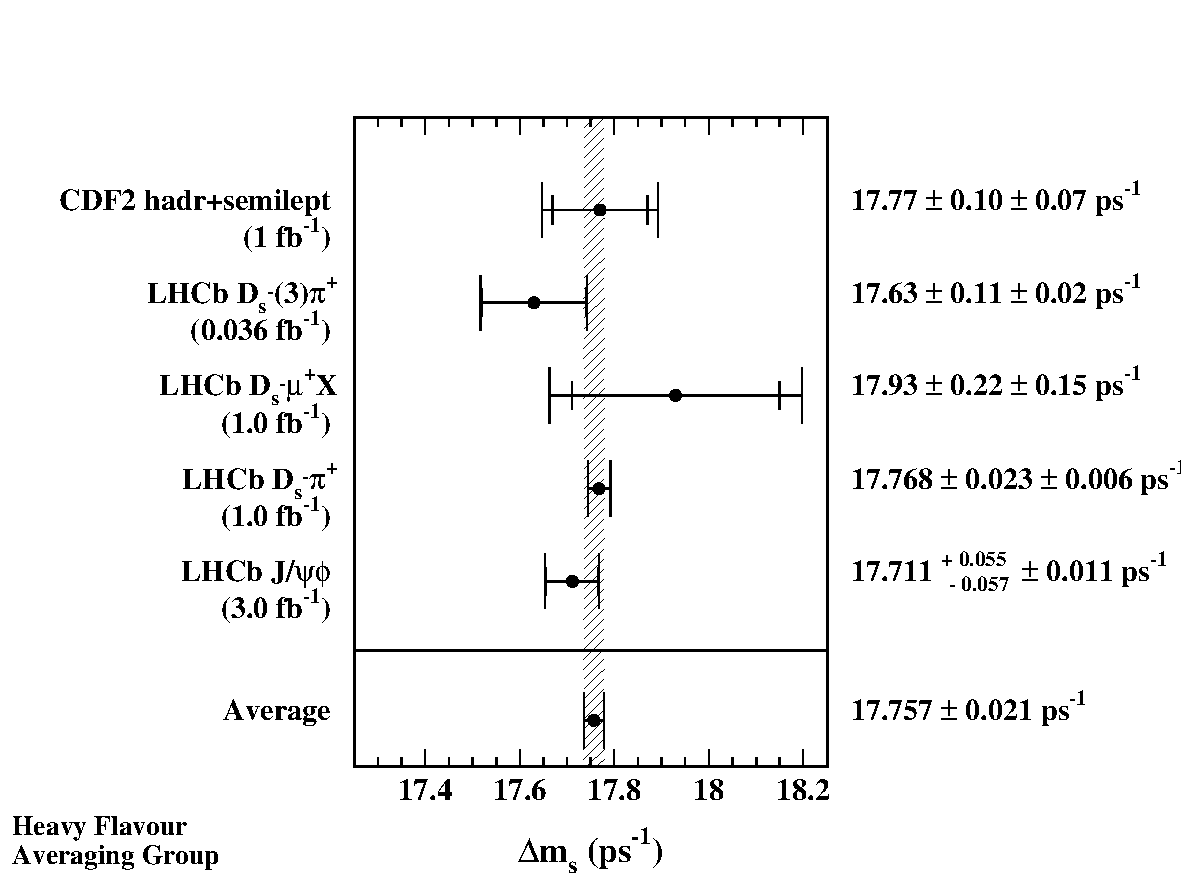
\includegraphics[width=0.8\textwidth]{figures/life_mix/dms_W_bw}
\caption{Published % and recent preliminary
measurements of \dms, together with their average.} 
\labf{dms}
\end{center}
\end{figure}

A simple average of the CDF and LHCb results\footnote{
  \label{foot:life_mix:D0note5618:2008}
  We do not include the old unpublished
  \dzero~\cite{D0note5618:2008,*D0note5474:2007,*D0note5254:2006,*Abazov:2006dm_mod_cont}
  result in the average.},
taking into account the correlated systematic uncertainties between the three 
LHCb measurements, yields 
\begin{equation}
\dms = \hfagDMSfull = \hfagDMS \labe{dms}
\end{equation}
and is illustrated in \Figure{dms}.
Multiplying this result with the 
mean \Bs lifetime of \Eq{oneoverGs}, $1/\Gs=\hfagTAUBSMEANCON$,
yields
\begin{equation}
\xs = \frac{\dms}{\Gs} = \hfagXS \,. \labe{xs}
\end{equation}
With $2\ys = \DGGs=\hfagDGSGSCON$ 
%(see \Eqss{DGGs_ave}{corrDGGs})
%(see \Eq{DGGs_ave})
(see \Eq{DGs_DGsGs})
and under the assumption of no \CP violation in \Bs mixing,
this corresponds to
\begin{equation}
\chis = \frac{\xs^2+\ys^2}{2(\xs^2+1)} = \hfagCHIS \,. \labe{chis}
\end{equation}
The ratio of the \Bd and \Bs oscillation frequencies, 
obtained from \Eqss{dmd}{dms}, 
\begin{equation}
\frac{\dmd}{\dms} = \hfagRATIODMDDMS \,, \labe{dmd_over_dms}
\end{equation}
can be used to extract the following ratio of CKM matrix elements, 
\begin{equation}
\left|\frac{V_{td}}{V_{ts}}\right| =
\xi \sqrt{\frac{\dmd}{\dms}\frac{m(\Bs)}{m(\Bd)}} = 
\hfagVTDVTSfull \,, \labe{Vtd_over_Vts}
\end{equation}
where the first quoted error is from experimental uncertainties 
(with the masses $m(\Bs)$ and $m(\Bd)$ taken from \Ref{PDG_2012}),
and where the second quoted error is from theoretical uncertainties 
in the estimation of the SU(3) flavour-symmetry breaking factor
$\xi %= (f_{B_s} \sqrt{B_{B_s}})/(f_{B_d} \sqrt{B_{B_d}})
= \hfagXI$
obtained from unquenched lattice QCD calculations~\cite{Aoki:2013ldr_mod}.
%2014% \cite{Laiho:2009eu_mod,*Evans:2008zzg_mod,*Gamiz:2009ku,*Albertus:2010nm}.

%------------------------------------------------
\mysubsubsection{\CP violation in \Bd and \Bs mixing}
%------------------------------------------------
\labs{qpd} \labs{qps}

%---------------------------------------------------------------
% \subsubsubsection{\boldmath \CP violation parameter $|q/p|_{\particle{d}}$}
%---------------------------------------------------------------

Evidence for \CP violation in \Bd mixing
%, which is predicted to be very small in the Standard Model,
has been searched for,
both with flavour-specific and inclusive \Bd decays, 
in samples where the initial 
flavour state is tagged. In the case of semileptonic 
(or other flavour-specific) decays, 
where the final state tag is 
also available, the following asymmetry
\begin{equation} 
\ASLd = \frac{
N(\hbox{\Bdbar}(t) \to \ell^+      \nu_{\ell} X) -
N(\hbox{\Bd}(t)    \to \ell^- \bar{\nu}_{\ell} X) }{
N(\hbox{\Bdbar}(t) \to \ell^+      \nu_{\ell} X) +
N(\hbox{\Bd}(t)    \to \ell^- \bar{\nu}_{\ell} X) } 
= \frac{|p/q|_{\particle{d}}^2 - |q/p|_{\particle{d}}^2}%
{|p/q|_{\particle{d}}^2 + |q/p|_{\particle{d}}^2}
% \simeq 1 - |q/p|^2_{\particle{d}} 
\labe{ASL}
\end{equation} 
has been measured, either in time-integrated analyses at 
CLEO~\cite{Behrens:2000qu,Jaffe:2001hz,*Jaffe:2001hz_cont},
CDF~\cite{Abe:1996zt}% 
\footnote{
  \label{foot:life_mix:CDFnote9015:2007}
  We do not include the unpublished measurement of Ref.~\cite{CDFnote9015:2007} in our average.}
and \dzero~\cite{Abazov:2013uma,*Abazov:2011yk_mod,*Abazov:2010hv_mod_cont,*Abazov:2010hj_mod_cont,*Abazov:2011yk_cont,Abazov:2012uia},
or in time-dependent analyses at 
OPAL~\cite{Ackerstaff:1997vd}, ALEPH~\cite{Barate:2000uk}, 
\babar~\cite{Aubert:2003hd,*Aubert:2004xga_mod_cont,Aubert:2006nf,*Aubert:2002mn_mod_cont,Lees:2013sua,*Margoni:2013qx,*Aubert:2006sa_mod}
and \belle~\cite{Nakano:2005jb}.
In the inclusive case, also investigated and published
% at LEP~\cite{DELPHIconf:1997,Barate:2000uk,Abbiendi:1998av},
at ALEPH~\cite{Barate:2000uk} and OPAL~\cite{Abbiendi:1998av},
no final state tag is used, and the asymmetry~\cite{Beneke:1996hv,*Dunietz:1998av}
\begin{equation} 
\frac{
N(\hbox{\Bd}(t) \to {\rm all}) -
N(\hbox{\Bdbar}(t) \to {\rm all}) }{
N(\hbox{\Bd}(t) \to {\rm all}) +
N(\hbox{\Bdbar}(t) \to {\rm all}) } 
\simeq
\ASLd \left[ \frac{\dmd}{2\Gd} \sin(\dmd \,t) - 
\sin^2\left(\frac{\dmd \,t}{2}\right)\right] 
\labe{ASLincl}
\end{equation} 
must be measured as a function of the proper time to extract information 
on \CP violation.

On the other hand, LHCb has studied the time-dependence of the 
charge asymmetry of $B^0 \to D^{(*)-}\mu^+\nu_{\mu}X$ decays
without tagging the initial state~\cite{Aaij:2014nxa}, 
which would be equal to 
\begin{equation} 
\frac{N(D^{(*)-}\mu^+\nu_{\mu}X)-N(D^{(*)+}\mu^-\bar{\nu}_{\mu}X)}%
{N(D^{(*)-}\mu^+\nu_{\mu}X)+N(D^{(*)+}\mu^-\bar{\nu}_{\mu}X)} =
\ASLd \left[ 1- \cos(\dmd \,t)\right]
\label{eq:untagged_ASL}
\end{equation}
in absence of detection and production asymmetries.

\Table{qoverp} summarized the different measurements: 
in all cases asymmetries compatible with zero have been found,  
with a precision limited by the available statistics. 

\begin{table}
\caption{Measurements\footref{foot:life_mix:Abe:1996zt}
%\addtocounter{footnote}{0}\protect\footnotemark\addtocounter{footnote}{-1}
of \CP violation in \Bd mixing and their average
in terms of both \ASLd and $|q/p|_{\particle{d}}$.
The individual results are listed as quoted in the original publications, 
or converted\footref{foot:life_mix:epsilon_B}
%\addtocounter{footnote}{4}\protect\footnotemark\addtocounter{footnote}{-5}
to an \ASLd value.
% (except in the case of CDF2, where 
% the quoted value of \ASLd has been derived from the original measurement 
% assuming that $\ASLs = 0$). 
When two errors are quoted, the first one is statistical and the 
second one systematic. The ALEPH and OPAL % and CDF2
results assume no \CP violation in \Bs mixing.}
% \ie\ $|q/p|_{\particle{s}}=1$.}
\labt{qoverp}
\begin{center}
\begin{tabular}{@{}rcl@{$\,\pm$}l@{$\pm$}ll@{$\,\pm$}l@{$\pm$}l@{}}
\hline
%Experiment & {Method} & \multicolumn{3}{c}{\ASLd} 
%                      & \multicolumn{3}{c}{$|q/p|_{\particle{d}}$} \\
%Exp.\ \& Ref. & Method & ~~~\ASLd & stat & syst
%                       & $|q/p|_{\particle{d}}$ & stat & syst \\
Exp.\ \& Ref. & Method & \multicolumn{3}{c}{Measured \ASLd} 
                       & \multicolumn{3}{c}{Measured $|q/p|_{\particle{d}}$} \\
\hline
% CLEO   \cite{Behrens:2000qu} & $D^{*\pm}\pi^{\mp}$, $D^{*\pm}\rho^{\mp}$ (part.\ rec.) 
CLEO   \cite{Behrens:2000qu} & partial hadronic rec. 
                             & $+0.017$ & 0.070 & 0.014 
                             & \multicolumn{3}{c}{} \\
CLEO   \cite{Jaffe:2001hz,*Jaffe:2001hz_cont}   & dileptons 
                             & $+0.013$ & 0.050 & 0.005 
                             & \multicolumn{3}{c}{} \\
CLEO   \cite{Jaffe:2001hz,*Jaffe:2001hz_cont}   & average of above two 
                             & $+0.014$ & 0.041 & 0.006 
                             & \multicolumn{3}{c}{} \\
% \babar \cite{Aubert:2002mn}  & dileptons                 % superseded by \cite{Aubert:2006nf,*Aubert:2002mn_mod_cont}
%                              & $+0.005$ & 0.012 & 0.014  % superseded by \cite{Aubert:2006nf,*Aubert:2002mn_mod_cont}
%                              & 0.998 & 0.006 & 0.007 \\  % superseded by \cite{Aubert:2006nf,*Aubert:2002mn_mod_cont}
\babar \cite{Aubert:2003hd,*Aubert:2004xga_mod_cont}   & full hadronic rec. 
                             & \multicolumn{3}{c}{}  
                             & 1.029 & 0.013 & 0.011  \\
\babar \cite{Aubert:2006nf,*Aubert:2002mn_mod_cont}  & dileptons
                             & \multicolumn{3}{c}{}
                             & 0.9992 & 0.0027 & 0.0019 \\ 
\babar \cite{Lees:2013sua,*Margoni:2013qx,*Aubert:2006sa_mod} & part.\ rec.\ $D^{*}X\ell\nu$ 
                             & $+0.0006$ & \multicolumn{2}{@{}l}{$0.0017 ^{+0.0038}_{-0.0032}$} 
                             & $0.99971$ & $0.00084$ & $0.00175$ \\ 
\belle \cite{Nakano:2005jb}  & dileptons 
                             & $-0.0011$ & 0.0079 & 0.0085 
                             & 1.0005 & 0.0040 & 0.0043 \\
%\hline
\multicolumn{2}{l}{Average of above 6 \B factory results} & \multicolumn{3}{l}{\hfagASLDB\ (tot)} 
                             & \multicolumn{3}{l}{\hfagQPDB\  (tot)} \\ 
\hline
\dzero \cite{Abazov:2012uia} & $B^0 \to D^{(*)-}\mu+X$
                            & $+0.0068$ & 0.0045 & 0.0014 & \multicolumn{3}{c}{} \\
LHCb \cite{Aaij:2014nxa} & $B^0 \to D^{(*)-}\mu+X$
                            & $-0.0002$ & 0.0019 & 0.0030 & \multicolumn{3}{c}{} \\
\multicolumn{2}{l}{Average of above 8 pure $B^0$ results} & \multicolumn{3}{l}{\hfagASLDD\ (tot)}
                             & \multicolumn{3}{l}{\hfagQPDD\  (tot)} \\
\hline
\dzero  \cite{Abazov:2013uma,*Abazov:2011yk_mod,*Abazov:2010hv_mod_cont,*Abazov:2010hj_mod_cont,*Abazov:2011yk_cont}  & dimuons  
                             & $-0.0062$ & \multicolumn{2}{@{\hspace{0.26em}}l}{0.0043 (tot)}
                             & \multicolumn{3}{c}{} \\
%\hline
\multicolumn{2}{l}{Average of above 9 direct measurements} & \multicolumn{3}{l}{\hfagASLDW\ (tot)} 
                             & \multicolumn{3}{l}{\hfagQPDW\  (tot)} \\ 
\hline
OPAL   \cite{Ackerstaff:1997vd}   & leptons     
                             & $+0.008$ & 0.028 & 0.012 
                             & \multicolumn{3}{c}{} \\
OPAL   \cite{Abbiendi:1998av}   & inclusive (\Eq{ASLincl}) 
                             & $+0.005$ & 0.055 & 0.013 
                             & \multicolumn{3}{c}{} \\
ALEPH  \cite{Barate:2000uk}       & leptons 
                             & $-0.037$ & 0.032 & 0.007 
                             & \multicolumn{3}{c}{} \\
ALEPH  \cite{Barate:2000uk}       & inclusive (\Eq{ASLincl}) 
                             & $+0.016$ & 0.034 & 0.009 
                             & \multicolumn{3}{c}{} \\
ALEPH  \cite{Barate:2000uk}       & average of above two 
                             & $-0.013$ & \multicolumn{2}{@{\hspace{0.26em}}l}{0.026 (tot)} 
                             & \multicolumn{3}{c}{} \\
%CDF2    \cite{CDFnote9015:2007}$^p$ & dimuons  
%                             & $+0.0136$ & 0.0151 & 0.0115
%                             & \multicolumn{3}{c}{} \\
\multicolumn{2}{l}{Average of above 14 results} & \multicolumn{3}{l}{\hfagASLDA\ (tot)} 
                             & \multicolumn{3}{l}{\hfagQPDA\  (tot)} \\ 
\hline
\multicolumn{5}{l}{Best fit value from 2D combination of} \\
\multicolumn{2}{l}{\ASLd and \ASLs results (see \Eq{ASLD})} & \multicolumn{3}{l}{\hfagASLD\ (tot)} 
                             & \multicolumn{3}{l}{\hfagQPD\  (tot)} \\ 
\hline
% \multicolumn{8}{l}{$^p$ {\footnotesize Preliminary.}}
\end{tabular}
\end{center}
\end{table}

A simple average of all measurements performed at 
%pre-2012% \B factories~\cite{Behrens:2000qu,Jaffe:2001hz,*Jaffe:2001hz_cont,Aubert:2003hd,*Aubert:2004xga_mod_cont,Aubert:2006nf,*Aubert:2002mn_mod_cont,Aubert:2006sa,Nakano:2005jb}
\B factories~\cite{Behrens:2000qu,Jaffe:2001hz,*Jaffe:2001hz_cont,Aubert:2003hd,*Aubert:2004xga_mod_cont,Aubert:2006nf,*Aubert:2002mn_mod_cont,Lees:2013sua,*Margoni:2013qx,*Aubert:2006sa_mod,Nakano:2005jb}
yields $\ASLd = \hfagASLDB$; adding also the \dzero~\cite{Abazov:2012uia}
and LHCb~\cite{Aaij:2014nxa} measurements obtained with reconstructed 
semileptonic \Bd decays yields
\begin{equation}
\ASLd = \hfagASLDD  ~~~ \Longleftrightarrow ~~~ |q/p|_{\particle{d}} = \hfagQPDD \,,
\labe{ASLDD}
\end{equation}
where the relation between \ASLd and $|q/p|_{\particle{d}}$ is given in \Eq{ASL}.
The latest dimuon \dzero analysis~\cite{Abazov:2013uma,*Abazov:2011yk_mod,*Abazov:2010hv_mod_cont,*Abazov:2010hj_mod_cont,*Abazov:2011yk_cont}
separates the \Bd and \Bs contributions by exploiting the dependence on the muon impact parameter cut; combining the 
\ASLd result quoted by \dzero with the above \Bd average of \Eq{ASLDD} yields
%%% \begin{equation}
%%%\ASLd = \hfagASLDW ~~~ \Longleftrightarrow ~~~ |q/p|_{\particle{d}} = \hfagQPDW \,.
%%% \labe{ASLDW}
%%% \end{equation}
$\ASLd = \hfagASLDW$. % and $|q/p|_{\particle{d}} = \hfagQPDW$.

All the other \Bd analyses performed at high energy, either at LEP or at the Tevatron,
did not separate the contributions from the \Bd and \Bs mesons.
Under the assumption of no \CP violation in \Bs mixing, a number of 
these analyses~\cite{Abazov:2006qw,Ackerstaff:1997vd,Barate:2000uk,Abbiendi:1998av}
quote a measurement of $\ASLd$ or $|q/p|_{\particle{d}}$ for the \Bd meson. Including also 
these results%
\footnote{
  \label{foot:life_mix:Abe:1996zt}
  A low-statistics result published by CDF using the Run I data~\cite{Abe:1996zt} and 
an unpublished result by CDF using Run II data~\cite{CDFnote9015:2007} 
are not included in our averages, nor in \Table{qoverp}.}
in the previous average % with the average of \Eq{ASLDW}
leads to 
$\ASLd = \hfagASLDA$ % and $|q/p|_{\particle{d}} = \hfagQPDA$
under the assumption $\ASLs =0$. The latter assumption makes sense within the Standard Model, 
since \ASLs is predicted to be much smaller than \ASLd~\cite{Lenz:2011ti,*Lenz:2006hd}, but may not be suitable
in presence of New Physics. 

%---------------------------------------------------------------
% \subsubsubsection{\boldmath \CP violation parameter $|q/p|_{\particle{s}}$}
%---------------------------------------------------------------

The following constraints on a combination of \ASLd and \ASLs
(or equivalently $|q/p|_{\particle{d}}$ and $|q/p|_{\particle{s}}$)
have been obtained by the Tevatron 
experiments, using inclusive semileptonic decays of \b hadrons:
\begin{eqnarray}
\frac{1}{4}\left(f'_{\particle{d}} \,\chid \ASLd +
                 f'_{\particle{s}} \,\chis \ASLs \right) &=& 
+0.0015 \pm 0.0038 \mbox{(stat)} \pm 0.0020 \mbox{(syst)}
%f'_{\particle{d}} \,\chid(1-|q/p|^2_{\particle{d}})+
% f'_{\particle{s}} \,\chis(1-|q/p|^2_{\particle{s}}) = +0.006\pm 0.017
~~~ \mbox{CDF1~\cite{Abe:1996zt}} \,, ~
\labe{CDF_ASLDS} \\
% RvK
%\frac{1}{4}\left(\ASLd +
%\ASLs \frac{f'_\particle{s}\chis}{f'_\particle{d}\chid} \right) =
%-0.0023 \pm 0.0011 \mbox{(stat)} \pm 0.0008 \mbox{(syst)}
%&& \mbox{\dzero~\cite{Abazov:2006qw}} \,,
%%2012%%\ASLb = \frac{f'_{\particle{d}}Z_{\particle{d}} \ASLd + f'_{\particle{s}}Z_{\particle{s}} \ASLs}%
%%2012%%{f'_{\particle{d}}Z_{\particle{d}} + f'_{\particle{s}}Z_{\particle{s}}} &=&
%%2012%% -0.00787 \pm 0.00172 \mbox{(stat)} \pm 0.00093 \mbox{(syst)}
%%2012%%~~~ \mbox{\dzero~\cite{Abazov:2011yk_mod,*Abazov:2010hv_mod_cont,*Abazov:2010hj_mod_cont,*Abazov:2011yk_cont}} \,, ~
\ASLb = \frac{f'_{\particle{d}}\chid \ASLd + f'_{\particle{s}}\chis \ASLs}%
{f'_{\particle{d}}\chid + f'_{\particle{s}}\chis} &=&
 -0.00496 \pm 0.00153 \mbox{(stat)} \pm 0.00072 \mbox{(syst)}
~~ \mbox{\dzero~\cite{Abazov:2013uma,*Abazov:2011yk_mod,*Abazov:2010hv_mod_cont,*Abazov:2010hj_mod_cont,*Abazov:2011yk_cont}} \,. ~
\labe{Dzero_ASLDS}
\end{eqnarray}
%%2012%% where\footnote{In \Ref{Abazov:2007zj}, the \dzero result
%%2012%% $\frac{1}{4}\left(\ASLd +
%%2012%% \ASLs \frac{f'_\particle{s}\chis}{f'_\particle{d}\chid} \right) =
%%2012%% -0.0023 \pm 0.0011 \mbox{(stat)} \pm 0.0008 \mbox{(syst)}$~\cite{Abazov:2006qw}
%%2012%% (now superseded by that of \Ref{Abazov:2013uma,*Abazov:2011yk_mod,*Abazov:2010hv_mod_cont,*Abazov:2010hj_mod_cont,*Abazov:2011yk_cont})
%%2012%% was reinterpreted by replacing $\chi_{\particle{s}}/\chi_{\particle{d}}$
%%2012%% with $Z_{\particle{s}}/Z_{\particle{d}}$.
%%2012%% For simplicity, and since this has anyway a negligible numerical effect on our
%%2012%% combined result of \Fig{ASLs}, % \Eq{ASLSW},
%%2012%% we follow the same interpretation and set
%%2012%% $\chi_{\particle{q}}=Z_{\particle{q}}/2$ in \Eq{CDF_ASLDS}.
%%2012%% We also set $f'_{\particle{q}}=f_{\particle{q}}$.}
%%2012%% $Z_{\particle{q}} = 1/(1-y_{\particle{q}}^2)-1/(1+x_{\particle{q}}^2)
%%2012%% = 2 \chi_{\particle{q}}/(1-y_{\particle{q}}^2)$, $q=d,s$.
While the imprecise CDF1 result is compatible with no \CP violation%
\footnote{
  \label{foot:life_mix:CDFnote9015:2007-2}
  A measurement from CDF2, 
$ \ASLb = +0.0080 \pm 0.0090 \mbox{(stat)} \pm 0.0068 \mbox{(syst)}$~\cite{CDFnote9015:2007},
more precise than the \dzero measurement,
is also compatible with no \CP violation,
but since it is unpublished since 2007 
we no longer include it in our averages, nor in \Fig{ASLs}.},
the \dzero result of \Eq{Dzero_ASLDS}, obtained by measuring
the charge asymmetry of like-sign dimuons, differs by 2.8 standard
deviations from the Standard Model expectation of
%\begin{eqnarray}
%\mbox{\hspace{3cm}}
$\ASLb({\mathrm{SM}}) = (-2.3\pm 0.4) \times 10^{-4}$%
~\cite{Abazov:2013uma,*Abazov:2011yk_mod,*Abazov:2010hv_mod_cont,*Abazov:2010hj_mod_cont,*Abazov:2011yk_cont,Lenz:2011ti,*Lenz:2006hd}.
%&~~& \mbox{\cite{Abazov:2013uma,*Abazov:2011yk_mod,*Abazov:2010hv_mod_cont,*Abazov:2010hj_mod_cont,*Abazov:2011yk_cont,Lenz:2011ti,*Lenz:2006hd}}\,.
%\end{eqnarray}
With a more sophisticated analysis in bins of the
muon impact parameters, \dzero conclude that the overall deviation of the 
their measurements from the SM is at the level of $3.6\,\sigma$.

Using the average $\ASLd = \hfagASLDD$ of \Eq{ASLDD},
obtained from pure \Bd measurements,
%%2012%% the averages 
%%2012%% of the Tevatron $b$-hadron fractions and their correlations listed in \Table{fractions},
%%2012%% and the averages of the mixing parameters 
%%2012%% presented in this chapter,
the two results of \Eqss{CDF_ASLDS}{Dzero_ASLDS}
are turned\footnote{
  \label{foot:life_mix:f'f}
  For simplicity, we set $f'_{\particle{q}}=f_{\particle{q}}$.} 
into the measurements of \ASLs displayed in the top part of \Fig{ASLs}.
\begin{figure}[t]
\begin{center}
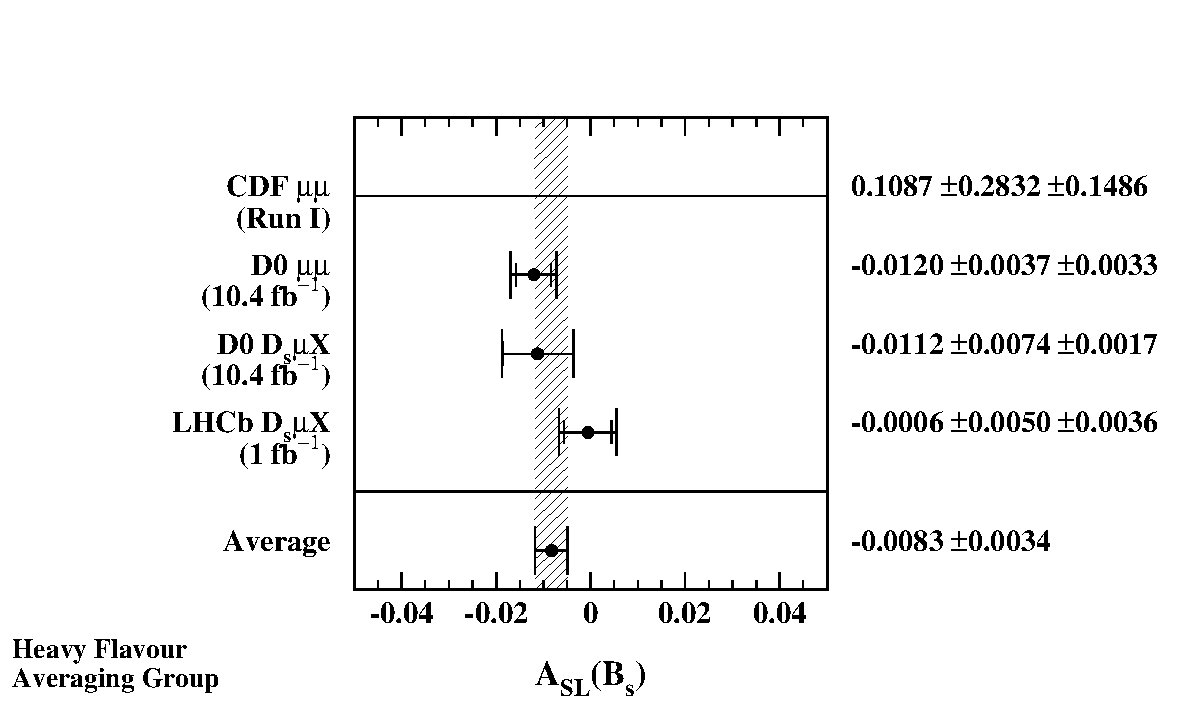
\includegraphics[width=0.8\textwidth]{figures/life_mix/asls_bw}
\caption{Measurements of \ASLs,
derived from CDF~\cite{Abe:1996zt},\footref{foot:life_mix:CDFnote9015:2007-2}
%\addtocounter{footnote}{-2}\protect\footnotemark\addtocounter{footnote}{1},
\dzero~\cite{Abazov:2013uma,*Abazov:2011yk_mod,*Abazov:2010hv_mod_cont,*Abazov:2010hj_mod_cont,*Abazov:2011yk_cont,Abazov:2012zz,*Abazov:2009wg_mod_cont,*Abazov:2007nw_mod_cont}
and LHCb~\cite{Aaij:2013gta}
analyses, adjusted to the pure \Bd 
average of \ASLd. 
%%2012%%, the Tevatron averages of the \b-hadron fractions, and the latest averages of the mixing parameters. 
The combined value of \ASLs is also shown.}
\labf{ASLs}
\end{center}
\end{figure}
Taking into account the uncertainties on
%%2012%% $f'_{\particle{d}}, f'_{\particle{s}}, Z_{\particle{d}},$ and $Z_{\particle{s}}$,
the \b-hadron fractions and mixing parameters, 
the value derived from the \dzero analysis does not show evidence
of \CP violation in the \Bs system.
In addition, the third and fourth lines of \Fig{ASLs} show direct determination of \ASLs
% and hence $|q/p|_{\particle{s}}$ 
obtained by \dzero~\cite{Abazov:2012zz,*Abazov:2009wg_mod_cont,*Abazov:2007nw_mod_cont}
and LHCb~\cite{Aaij:2013gta}
by measuring the time-integrated charge asymmetry of
untagged $\Bs \to D_s \mu X$ decays.
The four results of \Fig{ASLs} are
combined to yield
%%% \begin{equation}
%%% \ASLs = \hfagASLSWval\hfagASLSWsta\mbox{(stat)}\hfagASLSWsys\mbox{(syst)} = \hfagASLSW
%%% \labe{ASLSW}
%%% \end{equation}
$\ASLs = \hfagASLSWval\hfagASLSWsta\mbox{(stat)}\hfagASLSWsys\mbox{(syst)} = \hfagASLSW$
or, equivalently through \Eq{ASL},
%%% \begin{equation}
%%% |q/p|_{\particle{s}} = \hfagQPSWval\hfagQPSWsta\mbox{(stat)}\hfagQPSWsys\mbox{(syst)} = \hfagQPSW \,.
%%% \labe{QPSW}
%%% \end{equation}
$|q/p|_{\particle{s}} = \hfagQPSWval\hfagQPSWsta\mbox{(stat)}\hfagQPSWsys\mbox{(syst)} = \hfagQPSW$.
The quoted systematic errors include experimental systematics as well as the correlated dependence on external 
parameters. 
%%% These results are compatible with no \CP violation in \Bs mixing.

As mentioned above, the \dzero like-sign dimuon analysis investigates 
the dependence of the charge asymmetry 
as a function of the muon impact parameters. 
%%2012%%, allowing the separation of the 
%%2012%%\Bd and \Bs contributions to the result of \Eq{Dzero_ASLDS}.
Interpreting the observed asymmetries in terms of \CP violation in $B$ meson mixing and interference, 
and using 
the mixing parameters and the world $b$-hadron fractions 
of \Ref{Amhis:2012bh}, the \dzero collaboration
extracts~\cite{Abazov:2013uma,*Abazov:2011yk_mod,*Abazov:2010hv_mod_cont,*Abazov:2010hj_mod_cont,*Abazov:2011yk_cont}
values for \ASLd and \ASLs and their correlation
coefficient\footnote{
  \label{foot:life_mix:Abazov:2013uma}
  They also extract at the same time a value for \DGGd (see \Sec{DGd}).}, 
as shown in the first line of \Table{ASLs_ASLd}.
However, the individual 
contributions to the total quoted errors from this analysis and from the
external inputs are not given, so the adjustment of these results to different
or more recent values of the external inputs cannot (easily) be done. 
Using a two-dimensional fit, these values are combined with the pure
\Bd average of \Eq{ASLDD} and with the results from the 
$\Bs \to D_s \mu X$ analyses~\cite{Abazov:2012zz,*Abazov:2009wg_mod_cont,*Abazov:2007nw_mod_cont,Aaij:2013gta},
assumed to be independent and also shown in \Table{ASLs_ASLd}.
The result, shown graphically in \Fig{ASLs_ASLd}, is 
\begin{table}
\caption{Direct measurements of \CP violation in \Bs and \Bd mixing, together 
with their two-dimensional average. Only total errors are quoted.}
\labt{ASLs_ASLd}
\begin{center}
\begin{tabular}{ccccc}
\hline
Exp.\ \& Ref.\ & Method & Measured \ASLs & Measured \ASLd & $\rho(\ASLs,\ASLd)$ \\
\hline
\dzero  \cite{Abazov:2012zz,*Abazov:2009wg_mod_cont,*Abazov:2007nw_mod_cont}  & $\Bs \to D_s \mu X$ 
       & $-0.0112 \pm 0.0076$ % ASLs = -0.0112 +-0.0074(stat) +0.0017(syst)
       & & \\
LHCb \cite{Aaij:2013gta} & $\Bs \to D_s \mu X$ & $-0.0006 \pm 0.0062$ & & \\
\hline
\multicolumn{2}{l}{Average of above \Bs results}
       & \hfagASLSD & & \\ 
\multicolumn{2}{l}{Average of \Bd results (\Eq{ASLDD})} 
       & & \hfagASLDD & \\ 
\dzero  \cite{Abazov:2013uma,*Abazov:2011yk_mod,*Abazov:2010hv_mod_cont,*Abazov:2010hj_mod_cont,*Abazov:2011yk_cont}  & dimuons  
       & $-0.0082 \pm 0.0099$ % ASLs
       & $-0.0062 \pm 0.0043$ % ASLd
       & $-0.61$ \\          % rho
\hline
\multicolumn{2}{l}{Average of all above}
       & \hfagASLS & \hfagASLD & $\hfagRHOASLSASLD$ \\ 
\hline
%\multicolumn{5}{l}{$^p$ {\footnotesize Preliminary.}}
\end{tabular}
\end{center}
\end{table}
\begin{figure}
\begin{center}
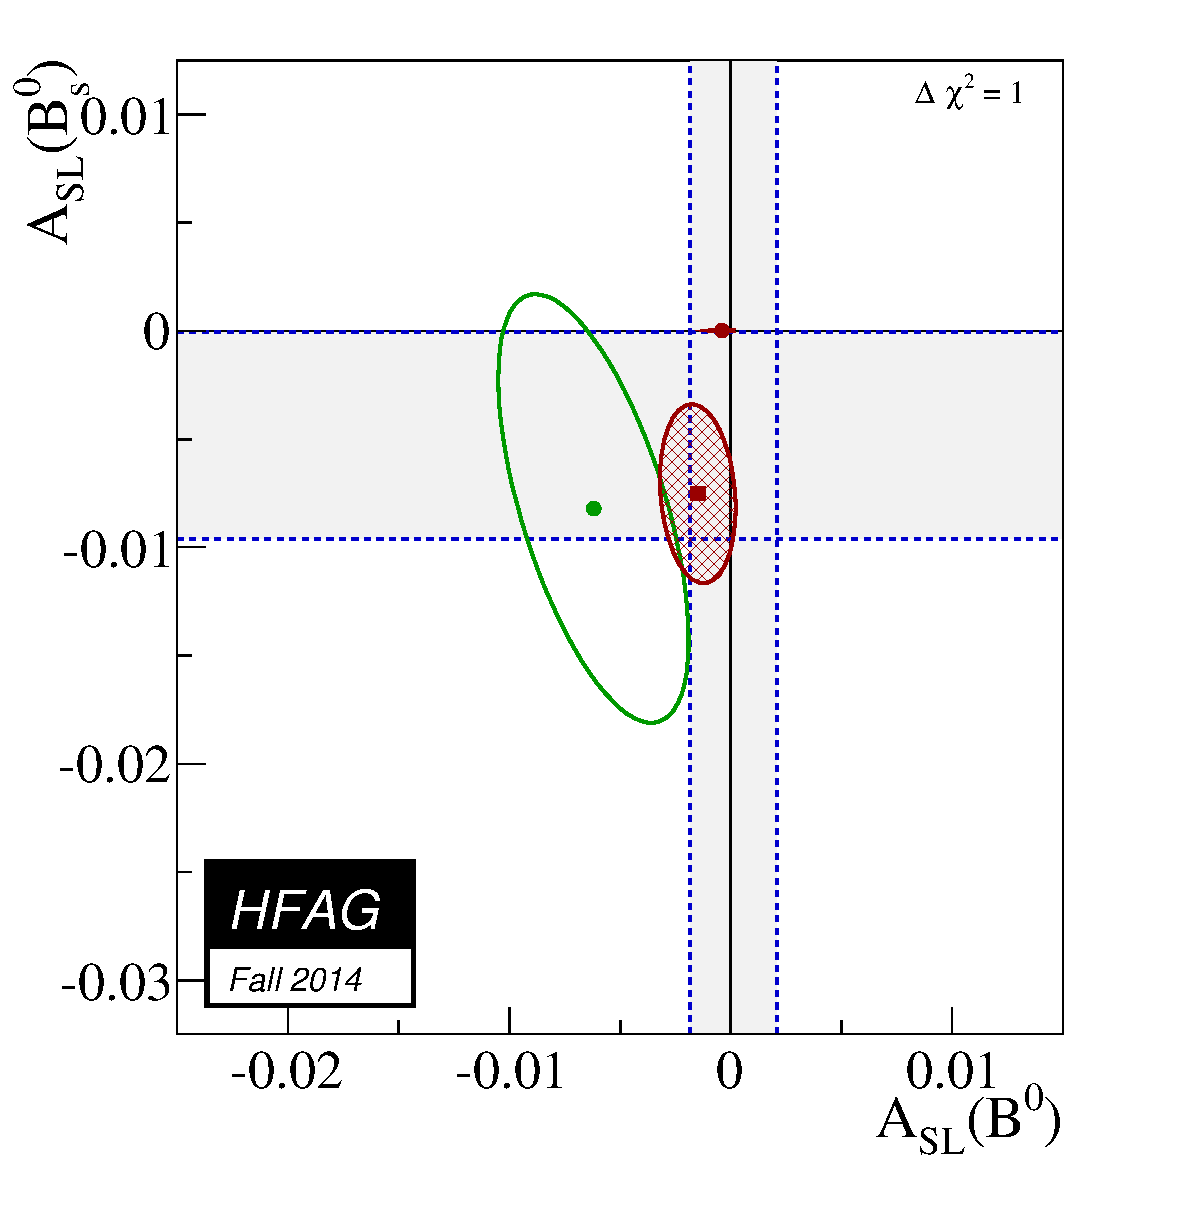
\includegraphics[width=0.6\textwidth]{figures/life_mix/asls_asld}
\end{center}
\vspace{-5mm}
\caption{
Direct measurements of \ASLs and \ASLd listed in \Table{ASLs_ASLd}
(\Bd average as the vertical band, \Bs average as the horizontal band,
\dzero dimuon result as the green ellipse),
together with their two-dimensional average (red hatched ellipse).
%%% Direct measurements of \ASLs and \ASLd listed in \Table{ASLs_ASLd}
%%% (\B-factory average as the vertical blue dotted band, \dzero measurements as the horizontal green dotted band and as the 
%%% green ellipse), together with their two-dimensional average (red hatched ellipse). 
The red point close to $(0,0)$ is the Standard Model prediction
of \Ref{Lenz:2011ti,*Lenz:2006hd} with error bars multiplied by 10.
The prediction and the experimental average deviate from each other by $\hfagASLDASLSNSIGMA\,\sigma$.}
\labf{ASLs_ASLd}
\end{figure}
\begin{eqnarray}
\ASLd & = & \hfagASLD ~~~ \Longleftrightarrow ~~~ |q/p|_{\particle{d}} = \hfagQPD \,,
\labe{ASLD}
\\
\ASLs & = & \hfagASLS ~~~ \Longleftrightarrow ~~~ |q/p|_{\particle{s}} = \hfagQPS \,,
\labe{ASLS}
\\
\rho(\ASLd , \ASLs) & = & \hfagRHOASLSASLD \,.
\labe{rhoASLDASLS}
\end{eqnarray}
%%% and has a correlation of \hfagRHOASLSASLD with the \ASLd value already quoted in \Eq{ASLD}.

The average of \Fig{ASLs} % \Eq{ASLSW}
ignores the impact parameter study of \dzero.
%%2012%% and is adjusted to the $b$-hadron fractions at the Tevatron.
The average of \Eq{ASLS} ignores the CDF1 
result, which has a very large uncertainty anyway.
%%2012%% and is adjusted to the $b$-hadron fractions at LEP.
%They have almost the same total uncertainty and are equally valid.
We choose the results of \Eqsss{ASLD}{ASLS}{rhoASLDASLS}
as our final averages\footnote{
  \label{foot:life_mix:epsilon_B}
  Early analyses and (perhaps hence) the PDG use the complex
  parameter $\epsilon_{\B} = (p-q)/(p+q)$; if \CP violation in the mixing in small,
  $\ASLd \cong 4 {\rm Re}(\epsilon_{\B})/(1+|\epsilon_{\B}|^2)$ and the averages of
  \Eqss{ASLDD}{ASLD} % \Eqsss{ASLDD}{ASLDW}{ASLD}
  correspond to ${\rm Re}(\epsilon_{\B})/(1+|\epsilon_{\B}|^2)=\hfagREBDD$ %, $\hfagREBDW$
  and $\hfagREBD$, respectively.},
since they better incorporate the available published data. 

The above averages show no evidence of \CP violation in \Bd and \Bs mixing.
They deviate by $\hfagASLDASLSNSIGMA\,\sigma$ from the very small predictions of the Standard Model, 
${\ASLd}^{\rm SM} = -(4.1\pm 0.6)\times 10^{-4}$ and 
${\ASLs}^{\rm SM} = +(1.9\pm 0.3)\times 10^{-5}$~\cite{Lenz:2011ti,*Lenz:2006hd}.
Given the current size of the experimental uncertainties, there is still 
significant room for
a possible New Physics contribution, especially in the \Bs system. 
In this respect, the deviation of the \dzero dimuon
asymmetry~\cite{Abazov:2013uma,*Abazov:2011yk_mod,*Abazov:2010hv_mod_cont,*Abazov:2010hj_mod_cont,*Abazov:2011yk_cont}
from expectation has generated a lot of excitement, however recent results from D0 and LHCb 
have not yet settled the issue, and more experimental data (especially from LHCb) is awaited eagerly. 

At the more fundamental level, \CP violation in \Bs
mixing\footnote{
  \label{foot:life_mix:CPVinBd}
  Of course, a similar formalism exists for the \Bd system; for 
  simplicity we omit here the subscript $s$ for $\phi_{12}$, $M_{12}$ and $\Gamma_{12}$.}
is caused by the weak phase difference 
% Let us define the \CP-violating weak phase difference
\begin{equation}
\phi_{12} = \arg \left[ -{M_{12}}/{\Gamma_{12}} \right], 
\end{equation}
where $M_{12}$ and $\Gamma_{12}$ are the off-diagonal
elements of the mass and decay matrices of the $\Bs-\Bsbar$ system.
This is related to the observed decay-width difference through the relation
\begin{equation}
\DGs = 2|\Gamma_{12}|\cos\phi_{12}+
{\cal O} \left( \left|\frac{\Gamma_{12}}{M_{12}}\right|^2 \right) \,,
\end{equation}
where quadratic (or higher-order) terms in the small quantity
$|\Gamma_{12}/M_{12}| \sim {\cal O}(m_b^2/m_t^2)$ can be neglected. 
The SM prediction for this phase is tiny~\cite{Lenz:2011ti,*Lenz:2006hd},
\begin{equation}
% \phi_{12}^{\rm SM} = 0.0038\pm0.0010 \,;
\phi_{12}^{\rm SM} = \hfagPHISTWELVESM \,;
\labe{phis12SM}
\end{equation}
however, new physics in \Bs mixing could change this observed phase to
\begin{equation}
\phi_{12} = \phi_{12}^{\rm SM} + \phi_{12}^{\rm NP} \,.
\labe{phi12NP}
\end{equation}
The \Bs semileptonic asymmetry can be expressed as~\cite{Beneke:2003az}
\begin{equation}
\ASLs = 
\Im \left(\frac{\Gamma_{12}}{M_{12}} \right) +
{\cal O} \left( \left|\frac{\Gamma_{12}}{M_{12}}\right|^2 \right) =
\frac{\DGs}{\dms}\tan\phi_{12} +
{\cal O} \left( \left|\frac{\Gamma_{12}}{M_{12}}\right|^2 \right) \,.
\labe{ASLS_tanphi12}
\end{equation}
Using this relation, the current knowledge of \ASLs, \DGs and \dms, 
given in \Eqsss{ASLS}{DGs_DGsGs}{dms} respectively, yield an
experimental determination of $ \phi_{12}$,
\begin{equation}
\tan\phi_{12} = \ASLs \frac{\dms}{\DGs} = \hfagTANPHI \,,
\labe{tanphi12}
\comment{ % start python
from math import *
asls = -0.010460 ; easls = 0.006400
dms = 17.719032  ; edms = 0.042701
dgs = 0.0951919  ; edgs = 0.01362480381803716 
tanphi12 = asls*dms/dgs
etanphi12 = tanphi12*sqrt((easls/asls)**2+(edms/dms)**2+(edgs/dgs)**2)
print tanphi12, etanphi12
} % end python
\end{equation}
which only represents a very weak constraint at present.

%%% In order to better exploit the available data, a two-dimensional fit of all
%%% direct measurements of \ASLd and \ASLs can be performed. This fit, described 
%%% in \Sec{qps} and shown in \Fig{ASLs_ASLd}, gives 
%%% \begin{equation}
%%% \ASLd = \hfagASLD ~~~ \Longleftrightarrow ~~~ |q/p|_{\particle{d}} = \hfagQPD \,,
%%% \labe{ASLD}
%%% \end{equation}
%%% which we take as our final average for \ASLd and $|q/p|_{\particle{d}}$.
%%% All these results\footnote{Early analyses and (perhaps hence) the PDG use the complex
%%% parameter $\epsilon_{\B} = (p-q)/(p+q)$; if \CP violation in the mixing in small, 
%%% $\ASLd \cong 4 {\rm Re}(\epsilon_{\B})/(1+|\epsilon_{\B}|^2)$ and the averages of 
%%% \Eqss{ASLDD}{ASLD} % \Eqsss{ASLDD}{ASLDW}{ASLD}
%%% correspond to ${\rm Re}(\epsilon_{\B})/(1+|\epsilon_{\B}|^2)=\hfagREBDD$ %, $\hfagREBDW$
%%% and $\hfagREBD$, respectively.},
%%% summarized in \Table{qoverp},
%%% are compatible with no \CP violation in \Bd and \Bs mixing. % , an assumption we make for the rest of this section.

%------------------------------------------------
\mysubsubsection{Mixing-induced \CP violation in \Bs decays}
%------------------------------------------------

%%%%%%%%%%%%%%%%%%%%%%%%%%%%%%%%%%%%%%%%%%%%%%%%
%
% This is file life_mix_phis.tex containing
% the subsection about the phi_s
%
%%%%%%%%%%%%%%%%%%%%%%%%%%%%%%%%%%%%%%%%%%%%%%%
%

%---------------------------------------------
% \subsubsubsection{Weak phase in \Bs mixing}
%---------------------------------------------
\labs{phasebs}

%%% \noindent
%%% \fbox{\parbox{\textwidth}{{\bf WARNING}: Several new results became available but are not yet included in the averages, plots, tables and discussion of this paragraph. These include:
%%% \newline$\bullet$ a finalized version of the analysis described in note ATLAS-CONF-2013-039~\cite{Aad:2014cqa,*Aad:2012kba_cont}; 
%%% \newline$\bullet$ a preliminary $\B_s \to\jpsi\phi$ analysis from CMS~\cite{CMS-PAS-BPH-13-012};
%%% \newline$\bullet$ a new $\phi_s$ result with $B^0_s\to\jpsi\pi^+\pi^-$ from LHCb~\cite{Aaij:2014dka,*Aaij:2013oba_supersede};
%%% \newline$\bullet$ a new $\phi_s$ result with $B^0_s\to\jpsi K^+K^-$ from LHCb~\cite{LHCB-PAPER-2014-059,*Aaij:2013oba_supersede2};
%%% \newline$\bullet$ a new $\phi_s$ result with $\bar{B}^0_s\to D_s^+D_s^-$ decays from LHCb~\cite{Aaij:2014ywt}.
%%% \newline These new results have been added to \Table{phisDGsGs}, but otherwise the text has not been updated.
%%% }}
%%% \marginpar{XXX}

\CP violation induced by $\Bs-\Bsbar$ mixing
% in $b \to c\bar{c}s$ decays
has been a field of 
very active study and fast experimental progress 
in the past couple of years.
Similarly to what has happened at the \B factories 
a decade ago, when the \Bd mixing-induced phase $2\beta$
was measured, the Tevatron and LHC experiments are 
now obtaining point estimates
of the \Bs mixing-induced phase \phiccbars.
This \CP-violating phase is defined as 
the weak phase difference between
the $\Bs-\Bsbar$ mixing amplitude
and the $b \to c\bar{c}s$ decay amplitude.

The golden mode for such studies is 
$\Bs \to \jpsi\phi$, followed by $\jpsi \to \mu^+\mu^-$ and 
$\phi\to K^+K^-$, for which a full angular 
analysis of the decay products is performed to 
separate statistically the \CP-even and \CP-odd
contributions in the final state. As already mentioned in 
\Sec{DGs},
CDF~\cite{Aaltonen:2012ie,*CDF:2011af,*Aaltonen:2007he_mod,*Aaltonen:2007gf_mod},
\dzero~\cite{Abazov:2011ry,*Abazov_mod:2008fj,*Abazov:2007tx_mod_cont},
ATLAS~\cite{Aad:2014cqa,*Aad:2012kba_cont}, CMS~\cite{CMS-PAS-BPH-13-012}
and LHCb~\cite{LHCB-PAPER-2014-059,*Aaij:2013oba_supersede2}
have used both untagged and tagged $\Bs \to \jpsi\phi$ (and $\Bs \to \jpsi K^+K^-$) events 
for the measurement of \phiccbars.
LHCb~\cite{Aaij:2014dka,*Aaij:2013oba_supersede}
is using $\Bs \to \jpsi \pi^+\pi^-$ events, 
analyzed with a full amplitude model
including several $\pi^+\pi^-$ resonances (\eg $f_0(980)$),
although the
$\jpsi \pi^+\pi^-$ final state had already been shown
to be almost \CP pure with a \CP-odd fraction
larger than 0.977 at 95\% CL~\cite{LHCb:2012ae}. 
In addition, LHCb is using the $\Bs \to \Ds\Ds$ channel~\cite{Aaij:2014ywt} to measure $\phi_s$.

All CDF, D0, ATLAS and CMS analyses provide 
two mirror solutions related by the transformation 
$(\DGs, \phi_s) \to (-\DGs, \pi-\phi_s)$. However, the
LHCb analysis of $\Bs \to \jpsi K^+K^-$ resolves this ambiguity and 
rules out the solution with negative \DGs~\cite{Aaij:2012eq}.
Therefore, in what follows we only consider the solution with $\DGs > 0$.

%% Text from OL:
%%% The relative phase between the \Bs mixing amplitude and that of
%%% specific $b \to c\bar{c}s$ quark transitions such as 
%%% for \Bs or \Bsbar $\to \jpsi \phi$,
%%% is called \phiccbars. %~\cite{Lenz:2011ti,*Lenz:2006hd,Charles:2011va_mod,*Bona:2006ah}: 

%OLD% \begin{table}
%OLD% \caption{Direct experimental measurements of \phiccbars, \DGs and \Gs using
%OLD% $\Bs\to\jpsi\phi$, $\Bs\to\jpsi K^+K^-$ and $\Bs\to\jpsi\pi^+\pi^-$ decays.
%OLD% Only the solution with $\DGs > 0$ is shown, since the two-fold ambiguity has been
%OLD% resolved in \Ref{Aaij:2012eq}. The first error is due to 
%OLD% statistics, the second one to systematics. The last line gives our average.}
%OLD% \labt{phisDGsGs}
%OLD% \begin{center}
%OLD% \begin{tabular}{@{}l@{\,}l@{\,}l@{\,}|@{\,}l@{\,}|@{\,}l@{\,}|@{\,}l@{}} 
%OLD% \hline
%OLD% Exp.\ & Mode & Ref.\ & \multicolumn{1}{c@{\,}|@{\,}}{\phiccbars}
%OLD%                      & \multicolumn{1}{c@{\,}|@{\,}}{\DGs (\!\!\invps)}
%OLD%                      & \multicolumn{1}{c@{}}{\Gs (\!\!\invps)} \\ 
%OLD% \hline
%OLD% CDF    & $\jpsi\phi$ & \cite{Aaltonen:2012ie,*CDF:2011af,*Aaltonen:2007he_mod,*Aaltonen:2007gf_mod}
%OLD%        & $[-0.60,\, 0.12]$, 68\% CL & $0.068\pm0.026\pm0.009$ % syst error was +-0.007 instead of +-0.009 in CDF note 10778
%OLD%        & $0.654\pm0.008\pm0.004$ \\ % quoted in paper as tau(Bs) = 1/Gamma_s = 1.528 +-0.019 +-0.009
%OLD% % 1./1.528 = 0.6544502617801047, 0.019/1.528**2 = 0.008137797757736905, 0.009//1.528**2 = 0.003854746306296428
%OLD% \dzero & $\jpsi\phi$ & \cite{Abazov:2011ry,*Abazov_mod:2008fj,*Abazov:2007tx_mod_cont}
%OLD%        & $-0.55^{+0.38}_{-0.36}$ & $0.163^{+0.065}_{-0.064}$ & $0.693^{+0.018}_{-0.017}$  \\
%OLD% ATLAS  & $\jpsi\phi$ & \cite{Aad:2014cqa,*Aad:2012kba_cont}
%OLD%        & $+0.12 \pm 0.25 \pm 0.05$ & $0.053 \pm0.021 \pm0.010$ & $0.677 \pm0.007 \pm0.004$ \\
%OLD% %%% CMS    & $\jpsi\phi$ & \cite{CMS-PAS-BPH-11-006}$^p$   % this CMS result not included in the (phi_s, DGs) averaging !
%OLD% %%%        & (set to $0$) & $0.048\pm0.024\pm0.003$ & --- \\
%OLD% CMS    & $\jpsi\phi$ & \cite{CMS-PAS-BPH-13-012}$^p$
%OLD%        & $-0.03 \pm 0.11 \pm 0.03$ & $0.096\pm0.014\pm0.007$ & $0.670 \pm0.004 \pm0.005$ \\
%OLD% %%% the CMS note CMS-PAS-BPH-13-012 quote a "mean Bs lifetime" of
%OLD% %%%    ctau = 447.3 +-3.0 +-3.5 microns = 1.492 +-0.010 +-0.012 ps
%OLD% %%%    corresponding to Gamma_s = 0.6702 +-0.0045 +-0.0052 ps-1
%OLD% LHCb   & $\jpsi KK$ & \cite{LHCB-PAPER-2014-059,*Aaij:2013oba_supersede2}
%OLD%        & $-0.058\pm0.049\pm0.006$ & $0.0805\pm0.0091\pm0.0033$ & $0.6603\pm0.0027\pm0.0015$  \\
%OLD% LHCb   & $\jpsi\pi\pi$ & \cite{Aaij:2014dka,*Aaij:2013oba_supersede}
%OLD%        & $+0.070 \pm0.068 \pm 0.008$ & --- & --- \\
%OLD% LHCb   & $\jpsi hh$ & \cite{LHCB-PAPER-2014-059,*Aaij:2013oba_supersede2}
%OLD%        & $-0.010\pm0.040(\rm tot)$ & --- & --- \\
%OLD% LHCb   & $D_sD_s$ & \cite{Aaij:2014ywt}
%OLD%        & $+0.02 \pm0.17 \pm 0.02$ & --- & --- \\
%OLD% %old%LHCb   & $\jpsi KK$ & \cite{Aaij:2013oba,*LHCb:2011aa_mod,*LHCb:2012ad_mod,*LHCb:2011ab_mod,*Aaij:2012nta_mod}
%OLD% %old%       & $+0.07\pm0.09\pm0.01$ & $0.100\pm0.016\pm0.003$ & $0.663\pm0.005\pm0.006$  \\
%OLD% %old%LHCb   & $\jpsi\pi\pi$ & \cite{Aaij:2013oba,*LHCb:2011aa_mod,*LHCb:2012ad_mod,*LHCb:2011ab_mod,*Aaij:2012nta_mod}
%OLD% %old%       & $-0.014 ^{+0.17}_{-0.16}\pm 0.01$ & --- & --- \\
%OLD% %old%LHCb   & combined & \cite{Aaij:2013oba,*LHCb:2011aa_mod,*LHCb:2012ad_mod,*LHCb:2011ab_mod,*Aaij:2012nta_mod}
%OLD% %old%       & $+0.01\pm0.07\pm0.01$ & $0.106\pm0.011\pm0.007$ & $0.661\pm0.004\pm0.006$  \\
%OLD% \hline
%OLD% \multicolumn{3}{@{}l@{\,}|@{\,}}{All combined} & \hfagPHISCOMB & \hfagDGSCOMBnounit & \hfagGSnounit \\
%OLD% \hline
%OLD% \multicolumn{6}{l}{$^p$ {\footnotesize Preliminary.}}
%OLD% \end{tabular}
%OLD% \end{center}
%OLD% \end{table}

\begin{table}
\caption{Direct experimental measurements of \phiccbars, \DGs and \Gs using
$\Bs\to\jpsi\phi$, $\jpsi K^+K^-$, $\jpsi\pi^+\pi^-$ and $D_s^+D_s^-$ decays.
Only the solution with $\DGs > 0$ is shown, since the two-fold ambiguity has been
resolved in \Ref{Aaij:2012eq}. The first error is due to 
statistics, the second one to systematics. The last line gives our average.}
\labt{phisDGsGs}
\begin{center}
%\begin{tabular}{l@{\,}l@{\,}l@{\,}|@{\,}l@{\,}|@{\,}l@{\,}|@{\,}l} 
\begin{tabular}{llrlll} 
\hline
% Exp.\ & Mode & Dataset & \multicolumn{1}{c@{\,}|@{\,}}{\phiccbars}
%                      & \multicolumn{1}{c@{}}{\DGs (\!\!\invps)} & Ref.\ \\
Exp.\ & Mode & Dataset & \multicolumn{1}{c}{\phiccbars}
                     & \multicolumn{1}{c}{\DGs (\!\!\invps)} & Ref.\ \\
\hline
CDF    & $\jpsi\phi$ & $9.6\invfb$
       & $[-0.60,\, 0.12]$, 68\% CL & $0.068\pm0.026\pm0.009$
       & \cite{Aaltonen:2012ie,*CDF:2011af,*Aaltonen:2007he_mod,*Aaltonen:2007gf_mod} \\
       % syst error was +-0.007 instead of +-0.009 in CDF note 10778
       % & $0.654\pm0.008\pm0.004$ \\ % quoted in paper as tau(Bs) = 1/Gamma_s = 1.528 +-0.019 +-0.009
% 1./1.528 = 0.6544502617801047, 0.019/1.528**2 = 0.008137797757736905, 0.009//1.528**2 = 0.003854746306296428
\dzero & $\jpsi\phi$ & $8.0\invfb$
       & $-0.55^{+0.38}_{-0.36}$ & $0.163^{+0.065}_{-0.064}$ % & $0.693^{+0.018}_{-0.017}$  \\
       & \cite{Abazov:2011ry,*Abazov_mod:2008fj,*Abazov:2007tx_mod_cont} \\
ATLAS  & $\jpsi\phi$ & $4.9\invfb$
       & $+0.12 \pm 0.25 \pm 0.05$ & $0.053 \pm0.021 \pm0.010$ % & $0.677 \pm0.007 \pm0.004$ \\
       & \cite{Aad:2014cqa,*Aad:2012kba_cont} \\
%%% CMS    & $\jpsi\phi$ & $X.X\invfb$ % this CMS result not included in the (phi_s, DGs) averaging !
%%%        & (set to $0$) & $0.048\pm0.024\pm0.003$ % & --- \\
%%%        & \cite{CMS-PAS-BPH-11-006}$^p$ \\
CMS    & $\jpsi\phi$ & $20\invfb$ 
       & $-0.03 \pm 0.11 \pm 0.03$ & $0.096\pm0.014\pm0.007$ % & $0.670 \pm0.004 \pm0.005$ \\
       & \cite{CMS-PAS-BPH-13-012}$^p$ \\
%%% the CMS note CMS-PAS-BPH-13-012 quotes a "mean Bs lifetime" of
%%%    ctau = 447.3 +-3.0 +-3.5 microns = 1.492 +-0.010 +-0.012 ps
%%%    corresponding to Gamma_s = 0.6702 +-0.0045 +-0.0052 ps-1
LHCb   & $\jpsi K^+K^-$ & $3.0\invfb$
       & $-0.058\pm0.049\pm0.006$ & $0.0805\pm0.0091\pm0.0033$ % & $0.6603\pm0.0027\pm0.0015$  \\
       & \cite{Aaij:2014zsa,*Aaij:2013oba_supersede2} \\
LHCb   & $\jpsi\pi^+\pi^-$ & $3.0\invfb$
       & $+0.070 \pm0.068 \pm 0.008$ & --- % & --- \\
       & \cite{Aaij:2014dka,*Aaij:2013oba_supersede} \\
LHCb   & $\jpsi h^+h^-$ & $3.0\invfb$
       & $-0.010\pm0.039(\rm tot)$ & --- % & --- \\
       & \cite{Aaij:2014zsa,*Aaij:2013oba_supersede2}$^a$ \\
LHCb   & $D_s^+D_s^-$ & $3.0\invfb$
       & $+0.02 \pm0.17 \pm 0.02$ & --- % & --- \\
       & \cite{Aaij:2014ywt} \\
%old%LHCb   & $\jpsi KK$ & \cite{Aaij:2013oba,*LHCb:2011aa_mod,*LHCb:2012ad_mod,*LHCb:2011ab_mod,*Aaij:2012nta_mod}
%old%       & $+0.07\pm0.09\pm0.01$ & $0.100\pm0.016\pm0.003$ & $0.663\pm0.005\pm0.006$  \\
%old%LHCb   & $\jpsi\pi\pi$ & \cite{Aaij:2013oba,*LHCb:2011aa_mod,*LHCb:2012ad_mod,*LHCb:2011ab_mod,*Aaij:2012nta_mod}
%old%       & $-0.014 ^{+0.17}_{-0.16}\pm 0.01$ & --- & --- \\
%old%LHCb   & combined & \cite{Aaij:2013oba,*LHCb:2011aa_mod,*LHCb:2012ad_mod,*LHCb:2011ab_mod,*Aaij:2012nta_mod}
%old%       & $+0.01\pm0.07\pm0.01$ & $0.106\pm0.011\pm0.007$ & $0.661\pm0.004\pm0.006$  \\
\hline
%\multicolumn{3}{@{}l@{\,}|@{\,}}{All combined} & \hfagPHISCOMB & \hfagDGSCOMBnounit & \\ % & \hfagGSnounit \\
\multicolumn{3}{l}{All combined} & \hfagPHISCOMB & \hfagDGSCOMBnounit & \\ % & \hfagGSnounit \\
\hline
\multicolumn{6}{l}{$^a$ {\footnotesize LHCb combination of $\jpsi K^+K^-$~\cite{Aaij:2014zsa,*Aaij:2013oba_supersede2} and $\jpsi\pi^+\pi^-$~\cite{Aaij:2014dka,*Aaij:2013oba_supersede}.}}\\[-0.8ex]
\multicolumn{6}{l}{$^p$ {\footnotesize Preliminary.}}
\end{tabular}
\end{center}
\end{table}


\begin{figure}
\begin{center}
\epsfig{figure=figures/life_mix/hfag_Fall2014_DGsphis.pdf,width=0.49\textwidth}
\epsfig{figure=figures/life_mix/hfag_Fall2014_DGsphis_zoom.pdf,width=0.49\textwidth}
\caption{
Left: 68\% CL regions in \Bs width difference \DGs and weak phase \phiccbars
obtained from individual and combined CDF~\cite{Aaltonen:2012ie,*CDF:2011af,*Aaltonen:2007he_mod,*Aaltonen:2007gf_mod},
\dzero~\cite{Abazov:2011ry,*Abazov_mod:2008fj,*Abazov:2007tx_mod_cont}, ATLAS~\cite{Aad:2014cqa,*Aad:2012kba_cont}, 
CMS~\cite{CMS-PAS-BPH-13-012}
and LHCb~\cite{LHCB-PAPER-2014-059,*Aaij:2013oba_supersede2,Aaij:2014dka,*Aaij:2013oba_supersede}
likelihoods of 
$\Bs\to \jpsi\phi$, $\Bs\to \jpsi KK$ and $\Bs\to\jpsi\pi\pi$. 
The expectation within the Standard Model~\cite{Charles:2011va_mod,Lenz:2011ti,*Lenz:2006hd}
is shown as the black rectangle.
Right: same, but zoomed on the region of interest.
%  combined contour compared with the 68\% CL (green) and 95\% CL (yellow)
%regions allowed by the measurements of \ASLs and \dms.
}
\labf{DGs_phase}
\end{center}
\end{figure}

We perform a combination of the CDF~\cite{Aaltonen:2012ie,*CDF:2011af,*Aaltonen:2007he_mod,*Aaltonen:2007gf_mod},
\dzero~\cite{Abazov:2011ry,*Abazov_mod:2008fj,*Abazov:2007tx_mod_cont},
ATLAS~\cite{Aad:2014cqa,*Aad:2012kba_cont}, CMS~\cite{CMS-PAS-BPH-13-012}
and LHCb~\cite{LHCB-PAPER-2014-059,*Aaij:2013oba_supersede2,Aaij:2014dka,*Aaij:2013oba_supersede}
results summarized in \Table{phisDGsGs}.
%OL2014
%LHCb has performed an internal combination of \phis\ measured using $\Bs \to \jpsi KK$ and $\Bs \to \jpsi\pi\pi$ events~\cite{LHCB-PAPER-2014-059,*Aaij:2013oba_supersede2} and obtain  $-0.010\pm0.040(\rm tot)$. 
% BEWARE HARD-CODED!
%We average this with the \phis\ value measured using using $\Bs \to D_s^+ D_s^-$ events~\cite{Aaij:2014ywt}. 
This is done by adding the two-dimensional log profile-likelihood scans of
\DGs and \phiccbars from the four $\Bs\to\jpsi\phi$ ($\Bs\to\jpsi K^+K^-$) analyses and 
a one-dimensional log profile-likelihood of \phiccbars
from the $\Bs\to\jpsi\pi^+\pi^-$ and $\Bs \to D_s^+ D_s^-$ analyses; 
the combined likelihood is then maximized with respect to \DGs and \phiccbars.
%2012% where in each case
%2012% the $-$log-likelihood is minimized with respect to all other
%2012% parameters, including \Gs.
%2012% Since the $\Bs\to\jpsi\phi$ two-dimensional scan provided by
%2012% ATLAS~\cite{ATLAS-CONF-2013-039,*Aad:2012kba_cont}
%2012% and LHCb~\cite{Aaij:2013oba,*LHCb:2011aa_mod,*LHCb:2012ad_mod,*LHCb:2011ab_mod,*Aaij:2012nta_mod}
%2012% contain only statistical uncertainties, on each (\DGs, \phiccbars) point,
%2012% we decrease the log-likelihood by the quantity
%2012% \begin{equation}
%2012% \Delta\log{\cal L}^{\rm new}  - \Delta\log{\cal L}^{\rm old} =
%2012% \frac{(\phiccbars-\phi_{s-{\rm min}}^{c\bar{c}s})^2 \sigma_{\phi-\rm syst}^2} 
%2012% {2 \sigma_{\phi-\rm stat}^2 (\sigma_{\phi-\rm stat}^2 + \sigma_{\phi-\rm syst}^2)} +  
%2012% \frac{ (\DGs - \DG_{s-{\rm min}})^2 \sigma_{\DG-{\rm syst}}^2} 
%2012% {2 \sigma_{\DG-\rm stat}^2 (\sigma_{\DG-\rm stat}^2 + \sigma_{\DG-\rm syst}^2)}\,, 
%2012% \end{equation}
%2012% where $\phi_{s-{\rm min}}$ and $\DG_{s-{\rm min}}$ are the values of \phiccbars
%2012% and \DGs at the minimum of the likelihood, and $\sigma_{\phi-\rm stat}$
%2012% ($\sigma_{\DG-\rm stat}$) and $\sigma_{\phi-\rm syst}$ ($\sigma_{\DG-\rm syst}$)
%2012% the statistical and systematic uncertainties on \phiccbars (\DGs).  
%2012% This assumes that the systematic uncertainties are Gaussian
%2012% and independent of \DGs and \phiccbars. % (\DGs, \phiccbars). 
%2012% % Without any additional constraints, we find
%2012% Both the \dzero and CDF log profile-likelihood scans are corrected
%2012% for coverage and include systematic uncertainties.

%OL2014 
In  the  $\Bs \to \jpsi KK$ analysis~\cite{LHCB-PAPER-2014-059,*Aaij:2013oba_supersede2}, the $\phi_s$ values are measured for the first time for each polarization of the final state. Since those values are compatible within each other, we still use the unique value of $\phi_s$ for our world average, corresponding to the one measured by the other-than-LHCb analyses. 
In the same analysis, the statistical correlation coefficient between $\phi_s$ and $|\lambda|$ is measured to be very small ($-0.02$). We neglect this correlation in our average. 
Furthermore, the statistical correlation coeffficient bewteen $\phi_s$ and \DGs\ is measured to be very small $(-0.08)$. When averaging LHCb results of 
$\Bs \to \jpsi KK$,  $\Bs \to \jpsi \pi\pi$ and $\Bs \to D_s^+ D_s^-$, we neglect this correlation coefficient (putting it to zero). 
Given the increasing experimental precision, we have also stopped using the original two-dimensional $\DGs-\phi_s$ histogramms provided by the CDF and D0 collaborations: we are now approximating those with two-dimensional Gaussian likelihoods. 

We obtain the individual and combined contours shown in \Fig{DGs_phase}. % (left).
Maximizing the likelihood, we find, as summarized in \Table{phisDGsGs}:  
\begin{eqnarray}
\DGs &=& \hfagDGSCOMB \,, \\    
\phiccbars &=& \hfagPHISCOMB \,.
\labe{phis}
\end{eqnarray}
The above \DGs average is consistent, but highly correlated with the average
of \Eq{DGs_DGsGs}. Our
final recommended average for \DGs is the one of \Eq{DGs_DGsGs}, which 
includes all available information on \DGs. 

In the Standard Model and ignoring sub-leading penguin contributions, 
\phiccbars is expected to be equal to $-2\beta_s$, 
%%% \begin{equation}
%%% (\phiccbars)^{\rm SM} = -2\beta_s \,,
%%% \end{equation}
where
%%% \begin{equation}
$\beta_s = \arg\left[-\left(V_{ts}V^*_{tb}\right)/\left(V_{cs}V^*_{cb}\right)\right]$ % \,.
%%% %= 0.036 \pm 0.002 \approx 0.04.
%%% \end{equation}
is a phase analogous to the angle $\beta$ of the usual CKM
unitarity triangle (aside from a sign change). % the negative sign.
% (resulting in a positive angle in the Standard Model).
An indirect determination via global fits to experimental data
gives~\cite{Charles:2011va_mod}
\begin{equation}
%(\phiccbars)^{\rm SM} = -2\beta_s = -0.0363^{+0.0012}_{-0.0014} \,.
(\phiccbars)^{\rm SM} = -2\beta_s = \hfagPHISSM \,.
\labe{phisSM}
\end{equation}
The average value of \phiccbars from \Eq{phis} is consistent with this
Standard Model expectation.

New physics could contribute to \phiccbars. Assuming that new physics only 
enters in $M_{12}$ (rather than in $\Gamma_{12}$),
one can write~\cite{Lenz:2011ti,*Lenz:2006hd}
%%% The same additional contribution due to new physics would show up in this
%%% observed phase~\cite{Lenz:2011ti,*Lenz:2006hd}, {\it i.e.}
\begin{equation}
\phiccbars = -  2\beta_s + \phi_{12}^{\rm NP} \,,
\end{equation}
where the new physics phase $\phi_{12}^{\rm NP}$ is the same as that appearing in \Eq{phi12NP}.
In this case
\begin{equation}
\phi_{12} = % \phi_{12}^{\rm SM}+ \phi_{12}^{\rm NP} =
\phi_{12}^{\rm SM} +2\beta_s + \phiccbars = \hfagPHISTWELVE \,,
\end{equation}
where the numerical estimation was performed with the values of \Eqsss{phis12SM}{phisSM}{phis}.
% and \Eq{ASLS_tanphi12} then provides a relation between \DGs and \phiccbars, 
% based on the measured values of \ASLs and \dms (\Eqss{ASLS}{dms}) 
% as well as the expectations
% for $\phi_{12}^{\rm SM}$ and $-2\beta_s$.
% The allowed region in the (\DGs, \phiccbars) plane is shown in 
% \Fig{DGs_phase_old} (right), where it is compared both with the
% direct measurement of \DGs and \phiccbars,
% and with the Standard Model expectations. 
% No inconsistency is observed between all these data.
This can serve as a reference value to which the measurement of \Eq{tanphi12} can be compared. 


%%% In \Fig{DGs_phase} (right), this result is compared to the 
%%% constraint provided by the world-average \Bs semileptonic asymmetry of
%%% \Eq{ASLS} and the world-average mass difference \dms of \Eq{dms} through~\cite{Beneke:2003az}:
%%% \begin{equation}
%%% \ASLs = 
%%% \Im \left(\frac{\Gamma^{12}_s}{M^{12}_s} \right) + {\cal O} \left( \frac{\Gamma_{12}}{M_{12}} \right)^2 =
%%% \frac{\DGs}{\dms}\tan\phi_{12} + {\cal O} \left( \frac{\Gamma_{12}}{M_{12}} \right)^2 \,,
%%% \end{equation}
%%% where, ignoring penguin contributions and using the Standard Model values of $\phi_{12}^{\rm SM}$ and $-2\beta_s$, we have
%%% \begin{equation}
%%% \phi_{12} = % \phi_{12}^{\rm SM}+ \phi_{12}^{\rm NP} =
%%% \phi_{12}^{\rm SM} +2\beta_s + \phiccbars \,.
%%% \end{equation}

% allowing the extraction of \phiccbars\ from \ASLs\ given the SM
% values of $\phi_{12}^{\mathrm SM}$ and $2\beta_s$. 
%
% And the result are
% citation to be update to should be  Lenz, arXiv:1102.4274
% \begin{eqnarray}
% \DGs &=& \hfagDGSCOMBCON \,, \\    
% \phiccbars =  &=& \hfagPHISCOMBCON \,.
% \end{eqnarray}

% UNDER DISCUSSION:
% In addition, we introduce the constraints due to the effective lifetime measured in $\hbox{\Bs} \to K^+K^-$~\cite{Aaij:2011kn},
% and $\hbox{\Bs} \to \jpsi f_0(980)$~\cite{Aaltonen:2011nk}, using \Eqss{tauf_fleisch,ADG}.
% We find: 
% \begin{eqnarray}
% \DGs &=&   ~~TO~BE~UPDATED \\
% \phiccbars =  &=&  ~~TO~BE~UPDATED 
% \end{eqnarray}.


% OL comments the following temporary: 
\comment{

For non-zero $|\Gamma_{12}|$, analysis of the time-dependent
decay \particle{\Bs \to \jpsi\phi} can measure
the weak phase.  Including information on the \Bs flavour at production
time via flavour tagging improves precision and also resolves the 
sign ambiguity on the weak phase angle for a given \DGs.
Both CDF~\cite{CDF:2011af,*Aaltonen:2007he_mod,*Aaltonen:2007gf_mod} 
and \dzero~\cite{Abazov:2011ry,*Abazov_mod:2008fj,*Abazov:2007tx_mod_cont} have performed 
such analyses and measure the same observed phase that we denote
$\phi_s^{\jpsi \phi} = -2\beta_s^{\jpsi \phi}$ to reflect
the different conventions of the experiments.

Under the assumption of non-zero $\phi_s^{\jpsi\phi}$, 
in addition to the result listed
in \Table{dgammat}, 
the \dzero collaboration~\cite{Abazov:2011ry,*Abazov_mod:2008fj,*Abazov:2007tx_mod_cont}  has also made simultaneous
fits allowing $\phi_s^{\jpsi\phi}$ to float while weakly 
constraining the strong phases, $\delta_i$ to find: 
\begin{eqnarray}
\DGs &=& +0.19 \pm 0.07 ^{+0.02}_{-0.01}~{\mathrm{ps}}^{-1}\,,  \\ 
\bar{\tau}(\Bs) &= &1/\Gs = 1.52 \pm 0.06~{\mathrm{ps}}\,,  \\
\phi_s^{\jpsi\phi} &=& -0.57 ^{+0.24+0.07}_{-0.30-0.02} \,. 
\end{eqnarray}
If the SM value of $\phi_s^{\jpsi\phi} = -0.04$ is assumed, a probability of 
6.6\% to obtain a value of $\phi_s^{\jpsi\phi}$ lower than $-0.57$ is
found.

The CDF 
analysis~\cite{CDF:2011af,*Aaltonen:2007he_mod,*Aaltonen:2007gf_mod} 
reports confidence regions
in the two-dimensional space of $2\beta_s^{\jpsi\phi}$ and \DGs.
They present a Feldman-Cousins confidence interval of $2\beta_s^{\jpsi\phi}$
where \DGs is treated as a nuisance parameter:
\begin{equation}
2\beta_s^{\jpsi\phi} = -\phi_s^{\jpsi\phi} \in [0.56,2.58]~{\mathrm{at~68\%~CL}}.
\end{equation}
Only a confidence range is quoted and a  point 
estimate is not given since biases were observed in the analysis.
Assuming the SM predictions for $2\beta_s$ and \DGs, they find
that the probability of a deviation as large as the level of the 
observed data is 7\%.
Note that CDF has very recently made a preliminary update~\cite{CDFnote10778:2012,*CDFnote10778:2012_cont}
to their
\particle{\Bs \to \jpsi\phi} analysis to an
integrated luminosity of 5.2~fb$^{-1}$ indicating a best-fit
confidence interval of:
\begin{equation}
2\beta_s^{\jpsi\phi} = -\phi_s^{\jpsi\phi} 
\in [0.04,1.04] \cup [2.16,3.10]~{\mathrm{at~68\%~CL}},
\end{equation}
where the probability
of a larger deviation from the SM prediction is 44\% or $0.8\,\sigma$.
However, this new result has not yet been used in the combinations
below.

Given the consistency of these two measurements of the weak phase,
as well as their
deviations from the SM, there is interest in combining the results and
using in global fits, \eg\ see \Ref{Bona:2008jn}.
To allow a combination on equal footing, the \dzero collaboration
has redone their fits~\cite{D0web:2009} 
allowing  strong phase values, $\delta_i$, to float
as in the CDF analysis.
Ensemble studies to test confidence level coverage were performed 
by both collaborations and used to adjust likelihood
values to correspond to the usual Gaussian confidence levels. 
Two-dimensional likelihoods were 
combined~\cite{CDFnote9787:2009,D0Note5928:2009}
with the result shown in 
\Fig{DGs_phase}(a).  
After the combination, consistency  
of the best fit values for $\phi_s^{\jpsi\phi} = -2\beta_s^{\jpsi\phi}$ with
SM predictions is at the level of $\hfagNSIGMASM\,\sigma$, with numerical results
for the two solutions given below.
Despite possible biases in the CDF input, point estimates are still
presented and the confidence level regions are straight projections
onto the \DGs or phase angle axes.
\begin{eqnarray}
\DGs &=& \hfagDGSCOMB \,, \\
\phi_s^{\jpsi\phi} = -2\beta_s^{\jpsi\phi} &=& \hfagPHISCOMB \,.
\end{eqnarray}

A comparison between
the above sum of the
CDF and \dzero likelihoods 
and the world average \Bs semileptonic asymmetry of
%5 i.e., to the flavour-specific
% \Bs lifetime world average of \Eq{tau_fs} 
%through \Eq{fslife_const} and to
%the world average \Bs semileptonic asymmetry of 
\Eq{ASLS} through~\cite{Beneke:2003az}:
\begin{equation}
\ASLs = 
\frac{|\Gamma^{12}_s|}{|M^{12}_s|}\sin\phi_s = \frac{\DGs}{\dms}\tan\phi_s
\end{equation}
is also made and shown in 
\Fig{DGs_phase}(a).
Consistency between the two is observed, and the value
of \ASLs is applied as a constraint
resulting in the
confidence level regions 
shown in \Fig{DGs_phase}(b)
including the region delineated by new physics traced by 
the relation of \Eq{new_phys_phase}. Numerical results for the 
two solutions are:
\begin{eqnarray}
\DGs &=& \hfagDGSCOMBCON \,, \\
\phi_s^{\jpsi\phi} = -2\beta_s^{\jpsi\phi} &=& \hfagPHISCOMBCON \,.
\end{eqnarray}
with a consistency
of the best fit values with
SM predictions of $2\beta_s$ at the level of $\hfagNSIGMASMCON\,\sigma$.


}

%end_2009% Finally, additional constraints are added due to
%end_2009% the flavour-specific
%end_2009% \Bs lifetime world average of \Eq{tau_fs} 
%end_2009% through \Eq{fslife_const}, the \CP-event lifetime
%end_2009% of \Eq{tau_CPeven},
%end_2009% and the world average of the branching fraction
%end_2009% $\BR{B^0_s \to D_s^{(*)+} D_s^{(*)-}}$
%end_2009% through~\cite{Dunietz:2000cr}:
%end_2009% \begin{eqnarray}
%end_2009% 2{\cal{B}}(B^0_s \to D_s^{(*)+}D_s^{(*)-}) \simeq
%end_2009% \DGs^{\mathrm{CP}}
%end_2009% \left[
%end_2009% \frac{\frac{1}{1 - 2x_f} + \cos\phi_s}{2 \Gamma_{\rm L}} +
%end_2009% \frac{\frac{1}{1 - 2x_f} - \cos\phi_s}{2 \Gamma_{\rm H}}
%end_2009% \right]\,.
%end_2009% \end{eqnarray}
%end_2009% Here $x_f$ is the fraction of the \CP-odd component
%end_2009% of the decay.
%end_2009% To apply this as a constraint, we expand the above expression 
%end_2009% to second order,
%end_2009% \begin{eqnarray}
%end_2009% 2{\cal{B}}(B^0_s \to D_s^{(*)+}D_s^{(*)-}) \simeq
%end_2009% \frac{\DGs }{\Gs \cos \phi_s}
%end_2009% \left[
%end_2009% \frac{1}{1 - 2x_f} - \frac{\DGs \cos \phi_s}{2 \Gs}
%end_2009% \right]\,,
%end_2009% \end{eqnarray}
%end_2009% and use the world average of the branching ratio of \Table{dGsBr}.
%end_2009% Numerical results following these final constraints are:

% RvK: tentatively remove this figure and results for now, and given the
% increased inconsistency of tau(Bd) and tau(Bs).
% \begin{figure}
% \begin{center}
% \epsfig{figure=figures/life_mix/win05_semi_taubd.eps,width=0.45\textwidth}
% \caption{\DGs combination results with one-sigma contours
% ($\Delta\log\mathcal{L} = 0.5$) shown for \DGGs versus
% $\bar{\tau}(\Bs) = 1/\Gs$.
% The contour labelled ``Direct" is the result of the combination of
% most measurements of \Table{dgammat}, the blue band is the one-sigma
% contour due to the world average of flavour-specific measurements,
% the red vertical band the one-sigma constraint of
% $\bar{\tau}(\Bs) = 1/\Gs = \tau(\Bd) = 1/\Gd$ (with an additional
% error added in quadrature),
% and the shaded region the combination.}
% \labf{DGscon}
% \end{center}
% \end{figure}
%
% The {\em average} \Bs and \Bd
% lifetimes are predicted to be equal within
% 1\%~\cite{Beneke:1996gn,*Keum:1998fd,Gabbiani:2004tp}
% and in the past, an additional constraint was applied 
% by setting
% $\Gs = \Gd$, \ie, $1/\Gs = \tau(\Bd)$,
% where $\tau(\Bd) = \hfagTAUBD$ is the world average of experimental results,
% including a relative 1\% theoretical uncertainty added
% in quadrature with the indicated experimental error.
% However, with the increased inconsistency of
% the measured values of $1/\Gs= \bar{\tau}(\Bs)$ and $\tau(\Bd)$
% at the level of $\hfagRTAUBSMEANCsig\,\sigma$,
% this constraint is no longer applied. 
% this constraint is now less valid and is not presented here.



